\documentclass{FastFyp}
\begin{document}
\newcommand{\supervisor}{Dr. Faisal Aslam}
\newcommand{\university}{National University of Computer and Emerging Sciences, Lahore}
\newcommand{\fyptitle}{NIDPS: Network Intrusion Detection and Prevention System}
\newcommand{\degree}{BS}
\newcommand{\Studentone}{Syed Raza Ali Rizvi \quad 23L-3021 \quad BS(SE)}
\newcommand{\Studenttwo}{Eishal Fatima Qadri \quad 23L-3027 \quad BS(SE)}
\newcommand{\Studentthree}{Ryyan Choudhary \quad 23L-2542 \quad BS(SE)}
\date{October 10, 2026}
\renewcommand{\contentsname}{Table of Contents}

\makeatletter
    \begin{titlepage}
        
\includegraphics[height=0.75in]{Figures/nulogo_small.jpg}\hfill
        
\includegraphics[height=0.5in]{Figures/fast_small.jpg}\\
        \begin{center}
            {\large\bfseries \university}\\[5ex]
            
\includegraphics[width=0.38\linewidth]{Figures/nu_logo.png}\\[6ex]
            {\huge \bfseries \fyptitle}\\[8ex]
            {\Studentone}\\{\Studenttwo}\\{\Studentthree}\\[4ex]
            {Supervisor: \supervisor}\\[8ex]
            {Final Year Project}\\
            {\large \@date}
        \end{center}
    \end{titlepage}
\makeatother
\frontmatter

\pagestyle{empty}
\section*{\centering Anti-Plagiarism Declaration}
This is to declare that the above publication was produced under the:
\begin{flushleft}
\textbf{Title: \fyptitle}
\end{flushleft}
is the sole contribution of the author(s), and no part hereof has been reproduced as it is the basis (cut and paste) that can be considered Plagiarism. All referenced parts have been used to argue the idea and cited properly. I/We will be responsible and liable for any consequence if a violation of this declaration is determined.
\\[3ex]
Date: 10\textsuperscript{th} October 2026

\begin{flushright}
\begin{tabular}{l}
Name: Syed Raza Ali Rizvi \\
Signature: \raisebox{-0.45\height}{
\includegraphics[height=0.55in]{Figures/sig_raza.png}} \\[4ex]
Name: Eishal Fatima Qadri \\
Signature: \raisebox{-0.45\height}{
\includegraphics[height=0.45in,keepaspectratio]{Figures/sig_eishal.png}} \\[4ex]
Name: Ryyan Choudhary \\
Signature: \raisebox{-0.45\height}{
\includegraphics[height=0.5in]{Figures/sig_ryyan.png}} \\
\end{tabular}
\end{flushright}

\vspace{2cm}
\hrule

\section*{Author's Declaration}
This states Authors' declaration that the work presented in the report is their own, and has not been submitted/presented previously to any other institution or organization.
\clearpage

\section*{Abstract}
Our project presents a Network Intrusion Detection and Prevention System (NIDPS) designed to protect small networks using a combination of signature-based and machine learning techniques. The system uses Suricata to detect known attacks, Isolation Forest to identify unusual network behaviour, and Random Forest or XGBoost to classify known attack types. It also analyzes encrypted traffic using flow-based features and TLS fingerprints without decrypting user data. The proposed system is evaluated across multiple public intrusion detection datasets and real network traffic, with additional focus on detection accuracy, cross-dataset performance, system latency, resource usage, and automated attack blocking on constrained hardware.
\clearpage

\section*{Executive Summary}
\noindent The increasing use of IoT devices has made small networks more exposed to cyber security threats. Most home and small-office routers provide basic network protection, but they lack advanced intrusion detection and behavioural analysis. This project proposes a Network Intrusion Detection and Prevention System (NIDPS) that combines multiple detection techniques to provide better protection against both known and previously unseen attacks.

\noindent The proposed system runs on a Linux-based device acting as the wireless access point of the protected network. All client traffic passes through this device before reaching the ISP gateway. The NIDPS follows a three-layer detection approach. Suricata is used for signature-based detection of known attacks, Isolation Forest is used to identify abnormal network behaviour, and Random Forest or XGBoost is used to classify known attack types. The outputs of these layers are combined to decide whether traffic should be passed, reported as suspicious, or blocked.

\noindent The system is designed to detect attacks such as SSH brute force, port scanning, command-and-control beaconing, ARP spoofing, DNS spoofing, data exfiltration, DDoS and lateral movement. Since modern network traffic is mostly encrypted, the system uses flow-based features and TLS fingerprints such as JA3 and JA3S instead of decrypting user traffic. This allows encrypted connections to be analysed while reducing privacy and performance concerns.

\noindent A major part of the project is the evaluation of machine learning models across different datasets. CIC-IDS-2017, CSE-CIC-IDS2018 and CIC-IoT-2023 are used for training and cross-dataset testing, while traffic collected from the actual deployment environment is used as an additional test set. The same flow extraction method is used across the datasets and the live system to reduce differences between training data and real network traffic.

\noindent When malicious activity is detected with sufficient confidence, the system can automatically block the responsible host using iptables and ipset. It also includes safeguards such as temporary blocks, allowlists and rate limits. A watchdog and configurable failure-handling mechanism are included so that the network remains in a defined state even if one of the detection components stops working.

\noindent The project is evaluated using both detection and system performance measures. These include precision, recall, F1-score, false positive rate, forwarding latency, throughput, detection latency, blocking time, resource usage and recovery behaviour. The overall aim is to develop a practical and affordable NIDPS that combines signature-based detection, machine learning, automated prevention and failure handling for small networks.
\clearpage

\pagestyle{fancy}
\tableofcontents
\clearpage
\listoffigures
\addcontentsline{toc}{chapter}{List of Figures}
\clearpage
\listoftables
\addcontentsline{toc}{chapter}{List of Tables}

\mainmatter

\chapter{Introduction}\label{chap:1}

\noindent Computer networks are used to connect devices, share data and access online services, but this connectivity also creates opportunities for malicious activity. A \textbf{network intrusion} occurs when an unauthorized user or program attempts to access, misuse, disrupt or damage a network or the devices connected to it. Intrusions may originate from outside the network, such as an attacker scanning for open ports or trying to gain access through weak credentials, or from inside the network through a compromised device or malicious user.

\noindent Network intrusions can take many forms. Some attacks focus on gaining unauthorized access, such as brute-force attacks, while others attempt to disrupt services through Denial-of-Service attacks. Attackers may also intercept or manipulate network communication through spoofing, move between devices after gaining access, transfer sensitive data outside the network, or communicate with compromised devices through command-and-control channels. Because these attacks behave differently, relying on a single detection method is often not enough.

\noindent Intrusion Detection and Prevention Systems are used to monitor network traffic and identify such malicious behaviour. Traditional systems commonly use predefined signatures or rules to recognize known attacks. These methods can be effective when an attack pattern is already known, but they may struggle with new attacks or variations that do not match an existing signature. Machine learning offers another approach by learning patterns in network traffic and identifying suspicious or abnormal behaviour. However, its effectiveness can depend heavily on the data used to train the model and the environment in which it is deployed.

\noindent Another challenge is that much of modern network communication is encrypted. While encryption protects user privacy, it also limits the amount of traffic content that can be directly inspected. This makes network security systems increasingly dependent on other information, such as traffic patterns, flow behaviour and connection metadata. These challenges create a need for intrusion detection systems that can combine multiple detection techniques and remain practical for real network environments.

\noindent The aim of this project is to develop a \textbf{Network Intrusion Detection and Prevention System (NIDPS)} for small networks. The project combines different detection approaches so that known attacks, abnormal behaviour and suspicious network activity can be identified and acted upon. The system is designed to operate on a Linux-based device placed directly in the network path, while also considering practical issues such as encrypted traffic, limited hardware resources and reliability.

\noindent The remainder of this report is organised as follows. \textbf{Chapter~\ref{chap:2}} presents the project scope, goals and objectives. \textbf{Chapter~\ref{chap:3}} reviews existing research and related work in network intrusion detection and machine learning. \textbf{Chapter~\ref{chap:4}} presents the Software Requirements Specification (SRS) of the proposed system. \textbf{Chapter~\ref{chap:5}} explains the proposed approach and methodology used for detection, prevention and evaluation. \textbf{Chapter~\ref{chap:6}} describes the high-level and low-level design of the system.

\section{Purpose of this Document}\label{sec:1.1}

\noindent The purpose of this document is to present the design, development and evaluation of our Final Year Project, a \textbf{Network Intrusion Detection and Prevention System (NIDPS)} for small networks. The project aims to provide a practical security solution that can monitor network traffic, detect malicious or abnormal activity and respond to identified threats using a combination of signature-based detection and machine learning.

\noindent The main objective is to evaluate whether this hybrid approach can provide effective protection while remaining suitable for limited hardware. The research also examines how well machine learning models trained on public intrusion detection datasets perform when tested on different datasets and on real deployment traffic.

\noindent The main research questions focus on whether combining multiple detection techniques improves the detection of known and abnormal activity, whether the models can generalize across different network environments, and whether the complete system can operate efficiently without significantly affecting normal network performance.

\noindent This report covers the project scope, related research, software requirements, methodology and system design.

\section{Intended Audience}\label{sec:1.2}

\noindent This report is primarily intended for the \textbf{Final Year Project evaluation panel, project advisor, faculty members and other academic reviewers} who will assess the technical quality, design, implementation and evaluation of the project.

\noindent It may also be useful for \textbf{students, researchers and developers working in network security, intrusion detection or machine learning}, as it documents the proposed NIDPS architecture, detection methods, evaluation approach and practical deployment considerations.

\noindent The report is written with enough technical detail to explain the system clearly while keeping the discussion understandable for readers with a general background in computer science and cyber security.

\section{Definitions, Acronyms, and Abbreviations}\label{sec:1.3}

{\small
\begin{longtable}{|>{\raggedright\arraybackslash}p{\dimexpr 0.260\linewidth-2\tabcolsep-1.3\arrayrulewidth\relax}|>{\raggedright\arraybackslash}p{\dimexpr 0.740\linewidth-2\tabcolsep-1.3\arrayrulewidth\relax}|}
\caption{Definitions, acronyms and abbreviations.}\label{tab:1.1}\\
\hline
\textbf{Term} & \textbf{Definition} \\ \hline
\endfirsthead
\hline
\textbf{Term} & \textbf{Definition} \\ \hline
\endhead
\textbf{NIDPS} & Network Intrusion Detection and Prevention System \\ \hline
\textbf{IDS} & Intrusion Detection System \\ \hline
\textbf{IPS} & Intrusion Prevention System \\ \hline
\textbf{ML} & Machine Learning \\ \hline
\textbf{RF} & Random Forest \\ \hline
\textbf{XGBoost} & Extreme Gradient Boosting \\ \hline
\textbf{IoT} & Internet of Things \\ \hline
\textbf{C2} & Command and Control \\ \hline
\textbf{DoS} & Denial of Service \\ \hline
\textbf{DDoS} & Distributed Denial of Service \\ \hline
\textbf{TLS} & Transport Layer Security \\ \hline
\textbf{JA3} & TLS client fingerprint generated from properties of the ClientHello message \\ \hline
\textbf{JA3S} & TLS server fingerprint generated from properties of the ServerHello message \\ \hline
\textbf{ARP} & Address Resolution Protocol \\ \hline
\textbf{DNS} & Domain Name System \\ \hline
\textbf{DHCP} & Dynamic Host Configuration Protocol \\ \hline
\textbf{NAT} & Network Address Translation \\ \hline
\textbf{IP} & Internet Protocol \\ \hline
\textbf{TCP} & Transmission Control Protocol \\ \hline
\textbf{UDP} & User Datagram Protocol \\ \hline
\textbf{ISP} & Internet Service Provider \\ \hline
\textbf{AP} & Access Point \\ \hline
\textbf{PCAP} & Packet Capture file containing recorded network traffic \\ \hline
\textbf{NFQUEUE} & Linux Netfilter queue used to pass packets from the kernel to a user-space application for inspection \\ \hline
\textbf{iptables} & Linux firewall utility used to configure packet filtering and traffic-control rules \\ \hline
\textbf{ipset} & Linux utility used to maintain sets of IP addresses for efficient firewall matching and blocking \\ \hline
\textbf{Suricata} & Open-source network IDS/IPS used for signature-based traffic inspection \\ \hline
\textbf{Isolation Forest} & Unsupervised machine learning algorithm used to detect abnormal or unusual network traffic \\ \hline
\textbf{Flow} & A group of related packets identified using network properties such as source and destination addresses, ports and protocol \\ \hline
\textbf{Signature-Based Detection} & Detection of attacks by matching network activity against predefined rules or known attack patterns \\ \hline
\textbf{Anomaly Detection} & Detection of activity that differs significantly from established normal network behaviour \\ \hline
\textbf{Zero-Day Attack} & An attack that exploits a previously unknown or unaddressed vulnerability or behaviour \\ \hline
\textbf{API} & Application Programming Interface \\ \hline
\textbf{F1-Score} & Evaluation metric that combines precision and recall into a single value \\ \hline
\textbf{False Positive} & Legitimate network activity that is incorrectly identified as malicious \\ \hline
\textbf{Fail-Open} & Failure mode in which network traffic is allowed to continue when a security component becomes unavailable \\ \hline
\textbf{Fail-Closed} & Failure mode in which network traffic is blocked when a security component becomes unavailable \\ \hline
\end{longtable}
}

\section{Conclusion}\label{sec:1.4}

\noindent The proposed NIDPS aims to improve the security of small networks by combining multiple intrusion detection techniques within a single system. The project focuses on detecting both known and abnormal network activity while also considering practical issues such as encrypted traffic, limited hardware resources and system reliability. Chapter~\ref{chap:1} introduced the background, purpose and overall direction of the project. The following chapters discuss the related research, software requirements, proposed methodology and system design.

\chapter{Project Vision}\label{chap:2}

\noindent This chapter explains the overall vision of the proposed Network Intrusion Detection and Prevention System. It describes what the system is intended to do, the problem it addresses, the goals of the project, its scope, major constraints, relevant stakeholders, and the broader value of the proposed solution. Since this project includes both research and development, it focuses on building a working NIDPS as well as evaluating how well the selected intrusion detection techniques perform in different network environments.

\section{Problem Domain Overview}\label{sec:2.1}

\noindent Our system implements a detection pipeline with three layers to tackle diverse attack vectors. The first layer uses Suricata with the Emerging Threats ruleset to capture known malicious activity via fixed signatures. The second layer uses an Isolation Forest model to flag baseline traffic anomalies that lack pre-existing rules. The third layer applies Random Forest or XGBoost classifiers to categorize flagged events into specific threat types. Instead of relying on a single indicator, the system aggregates findings across all three layers before taking action, either allowing the connection, logging an alert, or initiating a block.

\noindent To protect user privacy and minimize processing overhead, the system avoids decrypting packet payloads. Instead, it evaluates connection behavior through flow statistics and TLS parameters, specifically JA3 and JA3S fingerprinting. When malicious activity is confirmed, an automated response module updates local firewall configurations using iptables and ipset to block the origin host immediately. A web-based management interface provides administrators with system telemetry, security logs, and a list of currently blocked endpoints.

\noindent The research component focuses on model adaptability across changing network conditions. Machine learning models often suffer performance degradation when deployed outside their initial training data. To evaluate cross-environment resilience, we test our models on benchmark datasets as well as live traffic captured directly from our access point deployment.

\section{Problem Statement}\label{sec:2.2}

\noindent Existing intrusion detection approaches have their limitations. Signature based systems are effective against known attacks, but they may miss new attacks or modified versions of existing ones. Machine learning approaches can identify unusual traffic, but their performance may drop when they are used on a network that is different from the dataset on which they were trained.

\noindent The problem addressed by this project is therefore the lack of an affordable and practical solution for small networks that can combine known-attack detection, anomaly detection, and attack classification while still running efficiently on limited hardware. The system must also be able to deal with encrypted traffic, avoid excessive false positives, and continue behaving safely if one of its components fails.

\section{Problem Elaboration}\label{sec:2.3}

\noindent The overall problem can be divided into smaller problems that need to be handled together.

\noindent \textbf{First}, no single detection method works for everything. Signature tools like Suricata catch known attacks instantly, but they miss brand new threats. On the flip side, machine learning spots weird behavior, but it can trigger false alarms on normal traffic. Using just one approach leaves major security gaps, so the system needs a multi-layer setup.

\noindent \textbf{Second}, machine learning models often struggle when moved to a new environment. A model might get perfect scores on one dataset, but completely fail on a different network with different devices and user habits. To test real-world reliability, we evaluate our models across multiple datasets, like CIC-IDS-2017, CSE-CIC-IDS2018, and CIC-IoT-2023, as well as live traffic from our own access point.

\noindent \textbf{Third}, most internet traffic is encrypted. Trying to decrypt network traffic slows down the hardware and invades user privacy. Instead of reading packet contents, the system looks at connection behavior, flow patterns, and unencrypted TLS handshake signatures like JA3 and JA3S.

\noindent \textbf{Fourth}, automatic blocking can backfire if the system makes a mistake. While blocking bad actors via iptables and ipset stops attacks fast, false alarms can accidentally lock out real users. To prevent this, the response engine includes safeguards like allowlists, temporary blocks, and adjustable threat thresholds.

\noindent Finally, the system runs on low power hardware. If the NIDPS uses too much CPU or memory, it will slow down internet speeds for everyone on the network. To keep things fast and stable, we use lightweight ML models, process data off-path, and set up fail-safes so a system crash doesn't knock out the entire internet connection.

\section{Goals and Objectives}\label{sec:2.4}

\noindent The main goal of this project is to build and evaluate a practical hybrid NIDPS that protects small networks using both signature matching and machine learning.

\noindent Key objectives include:

\begin{itemize}
\item \textbf{Hardware \& Deployment:} Implement an inline NIDPS between client devices and the ISP gateway, complete with a watchdog and auto-recovery rules to prevent network downtime.
\item \textbf{Multi-Layer Detection:} Combine Suricata (using Emerging Threats rules) for known attacks, Isolation Forest for unseen traffic anomalies, and Random Forest/XGBoost for classifying specific threats.
\item \textbf{Encrypted Traffic Analysis:} Assess encrypted connections using flow statistics and TLS fingerprints (JA3/JA3S) without decrypting user payloads.
\item \textbf{Automated Mitigation:} Automatically block confirmed threats using Linux firewall rules (iptables/ipset).
\item \textbf{Cross-Environment Research:} Train and test models across CIC-IDS-2017, CSE-CIC-IDS2018, and CIC-IoT-2023, and benchmark their performance on live traffic from our actual access point.
\item \textbf{Management \& Telemetry:} Build a web dashboard for live monitoring, alerts, and system controls, measuring throughput, latency, CPU/memory usage, and detection accuracy under real traffic.
\end{itemize}

\section{Project Scope}\label{sec:2.5}

\noindent The system will operate directly as a wireless access point positioned between connected devices and the ISP gateway. Core features include:

\begin{itemize}
\item \textbf{Multi-Layer Detection:} Combines Suricata to catch known attack rules, Isolation Forest to spot unusual traffic spikes, and Random Forest or XGBoost to figure out the exact attack type.
\item \textbf{Encrypted Traffic Analysis:} Looks at connection patterns and unencrypted TLS signatures to check if a stream is safe, completely skipping payload decryption to keep user privacy intact.
\item \textbf{Active Response:} Automatically kicks bad actors off the network by blocking their IP, while giving admins a simple web dashboard to manage alerts and track blocked devices.
\item \textbf{Research \& Testing:} Benchmarks model accuracy across several benchmark datasets and real traffic captures from our setup, while making sure memory and CPU usage stay light on modest hardware.
\end{itemize}

\subsection*{Key Deliverables}

\begin{itemize}
\item A working NIDPS access point prototype with automated prevention and fail-safe controls.
\item The complete ML model training, testing, and cross-dataset evaluation pipeline.
\item A web management dashboard.
\item Practical performance benchmarks (latency, resource usage, detection accuracy).
\item Full system design and research documentation.
\end{itemize}

\subsection*{Out of Scope}

\noindent To maintain a clear focus, the project will not:

\begin{itemize}
\item Function as an enterprise-grade security suite or support enterprise-scale hosting.
\item Monitor traffic from devices bypassing the access point.
\item Decrypt user traffic payloads.
\item Cover every existing exploit category or run continuous online model retraining on the live device.
\end{itemize}

\section{Sustainable Development Goal (SDG)}\label{sec:2.6}

\begin{figure}[!htbp]
\centering

\includegraphics[width=0.3\textwidth]{Figures/sdg16.png}
\caption{UN Sustainable Development Goal targeted by the NIDPS.}
\label{fig:2.1}
\end{figure}

\noindent Our project primarily aligns with the \textbf{Industry, Innovation and Infrastructure} SDG. Modern digital services rely heavily on secure and stable network connections. By adapting advanced threat detection for low-cost, resource-constrained hardware, this project offers an accessible way to make small scale networks more resilient against cyberattacks.


\section{Constraints}\label{sec:2.7}

\noindent Building and running this system comes with a few limitations:

\begin{itemize}
\item \textbf{Hardware Limits:} Low cost hardware cannot handle heavy software. Memory and CPU usage must stay low, which rules out heavy ML models.
\item \textbf{Network Speed:} Sitting directly in the network path means any extra delay will slow down the internet. Traffic processing must be fast to keep connections smooth.
\item \textbf{Encrypted Traffic:} Since packet contents are hidden, reading payloads is off the table. The ML side has to rely only on connection patterns and TLS details.
\item \textbf{Data Limits:} Public security datasets do not cover every real-world scenario. That is why testing across multiple datasets and live traffic is necessary.
\item \textbf{Coverage Gaps:} The system can only monitor devices that connect directly through its access point. Any device using a different network stays invisible.
\item \textbf{Blocking Mistakes:} Blocking too aggressively locks out real users, but loose rules let threats through. Finding the right balance requires careful tuning and safety defaults.
\end{itemize}

\section{Business Opportunity}\label{sec:2.8}

\noindent Most small offices, research labs, and home users cannot afford expensive corporate security gear. They also lack dedicated IT teams to manage complicated setups. This opens up a clear opportunity for a simple, low cost security solution built on standard Linux hardware. By securing traffic right at the main access point, it protects every connected device at once, without needing extra software installed on each phone or laptop. While this project is centered on research and a working prototype, it builds a solid base for a practical product aimed at smaller networks.

\section{Stakeholders Description/ User Characteristics}\label{sec:2.9}

\noindent \textbf{Network Owners and Admins:} The primary users of the system which involve configuration of alerts, blocked devices, and system preferences. Since these are not security experts, the system is designed to provide informative feedback and employ safety defaults.

\noindent \textbf{Regular Network Users:} These are the individuals and devices which access the WI-FI network. They are not direct users of the dashboard but benefit from its existence as it helps protect and optimize the network.

\noindent \textbf{The Project Team:} This team is responsible for developing the system, including coding, training, and testing the algorithms.

\noindent \textbf{Advisors and Evaluators:} Faculty members who review the details of the research, evaluate the code, and ensure that the project meets its objectives.

\noindent \textbf{Future Researchers:} Potential students and developers who will review the project's details and possibly adopt it in their own research.

\section{Conclusion}\label{sec:2.10}

\noindent The contents of chapter 2 provided an overview of the proposed NIDPS project, which included the problem statement, major aspects and issues, and objectives of the intended solution. In this chapter, we have discussed the project scope, its key objectives, constraints, and stakeholders, as well as the potential benefits for business, and specified the relevant Sustainable Development Goal. Thus, this chapter sets the course and boundaries of the project, providing the basis for the requirements, methods, design, and implementation that will be elaborated in subsequent chapters.

\chapter{Literature Review / Related Work}\label{chap:3}

\noindent This chapter reviews recent research related to Network Intrusion Detection and Prevention Systems (NIDPS). It focuses on the detection techniques, datasets, machine learning models, deployment approaches and evaluation methods used in previous studies. Each study is summarised, critically analysed and related to the proposed system, and the chapter ends with summary tables of the reviewed literature, the datasets they use and the systems closest to the proposed NIDPS.

\section{Definitions, Acronyms, and Abbreviations}\label{sec:3.1}

\noindent The important definitions, acronyms and abbreviations used in this chapter are listed below:

\begin{itemize}
\item \textbf{AUC:} Area Under the (ROC) Curve
\item \textbf{CIC:} Canadian Institute for Cybersecurity
\item \textbf{DT:} Decision Tree
\item \textbf{EIF:} Extended Isolation Forest
\item \textbf{F1-score:} Harmonic mean of precision and recall
\item \textbf{FPR:} False Positive Rate
\item \textbf{IDS:} Intrusion Detection System
\item \textbf{IIoT:} Industrial Internet of Things
\item \textbf{IoT:} Internet of Things
\item \textbf{iForest / IF:} Isolation Forest
\item \textbf{IPS:} Intrusion Prevention System
\item \textbf{LSTM:} Long Short-Term Memory (recurrent neural network)
\item \textbf{ML:} Machine Learning
\item \textbf{NIDPS:} Network Intrusion Detection and Prevention System
\item \textbf{NIDS:} Network Intrusion Detection System
\item \textbf{OC-SVM:} One-Class Support Vector Machine
\item \textbf{RF:} Random Forest
\item \textbf{SVM:} Support Vector Machine
\item \textbf{XGBoost:} Extreme Gradient Boosting
\item \textbf{Zeek:} Open-source network security monitor that produces connection logs
\end{itemize}

\section{Detailed Literature Review}\label{sec:3.2}

\noindent This section covers notable literature on hybrid signature and machine learning intrusion detection, unsupervised anomaly detection with Isolation Forest, supervised attack classification with tree ensembles, and the deployment and generalisation of ML-based detectors. Each item is presented with a summary, a critical analysis and its relationship to the proposed NIDPS.

\subsection{Performance Comparison of Intrusion Detection Systems and Application of Machine Learning to Snort}\label{sec:3.2.1}

\noindent Snort and Suricata are compared on a 10 Gbps network, and machine learning is added to Snort to reduce its false alarms. An SVM optimised with the firefly algorithm lowers the false positive rate to 8.6\%.

\subsubsection{Summary of the Research Item}\label{sec:3.2.1.1}

\noindent Shah and Issac~\cite{lr:shah2018} compared the two most widely used open-source signature engines, Snort and Suricata, running on identical machines at a traffic rate of 10 Gbps. Suricata handled the high traffic speed with a lower packet drop rate because of its multi-threaded design, but used more computing resources, while Snort showed slightly higher detection accuracy. Since Snort produced a large number of false positive alarms, the authors developed an adaptive Snort plug-in and compared several learning algorithms to filter its alerts. SVM was selected, and the best configuration, an SVM optimised with the firefly algorithm, achieved a false positive rate of 8.6\% and a false negative rate of 2.2\%.

\subsubsection{Critical Analysis of the Research Item}\label{sec:3.2.1.2}

\noindent The strengths and weaknesses of this work are:

\begin{itemize}
\item It gives a practical, measured comparison of Snort and Suricata under heavy load, which is useful when choosing the signature engine for an inline system.
\item It shows clearly that machine learning can reduce the false alarms of a signature engine.
\item The SVM models were evaluated offline; SVMs are relatively heavy, and the work does not show the approach running on live traffic on low-cost hardware.
\item The system only detects and does not block traffic, and it does not consider encrypted traffic.
\end{itemize}

\subsubsection{Relationship to the Proposed Research Work}\label{sec:3.2.1.3}

\noindent This work supports the use of Suricata as the first layer of the proposed NIDPS because it copes better with high traffic rates, and it supports the idea of using machine learning to reduce the false positives of a signature engine. Unlike this work, the proposed system uses lightweight tree models that classify flows in milliseconds and acts on the verdict by blocking the offending host.

\subsection{A Novel Hybrid Intrusion Detection Method Integrating Anomaly Detection with Misuse Detection}\label{sec:3.2.2}

\noindent A C4.5 decision tree (misuse detection) splits the normal training data into subsets, and a separate one-class SVM is trained on each subset for anomaly detection. Evaluated on NSL-KDD.

\subsubsection{Summary of the Research Item}\label{sec:3.2.2.1}

\noindent Kim, Lee and Kim~\cite{lr:kim2014} proposed a hierarchical hybrid intrusion detection method in which a misuse detection model and an anomaly detection model are combined in a decomposed structure. A C4.5 decision tree is first trained as the misuse detector, and it is also used to divide the normal training data into smaller, more uniform subsets. A one-class SVM is then trained on each subset, so every anomaly model describes one region of normal behaviour more precisely and indirectly benefits from the knowledge of known attacks. On the NSL-KDD dataset the method detected both known and unknown attacks better than conventional methods while keeping false positives low, and the anomaly model needed only about 50\% of the training time and 60\% of the testing time of the conventional models.

\subsubsection{Critical Analysis of the Research Item}\label{sec:3.2.2.2}

\noindent The strengths and weaknesses of this work are:

\begin{itemize}
\item The decomposition of normal traffic gives more accurate anomaly models and noticeably lower training and testing time.
\item It shows that relying on a single model to do all the work produces more false positives than letting each component handle the traffic it is best at.
\item The evaluation uses only NSL-KDD, a dataset derived from 1998 traffic that does not represent modern or encrypted traffic.
\item It is an offline detection method; no prevention or deployment on a real network is shown.
\end{itemize}

\subsubsection{Relationship to the Proposed Research Work}\label{sec:3.2.2.3}

\noindent The proposed NIDPS follows the same principle of combining misuse (signature) detection with anomaly detection so that each part handles the traffic it suits best. It replaces the decision tree with Suricata rules and a Random Forest/XGBoost classifier, uses Isolation Forest instead of one-class SVM for cheaper anomaly scoring, and evaluates on modern datasets and live traffic.

\subsection{Collaborative and Hybrid Network Intrusion Detection Framework Based on Suricata and Isolation Forest}\label{sec:3.2.3}

\noindent Suricata detects known attacks and an Isolation Forest flags anomalies that may be unknown attacks. Several NIDS instances share alerts through a central log.

\subsubsection{Summary of the Research Item}\label{sec:3.2.3.1}

\noindent Chiba et al.~\cite{lr:chiba2019} proposed a hybrid and collaborative NIDS framework. Suricata performs signature-based detection of known attacks and was chosen over Snort because it is multi-threaded and divides its workload across processing resources. Traffic that does not match any signature is examined by an Isolation Forest, which detects anomalies that may indicate unknown attacks. Since Isolation Forest does not depend on distance or density calculations, the authors argue that it keeps the computational cost low. The NIDS instances are collaborative: alerts are stored in a central log so that an attack detected by one sensor is also recognised by the others.

\subsubsection{Critical Analysis of the Research Item}\label{sec:3.2.3.2}

\noindent The strengths and weaknesses of this work are:

\begin{itemize}
\item The pairing of Suricata with Isolation Forest is lightweight and matches the needs of edge devices.
\item Sharing confirmed attacks between sensors lets the whole network benefit from one detection.
\item It is mainly a design proposal: there is no attack-classification stage and only limited experimental evaluation.
\item It does not describe automated blocking, failure handling or the analysis of encrypted traffic.
\end{itemize}

\subsubsection{Relationship to the Proposed Research Work}\label{sec:3.2.3.3}

\noindent This is one of the works closest to the proposed NIDPS, which also places Suricata first and sends traffic to an Isolation Forest. The proposed system extends this idea into a complete three-layer implementation by adding a supervised attack classifier, decision fusion, automated blocking and a watchdog, all running on low-cost hardware for home and small-office networks.

\subsection{Self-Healing Hybrid Intrusion Detection System: An Ensemble Machine Learning Approach}\label{sec:3.2.4}

\noindent A C5 decision tree acts as the signature stage, an LSTM detects anomalies, and features of detected anomalies are turned into new signatures that are fed back into the first stage.

\subsubsection{Summary of the Research Item}\label{sec:3.2.4.1}

\noindent Kushal et al.~\cite{lr:kushal2024} proposed a three-stage self-healing hybrid IDS. In the first stage, a C5 decision tree trained on UNSW-NB15 classifies packets as normal or attack and acts as the signature-based detector. Packets that it does not match are passed to the second stage, an LSTM recurrent neural network trained on ADFA-LD, which flags deviations from normal behaviour. In the third stage, the attributes of anomalous packets are extracted and added to the training data of the C5 stage, so the system learns new signatures and can detect similar attacks earlier. The C5 classifier reached a true positive rate of about 97\% with a false positive rate of about 8\%, while the LSTM reached a detection rate of about 90\% with a false alarm rate of 17\% and an AUC of 0.936.

\subsubsection{Critical Analysis of the Research Item}\label{sec:3.2.4.2}

\noindent The strengths and weaknesses of this work are:

\begin{itemize}
\item Turning detected anomalies into new signatures is an interesting way to keep the detector up to date without manual work.
\item The two stages were evaluated separately on different datasets, and the authors note that the performance of the integrated system still needs to be assessed.
\item The deep learning stage is computationally expensive and has a high false alarm rate, so wrongly learned signatures could classify dangerous traffic as normal or block benign traffic.
\item Real-time testing on live networks is left as future work.
\end{itemize}

\subsubsection{Relationship to the Proposed Research Work}\label{sec:3.2.4.3}

\noindent The proposed NIDPS shares the goal of adapting to the local network, but keeps a fixed, verified set of models on the device and adapts only the anomaly threshold through calibration on normal traffic. This keeps the system adaptable while avoiding the cost and risk of learning new signatures online.

\subsection{Comparative Evaluation of Machine Learning and Signature-Based NIDS for Multi-Class and Binary Threat Detection}\label{sec:3.2.5}

\noindent Snort is compared with Random Forest, XGBoost and Decision Tree on UNSW-NB15. The ensemble models clearly outperform Snort in accuracy and false positive rate.

\subsubsection{Summary of the Research Item}\label{sec:3.2.5.1}

\noindent Wen-Udeoji, Muyeba and Mohammadi~\cite{lr:wenudeoji2025} built an empirical framework to compare the signature-based Snort NIDS with three machine learning models, Random Forest, XGBoost and Decision Tree, for both binary and multi-class threat detection on the UNSW-NB15 dataset while keeping its real class distribution. Random Forest reached 87\% accuracy compared with 56.21\% for Snort, with a false positive rate of 25\% against 62.5\% for Snort. Decision Tree and XGBoost reached 80.2\% and 82.84\% accuracy respectively. The authors conclude that the results support hybrid strategies that combine signature-based and machine learning detection.

\subsubsection{Critical Analysis of the Research Item}\label{sec:3.2.5.2}

\noindent The strengths and weaknesses of this work are:

\begin{itemize}
\item It is a recent, direct comparison of a signature engine with tree-based ML models on the same data.
\item Keeping the natural class distribution gives a more realistic picture than artificially balanced data.
\item Only one dataset is used, and the hybrid approach that the authors recommend is not implemented or evaluated.
\item Real-time performance and resource use are not reported.
\end{itemize}

\subsubsection{Relationship to the Proposed Research Work}\label{sec:3.2.5.3}

\noindent The results support the choice of tree ensembles (Random Forest and XGBoost) for Layer 3 of the proposed NIDPS and the decision to keep the signature engine and the ML models as separate layers whose outputs are fused, rather than relying on either one alone.

\subsection{Real-Time Hybrid Signature and Machine Learning Intrusion Detection}\label{sec:3.2.6}

\noindent A signature engine is combined with deep learning models for real-time detection, and the decisions of both detection stages are combined after each stage has produced its own output.

\subsubsection{Summary of the Research Item}\label{sec:3.2.6.1}

\noindent Naik et al.~\cite{lr:naik2025} presented a real-time hybrid intrusion detection approach in which a signature-based engine detects known attacks and deep learning models detect anomalous behaviour. Each detection stage produces its own decision, and their experiments showed that combining these decisions at the end (late fusion) gives better results than passing the output of one stage as input to the other.

\subsubsection{Critical Analysis of the Research Item}\label{sec:3.2.6.2}

\noindent The strengths and weaknesses of this work are:

\begin{itemize}
\item It shows the benefit of late fusion of independent detector outputs in a real-time setting.
\item Deep learning models need more processing power, which makes the approach harder to run inline on low-cost hardware.
\item Automated prevention, encrypted traffic and cross-dataset evaluation are not addressed.
\end{itemize}

\subsubsection{Relationship to the Proposed Research Work}\label{sec:3.2.6.3}

\noindent The proposed NIDPS also uses late fusion across its three layers, but with optimised tree models instead of deep learning. Each layer's output is recorded, so the system can show which layer made the decision and why before deciding whether to pass, alert or block.

\subsection{Improving Detection Accuracy of Network Intrusions Using a Hybrid NIDS Based on Isolation Forest and Random Forest}\label{sec:3.2.7}

\noindent Suricata is combined with an Isolation Forest that flags anomalous traffic and a Random Forest that identifies the attack type. It reaches 96.33\% accuracy on CIC-IDS-2017.

\subsubsection{Summary of the Research Item}\label{sec:3.2.7.1}

\noindent Wang and Avrianto~\cite{lr:wang2025} proposed a hybrid NIDS in which Suricata performs real-time packet inspection, an Isolation Forest flags anomalous traffic and a Random Forest identifies the family of the attack. The models were trained on pre-processed captured traffic and evaluated on CIC-IDS-2017 and on simulated attack data. The hybrid model reached 96.33\% accuracy on CIC-IDS-2017 and 99.86\% on the simulated data, and compared with standalone Suricata it detected more unknown threats with fewer false positives.

\subsubsection{Critical Analysis of the Research Item}\label{sec:3.2.7.2}

\noindent The strengths and weaknesses of this work are:

\begin{itemize}
\item It is the closest published design to the proposed system and shows that Isolation Forest and Random Forest work well together.
\item The evaluation on CIC-IDS-2017 covers a limited subset of attacks, mainly DoS and port scanning.
\item The very high accuracy is reported on simulated data, which may not reflect real network traffic.
\item The system detects but does not block traffic, and failure handling is not considered.
\end{itemize}

\subsubsection{Relationship to the Proposed Research Work}\label{sec:3.2.7.3}

\noindent This is the most similar approach to the proposed NIDPS. The proposed system keeps the Isolation Forest and Random Forest pairing, but places Suricata inline in IPS mode as the first layer, adds automated blocking and failure handling, and is evaluated on three public datasets together with a self-collected dataset.

\subsection{Extended Isolation Forest for Intrusion Detection in Zeek Data}\label{sec:3.2.8}

\noindent The hyperparameters of the Extended Isolation Forest are tuned to detect malicious connections in Zeek logs. The simplest configuration (extension level 0) performs best.

\subsubsection{Summary of the Research Item}\label{sec:3.2.8.1}

\noindent Moomtaheen et al.~\cite{lr:moomtaheen2024} tuned the hyperparameters of the Extended Isolation Forest (EIF), a variant of Isolation Forest, to detect malicious traffic in Zeek connection logs. The authors created a new dataset, UWF-Zeek\-DataFall22, and used Hadoop for storage and Apache Spark for training. The model reached accuracies of 82.3\% for the Resource Development tactic, 82.21\% for Reconnaissance and 78.3\% for Discovery. The best results came from extension level 0, which is equivalent to the standard Isolation Forest.

\subsubsection{Critical Analysis of the Research Item}\label{sec:3.2.8.2}

\noindent The strengths and weaknesses of this work are:

\begin{itemize}
\item It uses real Zeek connection logs labelled with MITRE ATT\&CK tactics, which is closer to real deployments than older benchmarks.
\item It shows that the extended variant gives no benefit over the basic Isolation Forest on this data.
\item Accuracy around 80\% is moderate, so Isolation Forest alone is not enough for reliable detection.
\item The big-data pipeline (Hadoop and Spark) is not suited to small, resource-constrained devices.
\end{itemize}

\subsubsection{Relationship to the Proposed Research Work}\label{sec:3.2.8.3}

\noindent This study supports the decision to use the standard Isolation Forest in Layer 2 of the proposed NIDPS rather than a more complex variant, and to combine it with a signature layer and a supervised classifier because its accuracy on its own is moderate.

\subsection{An Optimized Isolation Forest Based Intrusion Detection System for Heterogeneous and Streaming Data in IIoT Networks}\label{sec:3.2.9}

\noindent An Isolation Forest tuned with a modified Harris Hawks Optimisation (ERHHO) reduces features and training time and handles streaming data with concept drift.

\subsubsection{Summary of the Research Item}\label{sec:3.2.9.1}

\noindent Elsaid and Binbusayyis~\cite{lr:elsaid2024} proposed OIFIDS, an Isolation Forest based intrusion detection system for Industrial IoT networks. The Isolation Forest is optimised with ERHHO, a modified Harris Hawks Optimisation algorithm, which reduces the number of features and the training time. The system was evaluated on NSL-KDD, UNSW-NB15 and CSE-CIC-IDS2018, reaching accuracies of 95.6\%, 94.8\% and 99\% respectively. On streaming data with concept drift it achieved AUC values of 0.948, 0.922 and 0.97 on the three datasets.

\subsubsection{Critical Analysis of the Research Item}\label{sec:3.2.9.2}

\noindent The strengths and weaknesses of this work are:

\begin{itemize}
\item It addresses streaming traffic and concept drift, which are real problems for a deployed detector.
\item Feature reduction lowers computational complexity, which suits resource-constrained devices.
\item The optimisation step adds complexity to training, and the results are still on public benchmarks rather than a live deployment.
\end{itemize}

\subsubsection{Relationship to the Proposed Research Work}\label{sec:3.2.9.3}

\noindent The proposed NIDPS also has to cope with traffic that changes over time. Instead of a metaheuristic optimiser, it handles this with feature selection and a periodic recalibration of the Isolation Forest threshold on the local network's normal traffic.

\subsection{Improved Isolation Forest with Sparse Auto-Encoder Feature Extraction}\label{sec:3.2.10}

\noindent A sparse auto-encoder extracts features and a new split-point rule improves the Isolation Forest, giving better accuracy, recall, F1-score and AUC on KDDCUP99.

\subsubsection{Summary of the Research Item}\label{sec:3.2.10.1}

\noindent Yu et al.~\cite{lr:yu2024} improved the Isolation Forest for intrusion detection in two ways. First, a sparse auto-encoder is used to extract better features from the raw traffic records. Second, a new rule is used to choose the split points of the isolation trees. Evaluated on the KDDCUP99 dataset, the improved model achieved higher accuracy, recall, F1-score and AUC than the standard Isolation Forest.

\subsubsection{Critical Analysis of the Research Item}\label{sec:3.2.10.2}

\noindent The strengths and weaknesses of this work are:

\begin{itemize}
\item It shows that feature quality has a large effect on how well Isolation Forest separates attacks.
\item KDDCUP99 is outdated and contains many redundant records, so the results may not hold on modern traffic.
\item The auto-encoder adds training and inference cost compared with the plain Isolation Forest.
\end{itemize}

\subsubsection{Relationship to the Proposed Research Work}\label{sec:3.2.10.3}

\noindent This work confirms that the proposed NIDPS should invest in good flow features for its Isolation Forest. The proposed system obtains them from a consistent flow extractor and feature selection rather than from a neural auto-encoder, keeping the anomaly layer lightweight.

\subsection{An Improved X-Means and Isolation Forest Based Methodology for Network Traffic Anomaly Detection}\label{sec:3.2.11}

\noindent X-iForest removes the need to know the anomaly ratio in advance by clustering the suspected anomalies. It improves average AUC by 8.1\% over the basic Isolation Forest.

\subsubsection{Summary of the Research Item}\label{sec:3.2.11.1}

\noindent Feng et al.~\cite{lr:feng2022} addressed a common problem of Isolation Forest: the contamination parameter (the share of anomalies) must be guessed, although the true ratio is unknown in real traffic. Their method, X-iForest, first runs an Isolation Forest with a deliberately high contamination value, then measures the distance of each suspected anomaly from the centre of the normal data, removes extreme values and uses X-means and 2-means clustering to separate real anomalies from normal points. Across four simulated and four public datasets, the average AUC was 8.1\% higher than the basic Isolation Forest, and the method had the best AUC on six of the eight datasets.

\subsubsection{Critical Analysis of the Research Item}\label{sec:3.2.11.2}

\noindent The strengths and weaknesses of this work are:

\begin{itemize}
\item It removes the need to guess the contamination parameter, which is a real practical issue.
\item The evaluation datasets are general anomaly-detection datasets and simulated Gaussian data, not network intrusion datasets.
\item Performance is weaker on small datasets, and the method has not been tested on live traffic.
\end{itemize}

\subsubsection{Relationship to the Proposed Research Work}\label{sec:3.2.11.3}

\noindent The proposed NIDPS faces the same problem of setting the anomaly threshold without knowing the true anomaly ratio. It solves it by calibrating the Isolation Forest threshold on a period of normal traffic from the local network, which is simpler to run on the device.

\subsection{Intrusion Detection: A Comparison Study of Machine Learning Models Using Unbalanced Dataset}\label{sec:3.2.12}

\noindent Five classifiers are compared on the imbalanced UNSW-NB15 dataset. Random Forest and XGBoost give the best overall results.

\subsubsection{Summary of the Research Item}\label{sec:3.2.12.1}

\noindent Ajagbe, Awotunde and Florez~\cite{lr:ajagbe2024} compared five machine learning models, Linear SVC, Logistic Regression, Random Forest, Decision Tree and XGBoost, on the UNSW-NB15 dataset, in which about 92.7\% of the records are normal and 7.3\% are attacks. Random Forest and XGBoost performed best in accuracy, precision, recall and F1-score. The AUC-ROC was 0.91 for Random Forest and Linear SVC, 0.90 for XGBoost, 0.83 for Decision Tree and 0.70 for Logistic Regression.

\subsubsection{Critical Analysis of the Research Item}\label{sec:3.2.12.2}

\noindent The strengths and weaknesses of this work are:

\begin{itemize}
\item It evaluates the models on imbalanced data, which reflects real networks where attacks are rare.
\item The way oversampling and undersampling were applied is not clearly described.
\item The study was not tested in a real-world setting and uses a single dataset.
\end{itemize}

\subsubsection{Relationship to the Proposed Research Work}\label{sec:3.2.12.3}

\noindent This comparison supports the choice of Random Forest and XGBoost for the attack classifier (Layer 3) of the proposed NIDPS, and highlights class imbalance as an issue that the training pipeline must handle.

\subsection{Enhanced Intrusion Detection Systems Performance with UNSW-NB15 Data Analysis}\label{sec:3.2.13}

\noindent Four supervised classifiers are compared after correlation-based feature selection. Random Forest performs best with an F1-score of 97.80\%.

\subsubsection{Summary of the Research Item}\label{sec:3.2.13.1}

\noindent More et al.~\cite{lr:more2024} compared Logistic Regression, SVM, Decision Tree and Random Forest on UNSW-NB15 after exploratory data analysis, correlation-based feature selection and random sampling. Random Forest was the best model, with an F1-score of 97.80\%, an accuracy of 98.63\% and a false alarm rate of 1.36\%.

\subsubsection{Critical Analysis of the Research Item}\label{sec:3.2.13.2}

\noindent The strengths and weaknesses of this work are:

\begin{itemize}
\item It shows strong Random Forest results with a low false alarm rate after simple feature selection.
\item Results come from a single dataset, so they say little about generalisation to other networks.
\item Detection latency and resource use are not reported.
\end{itemize}

\subsubsection{Relationship to the Proposed Research Work}\label{sec:3.2.13.3}

\noindent The study supports the use of Random Forest in Layer 3 of the proposed NIDPS. The proposed system goes further by also measuring latency and resource use and by testing the model across datasets.

\subsection{An Optimized Gradient Boosting Framework for IoT Intrusion Detection on the CICIoT2023 Dataset}\label{sec:3.2.14}

\noindent XGBoost, LightGBM and CatBoost are evaluated on CICIoT2023 with a focus on edge deployment. Reducing 46 features to 23 cuts inference latency by 30--51\% with almost no loss of accuracy.

\subsubsection{Summary of the Research Item}\label{sec:3.2.14.1}

\noindent Almahaqeri et al.~\cite{lr:almahaqeri2026} proposed an optimised gradient boosting intrusion detection framework for IoT environments, with an emphasis on practical deployment at the edge. An intrusion detection system on an edge gateway must not only detect attacks accurately but also run efficiently with limited computing power. The framework was evaluated on the CICIoT2023 dataset, comparing XGBoost, LightGBM and CatBoost for binary, attack-family (8-class) and fine-grained (34-class) classification.

\noindent Training is performed offline, while the deployed edge system performs online flow classification. To reduce the processing cost, the authors apply gain-based feature selection and reduce the 46 features to 23, which lowered inference latency by around 30--51\% and training time by 33--40\% with almost no loss in predictive performance. XGBoost achieved 99.61\% accuracy and a macro F1-score of 0.995 in binary detection, taking 0.355 microseconds per sample.

\subsubsection{Critical Analysis of the Research Item}\label{sec:3.2.14.2}

\noindent The strengths and weaknesses of this work are:

\begin{itemize}
\item It considers deployment efficiency in addition to detection accuracy, which many intrusion detection works ignore.
\item It shows that reducing the number of features greatly improves inference speed without sacrificing accuracy, which suits edge environments.
\item The evaluation is limited to CICIoT2023, so generalisation to other networks is not shown; the authors list cross-dataset validation and streaming conditions as future work.
\item Edge suitability is judged from latency measurements rather than a full deployment on a low-power gateway, and only flow-level features are used.
\end{itemize}

\subsubsection{Relationship to the Proposed Research Work}\label{sec:3.2.14.3}

\noindent This work is closely related to the proposed NIDPS, which also performs detection on a resource-constrained Linux gateway. Like the paper, the proposed system separates offline training from online inference and treats latency and resource use as evaluation criteria. Unlike this study, it also includes signature-based and anomaly detection, cross-dataset evaluation, automated blocking, failure handling and testing on traffic from the actual deployment.

\subsection{Cross-Dataset Generalisation of Deep Learning Intrusion Detection Models}\label{sec:3.2.15}

\noindent Deep IDS models that score about 99\% on the dataset they were trained on drop to roughly 50\% when tested on a different dataset.

\subsubsection{Summary of the Research Item}\label{sec:3.2.15.1}

\noindent Xin and Xu~\cite{lr:xin2025} examined how well intrusion detection models generalise beyond the dataset they were trained on. They report that deep IDS models which reach around 99\% on their own dataset often fall to about 50\%, close to random guessing, when evaluated on other datasets. This shows that high benchmark scores do not guarantee good performance on a different network.

\subsubsection{Critical Analysis of the Research Item}\label{sec:3.2.15.2}

\noindent The strengths and weaknesses of this work are:

\begin{itemize}
\item It exposes a major weakness of single-dataset evaluation, which most reviewed studies rely on.
\item It focuses on detection accuracy and does not propose a deployable system or measure runtime cost.
\end{itemize}

\subsubsection{Relationship to the Proposed Research Work}\label{sec:3.2.15.3}

\noindent This finding is the main reason why the proposed NIDPS is trained on CIC-IDS-2017, CSE-CIC-IDS2018 and CIC-IoT-2023 with a common flow extractor, evaluated across datasets, and validated on traffic collected from the deployment network itself.

\section{Literature Review Summary Table}\label{sec:3.3}

\noindent Table~\ref{tab:3.1} gives a general overview of the studies reviewed in Section~\ref{sec:3.2}, listing the method, dataset, main results and limitations of each work.

{\footnotesize\setlength{\tabcolsep}{3.5pt}
\begin{longtable}{|>{\raggedright\arraybackslash}p{\dimexpr 0.190\linewidth-2\tabcolsep-1.3\arrayrulewidth\relax}|>{\raggedright\arraybackslash}p{\dimexpr 0.075\linewidth-2\tabcolsep-1.3\arrayrulewidth\relax}|>{\raggedright\arraybackslash}p{\dimexpr 0.180\linewidth-2\tabcolsep-1.3\arrayrulewidth\relax}|>{\raggedright\arraybackslash}p{\dimexpr 0.150\linewidth-2\tabcolsep-1.3\arrayrulewidth\relax}|>{\raggedright\arraybackslash}p{\dimexpr 0.220\linewidth-2\tabcolsep-1.3\arrayrulewidth\relax}|>{\raggedright\arraybackslash}p{\dimexpr 0.185\linewidth-2\tabcolsep-1.3\arrayrulewidth\relax}|}
\caption{Summary of the reviewed literature.}\label{tab:3.1}\\
\hline
\textbf{Title} & \textbf{Year} & \textbf{Method} & \textbf{Dataset} & \textbf{Results} & \textbf{Limitations} \\ \hline
\endfirsthead
\hline
\textbf{Title} & \textbf{Year} & \textbf{Method} & \textbf{Dataset} & \textbf{Results} & \textbf{Limitations} \\ \hline
\endhead
Performance comparison of IDSs and application of ML to Snort~\cite{lr:shah2018} & 2018 & Snort vs Suricata at 10~Gbps; SVM (firefly-optimised) filtering Snort alerts & Test-bed traffic (10~Gbps) & FPR 8.6\%, FNR 2.2\%; Suricata handles high load better & Offline SVM; no blocking \\ \hline
Hybrid IDS integrating anomaly with misuse detection~\cite{lr:kim2014} & 2014 & C4.5 decision tree + multiple one-class SVMs & NSL-KDD & Higher detection of known and unknown attacks; \textasciitilde50\% of training time & Old dataset; offline only \\ \hline
Collaborative hybrid NIDS based on Suricata and Isolation Forest~\cite{lr:chiba2019} & 2019 & Suricata + Isolation Forest; alerts shared via central log & Not reported (design proposal) & Lower computational cost (design) & No classifier; limited evaluation \\ \hline
Self-healing hybrid IDS: an ensemble ML approach~\cite{lr:kushal2024} & 2024 & C5 decision tree + LSTM; anomalies turned into new signatures & UNSW-NB15, ADFA-LD & C5: \textasciitilde97\% TPR, 8\% FPR; LSTM: 90\% DR, AUC 0.936 & Stages tested separately; costly DL \\ \hline
Comparative evaluation of ML and signature-based NIDS~\cite{lr:wenudeoji2025} & 2025 & Snort vs RF, XGBoost, DT & UNSW-NB15 & RF 87\% vs Snort 56.21\% accuracy; FPR 25\% vs 62.5\% & Single dataset; hybrid not built \\ \hline
Real-time hybrid signature and ML detection~\cite{lr:naik2025} & 2025 & Signature engine + deep learning, late fusion & Not reported & Late fusion better than chaining stages & Heavy DL models; no prevention \\ \hline
Hybrid NIDS based on Isolation Forest and Random Forest~\cite{lr:wang2025} & 2025 & Suricata + Isolation Forest + Random Forest & CIC-IDS-2017, simulated & 96.33\% (CIC-IDS-2017), 99.86\% (simulated) & Small attack subset; no blocking \\ \hline
Extended Isolation Forest for intrusion detection in Zeek data~\cite{lr:moomtaheen2024} & 2024 & Extended Isolation Forest, Spark & UWF-Zeek\-DataFall22 & 78.3--82.3\% accuracy; level 0 (basic IF) best & Moderate accuracy; big-data stack \\ \hline
Optimized Isolation Forest IDS for IIoT networks~\cite{lr:elsaid2024} & 2024 & Isolation Forest tuned with ERHHO; streaming data & NSL-KDD, UNSW-NB15, CSE-CIC-IDS2018 & Accuracy 95.6\%, 94.8\%, 99\%; streaming AUC up to 0.97 & Complex optimisation; no live test \\ \hline
Improved Isolation Forest based on split points~\cite{lr:yu2024} & 2024 & Sparse auto-encoder features + new split rule & KDDCUP99 & Higher accuracy, recall, F1 and AUC than IF & Outdated dataset; extra cost \\ \hline
X-means and Isolation Forest for traffic anomaly detection~\cite{lr:feng2022} & 2022 & X-iForest: IF + distance + X-means clustering & 4 simulated + 4 public sets & Average AUC +8.1\% over IF; best on 6 of 8 & Not intrusion data; weak on small sets \\ \hline
Comparison of ML models using unbalanced dataset~\cite{lr:ajagbe2024} & 2024 & Linear SVC, LR, RF, DT, XGBoost & UNSW-NB15 & RF and XGBoost best; AUC 0.91 (RF), 0.90 (XGB) & Single dataset; not tested in real setting \\ \hline
Enhanced IDS performance with UNSW-NB15 data analysis~\cite{lr:more2024} & 2024 & LR, SVM, DT, RF with correlation feature selection & UNSW-NB15 & RF: F1 97.80\%, accuracy 98.63\%, FAR 1.36\% & Single dataset; no latency \\ \hline
Optimized gradient boosting framework on CICIoT2023~\cite{lr:almahaqeri2026} & 2026 & XGBoost, LightGBM, CatBoost; gain-based feature selection & CICIoT2023 & XGBoost 99.61\%, macro F1 0.995; 30--51\% lower latency & One dataset; no device deployment \\ \hline
Cross-dataset generalisation of deep IDS models~\cite{lr:xin2025} & 2025 & Transformer IDS with calibration; cross-dataset evaluation & NSL-KDD, UNSW-NB15, CIC-IDS2017 & \textasciitilde99\% within-dataset drops to near chance across datasets & No deployable system \\ \hline
\end{longtable}
}

\section{Data Set Summary Table}\label{sec:3.4}

\noindent Table~\ref{tab:3.2} gives an overview of the datasets used in the reviewed studies and how relevant each one is to the proposed NIDPS.

{\footnotesize\setlength{\tabcolsep}{3.5pt}
\begin{longtable}{|>{\raggedright\arraybackslash}p{\dimexpr 0.069\linewidth-2\tabcolsep-1.3\arrayrulewidth\relax}|>{\raggedright\arraybackslash}p{\dimexpr 0.177\linewidth-2\tabcolsep-1.3\arrayrulewidth\relax}|>{\raggedright\arraybackslash}p{\dimexpr 0.069\linewidth-2\tabcolsep-1.3\arrayrulewidth\relax}|>{\raggedright\arraybackslash}p{\dimexpr 0.255\linewidth-2\tabcolsep-1.3\arrayrulewidth\relax}|>{\raggedright\arraybackslash}p{\dimexpr 0.166\linewidth-2\tabcolsep-1.3\arrayrulewidth\relax}|>{\raggedright\arraybackslash}p{\dimexpr 0.264\linewidth-2\tabcolsep-1.3\arrayrulewidth\relax}|}
\caption{Datasets used in the reviewed studies.}\label{tab:3.2}\\
\hline
\textbf{Sr. No} & \textbf{Dataset} & \textbf{Year} & \textbf{Environment / Traffic} & \textbf{Used in} & \textbf{Relevance to the proposed NIDPS} \\ \hline
\endfirsthead
\hline
\textbf{Sr. No} & \textbf{Dataset} & \textbf{Year} & \textbf{Environment / Traffic} & \textbf{Used in} & \textbf{Relevance to the proposed NIDPS} \\ \hline
\endhead
1 & KDDCUP99 & 1999 & Simulated military network (DARPA 1998) & \cite{lr:yu2024} & Historical baseline only; outdated and redundant \\ \hline
2 & NSL-KDD & 2009 & Cleaned version of KDDCUP99 & \cite{lr:kim2014,lr:elsaid2024} & Still based on 1998 traffic; no modern attacks \\ \hline
3 & UNSW-NB15 & 2015 & Hybrid real and synthetic traffic, 9 attack families & \cite{lr:kushal2024,lr:wenudeoji2025,lr:elsaid2024,lr:ajagbe2024,lr:more2024} & Common benchmark; class imbalance \\ \hline
4 & ADFA-LD & 2013 & Host-based Linux system-call traces & \cite{lr:kushal2024} & Host-level data; not used for flows \\ \hline
5 & CIC-IDS-2017 & 2017 & 5 days of enterprise-style traffic & \cite{lr:wang2025} & Used for training and cross-evaluation \\ \hline
6 & CSE-CIC-IDS2018 & 2018 & Larger AWS-hosted network, 10 days & \cite{lr:elsaid2024} & Used for training and cross-evaluation \\ \hline
7 & CICIoT2023 & 2023 & 105 IoT devices in a smart-home topology & \cite{lr:almahaqeri2026} & Closest to home/IoT target; used for training \\ \hline
8 & UWF-Zeek\-DataFall22 & 2022 & Zeek connection logs labelled with MITRE ATT\&CK & \cite{lr:moomtaheen2024} & Shows value of real Zeek-style logs \\ \hline
\end{longtable}
}

\section{Comparison with Closest Existing Systems}\label{sec:3.5}

\noindent The systems reviewed above that come closest to the proposed NIDPS are compared in Table~\ref{tab:3.3}. The table shows which detection layers each system uses and whether it addresses inline blocking, encrypted traffic, evaluation on multiple datasets or real traffic, low-cost hardware and failure handling.

{\scriptsize\setlength{\tabcolsep}{3.5pt}
\begin{longtable}{|>{\raggedright\arraybackslash}p{\dimexpr 0.129\linewidth-2\tabcolsep-1.3\arrayrulewidth\relax}|>{\raggedright\arraybackslash}p{\dimexpr 0.110\linewidth-2\tabcolsep-1.3\arrayrulewidth\relax}|>{\raggedright\arraybackslash}p{\dimexpr 0.110\linewidth-2\tabcolsep-1.3\arrayrulewidth\relax}|>{\raggedright\arraybackslash}p{\dimexpr 0.109\linewidth-2\tabcolsep-1.3\arrayrulewidth\relax}|>{\raggedright\arraybackslash}p{\dimexpr 0.109\linewidth-2\tabcolsep-1.3\arrayrulewidth\relax}|>{\raggedright\arraybackslash}p{\dimexpr 0.109\linewidth-2\tabcolsep-1.3\arrayrulewidth\relax}|>{\raggedright\arraybackslash}p{\dimexpr 0.109\linewidth-2\tabcolsep-1.3\arrayrulewidth\relax}|>{\raggedright\arraybackslash}p{\dimexpr 0.109\linewidth-2\tabcolsep-1.3\arrayrulewidth\relax}|>{\raggedright\arraybackslash}p{\dimexpr 0.109\linewidth-2\tabcolsep-1.3\arrayrulewidth\relax}|}
\caption{Comparison of the closest existing systems with the proposed NIDPS.}\label{tab:3.3}\\
\hline
\textbf{System} & \textbf{Signature layer} & \textbf{Anomaly layer} & \textbf{Classifier} & \textbf{Inline blocking} & \textbf{Encrypted traffic} & \textbf{Multi-dataset / real traffic} & \textbf{Low-cost hardware} & \textbf{Failure handling} \\ \hline
\endfirsthead
\hline
\textbf{System} & \textbf{Signature layer} & \textbf{Anomaly layer} & \textbf{Classifier} & \textbf{Inline blocking} & \textbf{Encrypted traffic} & \textbf{Multi-dataset / real traffic} & \textbf{Low-cost hardware} & \textbf{Failure handling} \\ \hline
\endhead
\textbf{Wang and Avrianto~\cite{lr:wang2025}} & Yes (Suricata) & Yes (IF) & Yes (RF) & No & No & No & No & No \\ \hline
\textbf{Chiba et al.~\cite{lr:chiba2019}} & Yes (Suricata) & Yes (IF) & No & Proposed & No & Not evaluated & No & No \\ \hline
\textbf{Kim, Lee and Kim~\cite{lr:kim2014}} & Misuse model (C4.5) & Yes (OC-SVM) & Yes (DT) & No & No & No (NSL-KDD) & No & No \\ \hline
\textbf{Kushal et al.~\cite{lr:kushal2024}} & Learned (C5) & Yes (LSTM) & Yes (C5) & No & No & Partial & No & No \\ \hline
\textbf{Wen-Udeoji et al.~\cite{lr:wenudeoji2025}} & Yes (Snort) & No & Yes (RF, XGB, DT) & No & No & No & No & No \\ \hline
\textbf{Naik et al.~\cite{lr:naik2025}} & Yes & Yes (deep) & n/r & n/r & No & n/r & No & No \\ \hline
\textbf{Shah and Issac~\cite{lr:shah2018}} & Yes (Snort) & No & Yes (SVM) & No & No & n/r & No (server) & No \\ \hline
\textbf{Proposed NIDPS} & Yes (Suricata IPS) & Yes (IF, calibrated) & Yes (RF/XGB) & Yes (ipset) & Yes (JA3, flow stats) & Yes (3 public + own) & Yes (Raspberry Pi 4) & Yes (watchdog, 3 modes) \\ \hline
\end{longtable}
}

{\footnotesize \emph{n/r: not reported. IF: Isolation Forest, RF: Random Forest, XGB: XGBoost, DT: Decision Tree, OC-SVM: One-Class SVM.}}

\noindent The existing systems mainly address one or two of these issues, whereas the proposed system improves on them in five ways:

\begin{itemize}
\item \textbf{Complete system:} Previous works either propose a design or only detect traffic. The proposed system detects, blocks and applies safeguards, while keeping forwarding latency close to that of a regular router.
\item \textbf{Three layers with fusion:} Suricata catches known attacks first, an Isolation Forest tuned to local traffic spots anomalous behaviour, and a Random Forest/XGBoost classifier identifies the attack family. Their outputs are fused so that the system records what each layer decided and why.
\item \textbf{Lightweight models:} Unlike many deep learning systems, the proposed system uses lightweight tree models on the forwarding path, and latency, throughput and resource use are measured.
\item \textbf{Cross-dataset evaluation:} Because most models fail on unseen datasets, the system is trained on CIC-IDS-2017, CSE-CIC-IDS2018 and CIC-IoT-2023 using one flow extractor and validated on self-collected household traffic.
\item \textbf{Encrypted traffic and failure handling:} The system analyses encrypted connections using JA3/JA3S fingerprints and flow metadata without decryption, and uses a watchdog with configurable fail-open, fail-closed and degraded modes. None of the reviewed systems addresses either problem.
\end{itemize}

\noindent The contribution of the proposed project is therefore not the idea of combining signature detection with machine learning, which has been researched extensively, but turning that idea into a practical, deployable system for home and small-office networks.

\section{Conclusion}\label{sec:3.6}

\noindent The reviewed literature shows a clear direction: signature engines such as Snort and Suricata detect known attacks reliably but miss new ones and raise many false alarms, while machine learning detects unknown behaviour but is rarely deployed inline. Hybrid systems that let each technique handle the traffic it suits best, and that fuse their decisions at the end, give the best results~\cite{lr:kim2014,lr:wenudeoji2025,lr:naik2025}. Isolation Forest is a cheap and effective anomaly detector when it is given good features and a sensible threshold~\cite{lr:moomtaheen2024,lr:yu2024,lr:feng2022}, and tree ensembles such as Random Forest and XGBoost are the strongest and fastest choice for classifying known attack types~\cite{lr:ajagbe2024,lr:more2024,lr:almahaqeri2026}.

\noindent The review also exposed common gaps. Most studies use a single, often outdated dataset, and models that score close to 99\% on one dataset can fall to about 50\% on another~\cite{lr:xin2025}. Few works report latency or resource use, few implement automated blocking, and none of the reviewed systems analyses encrypted traffic or defines what happens when a component fails. The proposed NIDPS is designed around these gaps: it combines Suricata, a calibrated Isolation Forest and a Random Forest/XGBoost classifier with late fusion, blocks confirmed attackers automatically, analyses encrypted traffic through flow metadata and JA3/JA3S fingerprints, is evaluated across three public datasets and real traffic, and runs on low-cost hardware with defined failure modes.

\chapter{Software Requirement Specifications}\label{chap:4}

\noindent This chapter specifies the requirements of the proposed Network Intrusion Detection and Prevention System (NIDPS). It describes what the system must do, how well it must do it, and the conditions under which it operates, in enough detail for the system to be built and tested against it. The chapter begins with the list of features and the functional requirements, grouped by module. It then states the quality attributes and the measurable non-functional requirements, followed by the assumptions on which the specification rests. The main interactions between users and the system are described as use cases. The chapter closes with the hardware and software requirements, the design of the graphical user interface, the database design and an analysis of project risks. Requirements are given identifiers (for example FR-2.1) so that they can be traced to the design in Chapter~\ref{chap:6} and to the tests in Section~\ref{sec:6.6.6}.

\noindent The system has five classes of users or actors, which are referred to throughout this chapter:

\begin{itemize}
\item \textbf{Network Administrator:} the owner of the home or small-office network who installs the NIDPS and manages it through the web dashboard. This user is not assumed to be a security expert.
\item \textbf{Network User (client device):} any phone, laptop or IoT device that connects to the NIDPS access point. These users do not interact with the NIDPS directly; they are protected by it.
\item \textbf{Attacker:} an external host or a compromised device inside the network that generates malicious traffic. The attacker triggers detection and prevention use cases.
\item \textbf{System Scheduler / Watchdog:} internal time- and event-driven actors that run scheduled jobs (rule updates, threshold calibration, data purging) and supervise the health of every component.
\item \textbf{Model Maintainer:} a project team member who trains and validates machine learning models offline and publishes model packages to the device.
\end{itemize}

\section{List of Features}\label{sec:4.1}

\noindent The NIDPS provides the following features. Each feature is refined into functional requirements in Section~\ref{sec:4.2}.

{\small
\begin{longtable}{|>{\raggedright\arraybackslash}p{\dimexpr 0.118\linewidth-2\tabcolsep-1.3\arrayrulewidth\relax}|>{\raggedright\arraybackslash}p{\dimexpr 0.309\linewidth-2\tabcolsep-1.3\arrayrulewidth\relax}|>{\raggedright\arraybackslash}p{\dimexpr 0.573\linewidth-2\tabcolsep-1.3\arrayrulewidth\relax}|}
\caption{Features of the proposed NIDPS.}\label{tab:4.1}\\
\hline
\textbf{ID} & \textbf{Feature} & \textbf{Description} \\ \hline
\endfirsthead
\hline
\textbf{ID} & \textbf{Feature} & \textbf{Description} \\ \hline
\endhead
NIDPS-1 & Inline wireless access point & Acts as the visible network in the system. All devices connect to it. It provides WiFi, DHCP, DNS and NAT before passing the connection on to the router. \\ \hline
NIDPS-2 & Signature-based detection (Layer 1) & Checks every packet that passes through using Suricata \\ \hline
NIDPS-3 & Flow extraction and TLS fingerprinting & Groups up related packets and assigns them 78 features. It can identify details from encrypted packets as well. \\ \hline
NIDPS-4 & Anomaly detection (Layer 2) & An Isolation Forest will be trained on normal traffic relative to the local network it is placed in and will be able to detect an anomaly score for traffic. \\ \hline
NIDPS-5 & Attack classification (Layer 3) & Once attacks or anomalies have been detected, they are then reused and classified into specific families through Random Forest or XGBoost. \\ \hline
NIDPS-6 & Decision fusion & Collects the decisions from each layer and decides whether traffic may pass through or the device should be blocked due to frequent anomalous traffic. \\ \hline
NIDPS-7 & Automated prevention & It will block identified hosts that are dangerous by blocking their IP address, there will be a specific whitelist as well for unique cases. Features eventual expiry as well. \\ \hline
NIDPS-8 & Fault tolerance & Takes care of all components with a watchdog system, if some system fails the watchdog may close the network, or let traffic pass through free depending on configuration. \\ \hline
NIDPS-9 & Monitoring & An interface available on the network's LAN which will show statistics and alerts including all configuration settings. \\ \hline
NIDPS-10 & Configurations & The administrator can edit or turn off the layers, change thresholds for detection, change failsafe actions and manage black/whitelists. \\ \hline
NIDPS-11 & Logs and storage & Stores alerts, traffic logs, configurations in files and databases. \\ \hline
NIDPS-12 & Training and versioning & The system can train and test its models using the collected data. Each version is tagged so it can be returned to. \\ \hline
NIDPS-13 & Auto maintenance & Rules and tracking features are updated daily and thresholds updated. Older data outside of the limit deleted. \\ \hline
\end{longtable}
}

\section{Functional Requirements}\label{sec:4.2}

\noindent The functional requirements below describe what the system must do. They are grouped by the features listed in Section~\ref{sec:4.1}, and each requirement is numbered according to its feature.

\subsection{NIDPS-1: Inline Wireless Access Point}\label{sec:4.2.1}

\begin{itemize}[leftmargin=4.4em,labelwidth=3.9em,labelsep=0.5em,align=left]
\item[\textbf{FR-1.1}] The system shall act as a wireless access point with a configurable network name (SSID) and WPA2/WPA3 password.
\item[\textbf{FR-1.2}] The system shall assign IP addresses to connected devices using DHCP.
\item[\textbf{FR-1.3}] The system shall act as the only DNS server for connected devices.
\item[\textbf{FR-1.4}] The system shall pass client traffic on to the ISP router using NAT over its wired connection.
\item[\textbf{FR-1.5}] The system shall stop wireless clients from talking to each other directly, so that traffic between them also passes through the NIDPS.
\end{itemize}

\subsection{NIDPS-2: Signature-Based Detection (Layer 1)}\label{sec:4.2.2}

\begin{itemize}[leftmargin=4.4em,labelwidth=3.9em,labelsep=0.5em,align=left]
\item[\textbf{FR-2.1}] The system shall send all forwarded traffic to Suricata so it can be checked before it is passed on.
\item[\textbf{FR-2.2}] The system shall check every packet against the Emerging Threats Open ruleset.
\item[\textbf{FR-2.3}] The system shall drop packets that match rules set to "drop" and allow all other packets through.
\item[\textbf{FR-2.4}] The system shall use custom rules to detect SSH brute force, port scans, DNS spoofing, SYN floods and known malicious TLS fingerprints.
\item[\textbf{FR-2.5}] The system shall detect ARP spoofing by comparing ARP replies with the devices it has assigned addresses to.
\item[\textbf{FR-2.6}] The system shall pass every alert, with its source, destination, rule and severity, on to the other layers.
\end{itemize}

\subsection{NIDPS-3: Flow Extraction and TLS Fingerprinting}\label{sec:4.2.3}

\begin{itemize}[leftmargin=4.4em,labelwidth=3.9em,labelsep=0.5em,align=left]
\item[\textbf{FR-3.1}] The system shall group related packets into flows, where each flow is one conversation between two devices in both directions.
\item[\textbf{FR-3.2}] The system shall end a flow when the connection closes or after a set period of inactivity (default 30 seconds) or activity (default 10 seconds).
\item[\textbf{FR-3.3}] The system shall calculate 78 features for each flow as packets arrive, without storing the packets themselves.
\item[\textbf{FR-3.4}] The system shall read identifying details (JA3, JA3S and SNI) from encrypted TLS connections and attach them to the flow, without decrypting the traffic.
\end{itemize}

\subsection{NIDPS-4: Anomaly Detection (Layer 2)}\label{sec:4.2.4}

\begin{itemize}[leftmargin=4.4em,labelwidth=3.9em,labelsep=0.5em,align=left]
\item[\textbf{FR-4.1}] The system shall check that each flow matches the features expected by the current model and reject any that do not.
\item[\textbf{FR-4.2}] The system shall give each flow an anomaly score between 0 and 1 using an Isolation Forest.
\item[\textbf{FR-4.3}] The system shall mark a flow as anomalous when its score is above the anomaly threshold.
\item[\textbf{FR-4.4}] The system shall set the anomaly threshold based on normal traffic from the local network, leaving out traffic linked to alerts or blocked devices.
\item[\textbf{FR-4.5}] The system shall learn how much data each device normally sends out and flag it when a device sends far more than usual (possible data theft).
\item[\textbf{FR-4.6}] The system shall flag devices that contact the same destination at regular intervals with similar-sized messages (possible C2 beaconing).
\end{itemize}

\subsection{NIDPS-5: Attack Classification (Layer 3)}\label{sec:4.2.5}

\begin{itemize}[leftmargin=4.4em,labelwidth=3.9em,labelsep=0.5em,align=left]
\item[\textbf{FR-5.1}] The system shall sort each flow into one of the following classes using Random Forest or XGBoost: Benign, Reconnaissance, Brute Force, DoS/DDoS, Botnet/C2, Spoofing, or Infiltration/Lateral Movement.
\item[\textbf{FR-5.2}] The system shall give a confidence value for each classification.
\item[\textbf{FR-5.3}] The system shall label a flow as "unknown" when the model's confidence is too low, instead of forcing it into a class.
\end{itemize}

\subsection{NIDPS-6: Decision Fusion}\label{sec:4.2.6}

\begin{itemize}[leftmargin=4.4em,labelwidth=3.9em,labelsep=0.5em,align=left]
\item[\textbf{FR-6.1}] The system shall combine the results of all three layers to decide whether each flow should be passed (PASS), flagged (ALERT) or blocked (BLOCK).
\item[\textbf{FR-6.2}] The system shall record which layers led to each decision and the evidence used.
\item[\textbf{FR-6.3}] The system shall keep a risk score for each device that rises with suspicious activity and drops over time when the device behaves normally.
\item[\textbf{FR-6.4}] The system shall block a device when its risk score reaches the block threshold.
\end{itemize}

\subsection{NIDPS-7: Automated Prevention}\label{sec:4.2.7}

\begin{itemize}[leftmargin=4.4em,labelwidth=3.9em,labelsep=0.5em,align=left]
\item[\textbf{FR-7.1}] The system shall block a dangerous device by adding its IP address to a block list.
\item[\textbf{FR-7.2}] The system shall remove each block automatically once its time runs out.
\item[\textbf{FR-7.3}] The system shall never block devices on the allowlist, which includes the NIDPS itself, the router, the DNS server and the administrator's devices.
\item[\textbf{FR-7.4}] The system shall double the block time each time the same device is blocked again within 24 hours, up to a set maximum.
\item[\textbf{FR-7.5}] The system shall stop blocking and only raise alerts if too many blocks happen within one minute, and warn the administrator.
\item[\textbf{FR-7.6}] The system shall log every block, skipped block and release.
\end{itemize}

\subsection{NIDPS-8: Fault Tolerance}\label{sec:4.2.8}

\begin{itemize}[leftmargin=4.4em,labelwidth=3.9em,labelsep=0.5em,align=left]
\item[\textbf{FR-8.1}] The system shall have a watchdog that checks each component every second.
\item[\textbf{FR-8.2}] The system shall treat a component as failed if it misses three checks in a row or stops running, and restart it automatically.
\item[\textbf{FR-8.3}] The system shall, while a component is down, either let all traffic through (fail-open), block all traffic (fail-closed) or run with reduced checking (degraded), depending on configuration.
\item[\textbf{FR-8.4}] The system shall switch to degraded mode and check only some flows when it becomes overloaded, and return to normal once the load drops.
\item[\textbf{FR-8.5}] The system shall log when each failure happened, which mode was used, when it recovered and how many packets were affected.
\end{itemize}

\subsection{NIDPS-9: Monitoring}\label{sec:4.2.9}

\begin{itemize}[leftmargin=4.4em,labelwidth=3.9em,labelsep=0.5em,align=left]
\item[\textbf{FR-9.1}] The system shall require the administrator to log in before the dashboard can be viewed.
\item[\textbf{FR-9.2}] The system shall show live traffic statistics, alerts, blocks and types of attacks, updated at least every two seconds.
\item[\textbf{FR-9.3}] The system shall show a list of alerts with time, source, destination, attack type, layer and confidence, which can be filtered.
\item[\textbf{FR-9.4}] The system shall show the evidence behind each alert.
\item[\textbf{FR-9.5}] The system shall list blocked devices with the reason and time left, and let the administrator unblock them.
\item[\textbf{FR-9.6}] The system shall show traffic and risk scores for each connected device.
\item[\textbf{FR-9.7}] The system shall show the health of each component, along with CPU, memory, temperature and uptime.
\end{itemize}

\subsection{NIDPS-10: Configurations}\label{sec:4.2.10}

\begin{itemize}[leftmargin=4.4em,labelwidth=3.9em,labelsep=0.5em,align=left]
\item[\textbf{FR-10.1}] The system shall let the administrator turn each detection layer on or off while running.
\item[\textbf{FR-10.2}] The system shall let the administrator choose the failure mode and watchdog settings.
\item[\textbf{FR-10.3}] The system shall let the administrator change detection thresholds, block times and flow timeouts within safe limits.
\item[\textbf{FR-10.4}] The system shall let the administrator add and remove devices from the allowlist.
\item[\textbf{FR-10.5}] The system shall let the administrator reload the rules and recalibrate the anomaly threshold on demand.
\item[\textbf{FR-10.6}] The system shall apply configuration changes without restarting, and log who made each change and what was changed.
\end{itemize}

\subsection{NIDPS-11: Logs and Storage}\label{sec:4.2.11}

\begin{itemize}[leftmargin=4.4em,labelwidth=3.9em,labelsep=0.5em,align=left]
\item[\textbf{FR-11.1}] The system shall store alerts, decisions, blocks, risk scores, calibration data, health events and configuration in a local database.
\item[\textbf{FR-11.2}] The system shall not store packet contents during normal operation.
\item[\textbf{FR-11.3}] The system shall let the administrator export alerts and blocks for a chosen time period as a CSV file.
\end{itemize}

\subsection{NIDPS-12: Training and Versioning}\label{sec:4.2.12}

\begin{itemize}[leftmargin=4.4em,labelwidth=3.9em,labelsep=0.5em,align=left]
\item[\textbf{FR-12.1}] The system shall build training data using the same flow extractor that runs on the device.
\item[\textbf{FR-12.2}] The system shall train and test models offline.
\item[\textbf{FR-12.3}] The system shall save each model as a package that includes the model, its feature list, extractor version, classes, training date and test results.
\item[\textbf{FR-12.4}] The system shall refuse to load a model that does not match the current flow extractor.
\item[\textbf{FR-12.5}] The system shall keep the previous model so the administrator can return to it in one step.
\end{itemize}

\subsection{NIDPS-13: Auto Maintenance}\label{sec:4.2.13}

\begin{itemize}[leftmargin=4.4em,labelwidth=3.9em,labelsep=0.5em,align=left]
\item[\textbf{FR-13.1}] The system shall download and test new rules every day, and keep using the old rules if the test fails.
\item[\textbf{FR-13.2}] The system shall recalibrate the anomaly threshold every week.
\item[\textbf{FR-13.3}] The system shall delete flow records older than the retention period (default 7 days).
\end{itemize}

\section{Quality Attributes}\label{sec:4.3}

\noindent The quality attributes below describe the general qualities the NIDPS must have and the design decisions that provide them. The measurable targets for each attribute are given as non-functional requirements in Section~\ref{sec:4.4}.

{\small
\begin{longtable}{|>{\raggedright\arraybackslash}p{\dimexpr 0.208\linewidth-2\tabcolsep-1.3\arrayrulewidth\relax}|>{\raggedright\arraybackslash}p{\dimexpr 0.383\linewidth-2\tabcolsep-1.3\arrayrulewidth\relax}|>{\raggedright\arraybackslash}p{\dimexpr 0.409\linewidth-2\tabcolsep-1.3\arrayrulewidth\relax}|}
\caption{Quality attributes of the NIDPS.}\label{tab:4.2}\\
\hline
\textbf{Attribute} & \textbf{Meaning for the NIDPS} & \textbf{How it is achieved} \\ \hline
\endfirsthead
\hline
\textbf{Attribute} & \textbf{Meaning for the NIDPS} & \textbf{How it is achieved} \\ \hline
\endhead
Performance & The NIDPS must not noticeably slow the network and must react to attacks quickly. & Only the kernel and Suricata sit in the forwarding path; ML runs on flows beside the path; lightweight tree models; ipset lookups in constant time. \\ \hline
Availability & A failure of the NIDPS must not leave the household without internet unless the owner chose that. & Fail-open default enforced by the kernel; automatic service restarts; blocks that expire on their own. \\ \hline
Reliability & Detection must keep working under load and recover from faults in a defined way. & Watchdog with heartbeats; degraded mode with hysteresis; per-service isolation; recovery events logged. \\ \hline
Security & The NIDPS itself must not become an easy target or a tool against its own users. & Authenticated LAN-only dashboard; allowlist; block rate limit; models loaded only from a protected directory; no pickle loading for XGBoost. \\ \hline
Privacy & Household traffic must stay private. & No TLS decryption; no payload storage; only metadata and alerts kept, with a retention limit. \\ \hline
Accuracy & Attacks must be detected with few false alarms. & Three complementary layers; decision fusion requiring strong or corroborated evidence; per-network threshold calibration. \\ \hline
Usability & A non-expert must be able to understand alerts and act on them. & Plain-language alert explanations; safe defaults; one-click unblock; clear health indicators. \\ \hline
Maintainability & Rules, models and thresholds must be easy to update. & Versioned model packages with rollback; separate custom rule file; single configuration file; modular services. \\ \hline
Extensibility & New detectors and responses must be addable without rewriting the system. & Common Detector interface; publish/subscribe event bus; JA3 extraction isolated so it can be replaced by JA4. \\ \hline
Testability & Each layer and the full pipeline must be measurable. & Layers can be toggled at runtime for ablation; PCAP replay; fault injection; every decision logged with its evidence. \\ \hline
Portability & The system should run on different low-cost Linux devices. & Standard Debian-based Linux components; Python services; no hardware-specific code apart from the wireless driver. \\ \hline
\end{longtable}
}

\section{Non-Functional Requirements}\label{sec:4.4}

\noindent The non-functional requirements set measurable targets for how well the system must perform. The numbers apply to the reference setup: a Raspberry Pi 4 with 4 GB RAM serving a home network of up to 30 devices. These are design targets that will be tested, and adjusted if needed, during the evaluation in Section~\ref{sec:5.10}.

\subsection{Performance}\label{sec:4.4.1}

\begin{itemize}
\item \textbf{NFR-1} The system shall add no more than 200 ms of delay (median round-trip time) under normal household use, with all layers turned on.
\item \textbf{NFR-2} The system shall handle at least 50 Mbps of traffic with all layers turned on, and the maximum speed it can handle shall be measured and reported.
\item \textbf{NFR-3} The system shall score each flow with the machine learning layers (Layers 2 and 3) in no more than 10 ms (median).
\item \textbf{NFR-4} The system shall apply a block within 1 second of deciding to block a device.
\item \textbf{NFR-5} The system shall produce a machine learning decision for long-running connections no later than 1 second after the active timeout.
\end{itemize}

\subsection{Capacity}\label{sec:4.4.2}

\begin{itemize}
\item \textbf{NFR-6} The system shall support at least 30 connected devices and at least 5 people using the dashboard at the same time.
\end{itemize}

\subsection{Resource Use}\label{sec:4.4.3}

\begin{itemize}
\item \textbf{NFR-7} The system shall use less than 70\% CPU and less than 3 GB of memory on average under normal household use, leaving room for traffic spikes.
\end{itemize}

\subsection{Reliability and Availability}\label{sec:4.4.4}

\begin{itemize}
\item \textbf{NFR-8} The system shall detect a failed component within 3 seconds and restart it within 30 seconds in at least 95\% of tested failures.
\item \textbf{NFR-9} The system shall keep the internet connection working without interruption in fail-open mode when any detection component fails.
\end{itemize}

\subsection{Accuracy}\label{sec:4.4.5}

\begin{itemize}
\item \textbf{NFR-10} The system shall raise alerts on no more than 1\% of normal traffic after calibration, and shall not block any normal device during a one-week test.
\item \textbf{NFR-11} The system shall detect attacks more accurately (higher macro F1-score) than Suricata on its own, using the self-collected test data.
\end{itemize}

\subsection{Security}\label{sec:4.4.6}

\begin{itemize}
\item \textbf{NFR-12} The system shall only allow dashboard access from the local network, require a login, store passwords securely as salted hashes, and lock an account for 5 minutes after 5 wrong password attempts.
\item \textbf{NFR-13} The system shall run all detection services without admin privileges, except those that need network access to work.
\end{itemize}

\subsection{Privacy}\label{sec:4.4.7}

\begin{itemize}
\item \textbf{NFR-14} The system shall not save packet contents or decrypted data during normal operation, and shall delete flow records after the retention period (default 7 days).
\end{itemize}

\subsection{Usability}\label{sec:4.4.8}

\begin{itemize}
\item \textbf{NFR-15} The system shall allow a non-expert user to find out why a device was blocked and unblock it within 1 minute, without needing a manual.
\item \textbf{NFR-16} The system shall include a plain-language description of the suspected attack and the layer that detected it with every alert.
\end{itemize}

\subsection{Maintainability}\label{sec:4.4.9}

\begin{itemize}
\item \textbf{NFR-17} The system shall allow new models and rules to be installed, or rolled back, without interrupting network traffic.
\end{itemize}

\subsection{Extensibility and Reusability}\label{sec:4.4.10}

\begin{itemize}
\item \textbf{NFR-18} The system shall allow a new detector to be added without changing any other component.
\item \textbf{NFR-19} The system shall allow the flow extractor and training pipeline to be reused separately from the device.
\end{itemize}

\subsection{Portability}\label{sec:4.4.11}

\begin{itemize}
\item \textbf{NFR-20} The system shall install with a single script on any 64-bit Debian-based ARM or x86 device that meets the hardware requirements in Section~\ref{sec:4.7.1}.
\end{itemize}

\section{Assumptions}\label{sec:4.5}

\noindent The specification is based on the following assumptions. If one of them does not hold, the affected requirements may need to be revisited.

\begin{itemize}
\item The NIDPS is the only wireless network that client devices use. The ISP router's own Wi-Fi is disabled, and devices connected by cable directly to the ISP router are outside the protection of the system.
\item The host has at least a quad-core 64-bit CPU, 4 GB of RAM, a wireless adapter that supports access point mode and an Ethernet port for the uplink.
\item The ISP router works correctly and provides internet access, but it is not relied on for any security function.
\item The NIDPS host and the administrator's devices are trusted and have not been compromised.
\item The administrator is not a security expert. Default settings must therefore be safe without tuning.
\item Periodic internet access is available for ruleset updates.
\item Most traffic is encrypted with TLS or QUIC, so payload inspection is not possible for the ML layers. Detection of encrypted traffic relies on flow metadata and handshake fingerprints only.
\item The public datasets (CIC-IDS-2017, CSE-CIC-IDS2018 and CIC-IoT-2023) and their raw PCAP files remain available for download.
\item Attack traffic for the self-collected dataset is generated only on an isolated network owned by the project team, against the team's own devices.
\item Traffic observed during the calibration window is mostly benign; flows flagged by Suricata during this window are excluded.
\item The household traffic volume does not exceed the measured capacity of the device for long periods; short peaks are handled by degraded mode.
\end{itemize}

\section{Use Cases}\label{sec:4.6}

\noindent This section describes the main use cases of the NIDPS. Figure~\ref{fig:4.1} shows the use case diagram with the actors introduced at the beginning of this chapter. The use cases that represent the central functionality of the system, namely automatic detection and blocking, failure handling and the administrator's main tasks on the dashboard, are then described in detail in tabular form. In each table, the Basic Flow is written as a dialogue between the actor and the system, and the Alternative Flow describes exceptions; step numbers with a suffix (for example 4-A) replace the step of the basic flow with the same number.

\begin{figure}[!htbp]
\centering
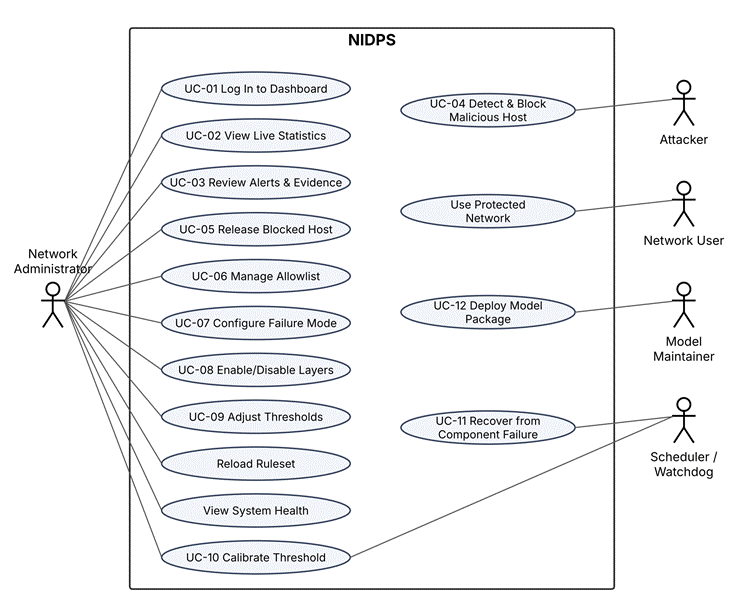
\includegraphics[width=0.99\textwidth,height=0.8\textheight,keepaspectratio]{Figures/usecase.png}
\caption{Use case diagram of the NIDPS.}
\label{fig:4.1}
\end{figure}

{\small
\begin{longtable}{|p{\dimexpr 0.060\linewidth-2\tabcolsep-1.3\arrayrulewidth\relax}|>{\raggedright\arraybackslash}p{\dimexpr 0.400\linewidth-2\tabcolsep-1.3\arrayrulewidth\relax}|p{\dimexpr 0.070\linewidth-2\tabcolsep-1.3\arrayrulewidth\relax}|>{\raggedright\arraybackslash}p{\dimexpr 0.470\linewidth-2\tabcolsep-1.3\arrayrulewidth\relax}|}
\caption{Use case UC-01: Log In to Dashboard.}\label{tab:4.3}\\
\hline
\endfirsthead
\hline
\endhead
\multicolumn{2}{|>{\raggedright\arraybackslash}p{\dimexpr 0.46\linewidth-2\tabcolsep\relax}|}{\textbf{Name}} & \multicolumn{2}{>{\raggedright\arraybackslash}p{\dimexpr 0.54\linewidth-2\tabcolsep-2\arrayrulewidth\relax}|}{\textbf{UC-01: Log In to Dashboard}} \\ \hline
\multicolumn{2}{|>{\raggedright\arraybackslash}p{\dimexpr 0.46\linewidth-2\tabcolsep\relax}|}{\textbf{Actors}} & \multicolumn{2}{>{\raggedright\arraybackslash}p{\dimexpr 0.54\linewidth-2\tabcolsep-2\arrayrulewidth\relax}|}{Network Administrator} \\ \hline
\multicolumn{2}{|>{\raggedright\arraybackslash}p{\dimexpr 0.46\linewidth-2\tabcolsep\relax}|}{\textbf{Summary}} & \multicolumn{2}{>{\raggedright\arraybackslash}p{\dimexpr 0.54\linewidth-2\tabcolsep-2\arrayrulewidth\relax}|}{The administrator enters a username and password on the login page. After successful verification, the system establishes a session and shows the overview page.} \\ \hline
\multicolumn{2}{|>{\raggedright\arraybackslash}p{\dimexpr 0.46\linewidth-2\tabcolsep\relax}|}{\textbf{Pre-Conditions}} & \multicolumn{2}{>{\raggedright\arraybackslash}p{\dimexpr 0.54\linewidth-2\tabcolsep-2\arrayrulewidth\relax}|}{The administrator's device is connected to the NIDPS network (LAN side).\newline An administrator account exists.\newline The administrator is not already logged in.} \\ \hline
\multicolumn{2}{|>{\raggedright\arraybackslash}p{\dimexpr 0.46\linewidth-2\tabcolsep\relax}|}{\textbf{Post-Conditions}} & \multicolumn{2}{>{\raggedright\arraybackslash}p{\dimexpr 0.54\linewidth-2\tabcolsep-2\arrayrulewidth\relax}|}{An authenticated session is established and the overview page is displayed.} \\ \hline
\multicolumn{2}{|>{\raggedright\arraybackslash}p{\dimexpr 0.46\linewidth-2\tabcolsep\relax}|}{\textbf{Special Requirements}} & \multicolumn{2}{>{\raggedright\arraybackslash}p{\dimexpr 0.54\linewidth-2\tabcolsep-2\arrayrulewidth\relax}|}{Passwords are stored as salted hashes. The account is locked for 5 minutes after 5 consecutive failed attempts (NFR-12).} \\ \hline
\multicolumn{4}{|c|}{\textbf{Basic Flow}} \\ \hline
\multicolumn{2}{|c|}{\textbf{Actor Action}} & \multicolumn{2}{c|}{\textbf{System Response}} \\ \hline
1 & The administrator opens the dashboard address in a browser. & 2 & The system displays the login page asking for username and password. \\ \hline
3 & The administrator enters a valid username and password and presses Log In. & 4 & The system verifies the credentials, creates a session, records the login in the audit log and displays the overview page. \\ \hline
\multicolumn{4}{|c|}{\textbf{Alternative Flow}} \\ \hline
3 & The administrator enters an invalid username or password. & 4-A & The system shows the message "Incorrect username or password" and increments the failed-attempt counter. \\ \hline
3 & The administrator enters wrong credentials for the fifth consecutive time. & 4-B & The system locks the account for 5 minutes and shows the time remaining. \\ \hline
\end{longtable}
}

{\small
\begin{longtable}{|p{\dimexpr 0.060\linewidth-2\tabcolsep-1.3\arrayrulewidth\relax}|>{\raggedright\arraybackslash}p{\dimexpr 0.400\linewidth-2\tabcolsep-1.3\arrayrulewidth\relax}|p{\dimexpr 0.070\linewidth-2\tabcolsep-1.3\arrayrulewidth\relax}|>{\raggedright\arraybackslash}p{\dimexpr 0.470\linewidth-2\tabcolsep-1.3\arrayrulewidth\relax}|}
\caption{Use case UC-02: View Live Network Statistics.}\label{tab:4.4}\\
\hline
\endfirsthead
\hline
\endhead
\multicolumn{2}{|>{\raggedright\arraybackslash}p{\dimexpr 0.46\linewidth-2\tabcolsep\relax}|}{\textbf{Name}} & \multicolumn{2}{>{\raggedright\arraybackslash}p{\dimexpr 0.54\linewidth-2\tabcolsep-2\arrayrulewidth\relax}|}{\textbf{UC-02: View Live Network Statistics}} \\ \hline
\multicolumn{2}{|>{\raggedright\arraybackslash}p{\dimexpr 0.46\linewidth-2\tabcolsep\relax}|}{\textbf{Actors}} & \multicolumn{2}{>{\raggedright\arraybackslash}p{\dimexpr 0.54\linewidth-2\tabcolsep-2\arrayrulewidth\relax}|}{Network Administrator} \\ \hline
\multicolumn{2}{|>{\raggedright\arraybackslash}p{\dimexpr 0.46\linewidth-2\tabcolsep\relax}|}{\textbf{Summary}} & \multicolumn{2}{>{\raggedright\arraybackslash}p{\dimexpr 0.54\linewidth-2\tabcolsep-2\arrayrulewidth\relax}|}{The administrator views real-time throughput, flows per second, alert and block counts per detection layer, attack category distribution and per-device traffic.} \\ \hline
\multicolumn{2}{|>{\raggedright\arraybackslash}p{\dimexpr 0.46\linewidth-2\tabcolsep\relax}|}{\textbf{Pre-Conditions}} & \multicolumn{2}{>{\raggedright\arraybackslash}p{\dimexpr 0.54\linewidth-2\tabcolsep-2\arrayrulewidth\relax}|}{The administrator is logged in (UC-01).} \\ \hline
\multicolumn{2}{|>{\raggedright\arraybackslash}p{\dimexpr 0.46\linewidth-2\tabcolsep\relax}|}{\textbf{Post-Conditions}} & \multicolumn{2}{>{\raggedright\arraybackslash}p{\dimexpr 0.54\linewidth-2\tabcolsep-2\arrayrulewidth\relax}|}{Live statistics are displayed and keep updating while the page is open.} \\ \hline
\multicolumn{2}{|>{\raggedright\arraybackslash}p{\dimexpr 0.46\linewidth-2\tabcolsep\relax}|}{\textbf{Special Requirements}} & \multicolumn{2}{>{\raggedright\arraybackslash}p{\dimexpr 0.54\linewidth-2\tabcolsep-2\arrayrulewidth\relax}|}{Statistics refresh at least every 2 seconds (FR-9.2).} \\ \hline
\multicolumn{4}{|c|}{\textbf{Basic Flow}} \\ \hline
\multicolumn{2}{|c|}{\textbf{Actor Action}} & \multicolumn{2}{c|}{\textbf{System Response}} \\ \hline
1 & The administrator opens the Overview page. & 2 & The system displays current throughput, flows per second, alerts and blocks per layer and the attack category chart for the last hour. \\ \hline
3 & The administrator selects a different time window (for example 24 hours). & 4 & The system reloads the charts and counters for the selected window. \\ \hline
5 & The administrator selects a client device from the device list. & 6 & The system shows that device's traffic summary and current risk score. \\ \hline
\multicolumn{4}{|c|}{\textbf{Alternative Flow}} \\ \hline
2 & No traffic has been observed in the selected window. & 2-A & The system shows empty charts with the message "No traffic in this period". \\ \hline
 & The live connection to the server is lost. &  & The system marks the data as stale and retries the connection automatically. \\ \hline
\end{longtable}
}

{\small
\begin{longtable}{|p{\dimexpr 0.060\linewidth-2\tabcolsep-1.3\arrayrulewidth\relax}|>{\raggedright\arraybackslash}p{\dimexpr 0.400\linewidth-2\tabcolsep-1.3\arrayrulewidth\relax}|p{\dimexpr 0.070\linewidth-2\tabcolsep-1.3\arrayrulewidth\relax}|>{\raggedright\arraybackslash}p{\dimexpr 0.470\linewidth-2\tabcolsep-1.3\arrayrulewidth\relax}|}
\caption{Use case UC-03: Review Alerts and Evidence.}\label{tab:4.5}\\
\hline
\endfirsthead
\hline
\endhead
\multicolumn{2}{|>{\raggedright\arraybackslash}p{\dimexpr 0.46\linewidth-2\tabcolsep\relax}|}{\textbf{Name}} & \multicolumn{2}{>{\raggedright\arraybackslash}p{\dimexpr 0.54\linewidth-2\tabcolsep-2\arrayrulewidth\relax}|}{\textbf{UC-03: Review Alerts and Evidence}} \\ \hline
\multicolumn{2}{|>{\raggedright\arraybackslash}p{\dimexpr 0.46\linewidth-2\tabcolsep\relax}|}{\textbf{Actors}} & \multicolumn{2}{>{\raggedright\arraybackslash}p{\dimexpr 0.54\linewidth-2\tabcolsep-2\arrayrulewidth\relax}|}{Network Administrator} \\ \hline
\multicolumn{2}{|>{\raggedright\arraybackslash}p{\dimexpr 0.46\linewidth-2\tabcolsep\relax}|}{\textbf{Summary}} & \multicolumn{2}{>{\raggedright\arraybackslash}p{\dimexpr 0.54\linewidth-2\tabcolsep-2\arrayrulewidth\relax}|}{The administrator browses the alert list, filters it and opens an alert to see which layer detected it, the evidence behind the verdict and the originating flow.} \\ \hline
\multicolumn{2}{|>{\raggedright\arraybackslash}p{\dimexpr 0.46\linewidth-2\tabcolsep\relax}|}{\textbf{Pre-Conditions}} & \multicolumn{2}{>{\raggedright\arraybackslash}p{\dimexpr 0.54\linewidth-2\tabcolsep-2\arrayrulewidth\relax}|}{The administrator is logged in (UC-01).} \\ \hline
\multicolumn{2}{|>{\raggedright\arraybackslash}p{\dimexpr 0.46\linewidth-2\tabcolsep\relax}|}{\textbf{Post-Conditions}} & \multicolumn{2}{>{\raggedright\arraybackslash}p{\dimexpr 0.54\linewidth-2\tabcolsep-2\arrayrulewidth\relax}|}{The selected alert and its evidence are displayed. The alert may be marked as reviewed.} \\ \hline
\multicolumn{2}{|>{\raggedright\arraybackslash}p{\dimexpr 0.46\linewidth-2\tabcolsep\relax}|}{\textbf{Special Requirements}} & \multicolumn{2}{>{\raggedright\arraybackslash}p{\dimexpr 0.54\linewidth-2\tabcolsep-2\arrayrulewidth\relax}|}{Each alert includes a plain-language description of the suspected attack (NFR-16).} \\ \hline
\multicolumn{4}{|c|}{\textbf{Basic Flow}} \\ \hline
\multicolumn{2}{|c|}{\textbf{Actor Action}} & \multicolumn{2}{c|}{\textbf{System Response}} \\ \hline
1 & The administrator opens the Alerts page. & 2 & The system displays the most recent alerts with time, source, destination, attack class, detecting layer, confidence and verdict. \\ \hline
3 & The administrator filters by severity, layer, host or time range. & 4 & The system displays only the matching alerts. \\ \hline
5 & The administrator selects an alert. & 6 & The system shows the evidence panel: Suricata signature, anomaly score and threshold, class probabilities, host risk history and the flow record. \\ \hline
7 & The administrator marks the alert as reviewed. & 8 & The system records the review in the audit log. \\ \hline
\multicolumn{4}{|c|}{\textbf{Alternative Flow}} \\ \hline
2 & No alerts match the filter. & 2-A & The system shows "No alerts match the selected filters". \\ \hline
3 & The flow record has been deleted by the retention policy. & 3-A & The system shows the stored evidence and notes that the flow details are no longer available. \\ \hline
\end{longtable}
}

{\small
\begin{longtable}{|p{\dimexpr 0.060\linewidth-2\tabcolsep-1.3\arrayrulewidth\relax}|>{\raggedright\arraybackslash}p{\dimexpr 0.400\linewidth-2\tabcolsep-1.3\arrayrulewidth\relax}|p{\dimexpr 0.070\linewidth-2\tabcolsep-1.3\arrayrulewidth\relax}|>{\raggedright\arraybackslash}p{\dimexpr 0.470\linewidth-2\tabcolsep-1.3\arrayrulewidth\relax}|}
\caption{Use case UC-04: Detect and Block Malicious Host.}\label{tab:4.6}\\
\hline
\endfirsthead
\hline
\endhead
\multicolumn{2}{|>{\raggedright\arraybackslash}p{\dimexpr 0.46\linewidth-2\tabcolsep\relax}|}{\textbf{Name}} & \multicolumn{2}{>{\raggedright\arraybackslash}p{\dimexpr 0.54\linewidth-2\tabcolsep-2\arrayrulewidth\relax}|}{\textbf{UC-04: Detect and Block Malicious Host}} \\ \hline
\multicolumn{2}{|>{\raggedright\arraybackslash}p{\dimexpr 0.46\linewidth-2\tabcolsep\relax}|}{\textbf{Actors}} & \multicolumn{2}{>{\raggedright\arraybackslash}p{\dimexpr 0.54\linewidth-2\tabcolsep-2\arrayrulewidth\relax}|}{Attacker (initiator), System} \\ \hline
\multicolumn{2}{|>{\raggedright\arraybackslash}p{\dimexpr 0.46\linewidth-2\tabcolsep\relax}|}{\textbf{Summary}} & \multicolumn{2}{>{\raggedright\arraybackslash}p{\dimexpr 0.54\linewidth-2\tabcolsep-2\arrayrulewidth\relax}|}{Traffic from an attacker is detected by one or more layers. The decision engine issues a BLOCK verdict, and the enforcer adds the attacker's address to the block set for a limited time and notifies the dashboard.} \\ \hline
\multicolumn{2}{|>{\raggedright\arraybackslash}p{\dimexpr 0.46\linewidth-2\tabcolsep\relax}|}{\textbf{Pre-Conditions}} & \multicolumn{2}{>{\raggedright\arraybackslash}p{\dimexpr 0.54\linewidth-2\tabcolsep-2\arrayrulewidth\relax}|}{The NIDPS is running with at least one detection layer enabled.\newline The attacker's traffic passes through the NIDPS.} \\ \hline
\multicolumn{2}{|>{\raggedright\arraybackslash}p{\dimexpr 0.46\linewidth-2\tabcolsep\relax}|}{\textbf{Post-Conditions}} & \multicolumn{2}{>{\raggedright\arraybackslash}p{\dimexpr 0.54\linewidth-2\tabcolsep-2\arrayrulewidth\relax}|}{The attacker's address is in the block set with an expiry time.\newline An audit record and a dashboard event exist for the block.} \\ \hline
\multicolumn{2}{|>{\raggedright\arraybackslash}p{\dimexpr 0.46\linewidth-2\tabcolsep\relax}|}{\textbf{Special Requirements}} & \multicolumn{2}{>{\raggedright\arraybackslash}p{\dimexpr 0.54\linewidth-2\tabcolsep-2\arrayrulewidth\relax}|}{Blocking must take effect within 1 second of the verdict (NFR-4). Allowlisted addresses are never blocked (FR-7.3).} \\ \hline
\multicolumn{4}{|c|}{\textbf{Basic Flow}} \\ \hline
\multicolumn{2}{|c|}{\textbf{Actor Action}} & \multicolumn{2}{c|}{\textbf{System Response}} \\ \hline
1 & The attacker sends malicious traffic (for example an SSH brute-force attempt or a beaconing connection). & 2 & Suricata inspects the packets inline; the flow extractor builds flow records with features and TLS fingerprints. \\ \hline
 & --- & 3 & Layer 1 raises an alert and/or Layers 2 and 3 score the flow; the evidence is published on the event bus. \\ \hline
 & --- & 4 & The decision engine applies the verdict algorithm and returns BLOCK with the responsible layer(s). \\ \hline
 & --- & 5 & The enforcer checks the allowlist and rate limit, computes the block duration, adds the address to the ipset and writes an audit record. \\ \hline
6 & The attacker continues sending traffic. & 7 & Packets from the attacker are dropped in the kernel before reaching Suricata. The dashboard shows the new block. \\ \hline
\multicolumn{4}{|c|}{\textbf{Alternative Flow}} \\ \hline
3 & Evidence is weak (for example an anomaly score just above $\tau$ only). & 3-A & The verdict is ALERT; evidence is added to the host's risk score, and the host is blocked only if its score reaches $\Theta$. \\ \hline
4 & The attacker's address is on the allowlist. & 4-A & The block is suppressed and logged as "block suppressed"; an alert is still shown. \\ \hline
4 & The block rate limit R\_max has been reached. & 4-B & The verdict is downgraded to ALERT and a "block rate limit" warning is shown on the dashboard. \\ \hline
4 & The attacker was blocked before in the last 24 hours. & 4-C & The block duration is doubled for each earlier offence, up to the maximum. \\ \hline
\end{longtable}
}

{\small
\begin{longtable}{|p{\dimexpr 0.060\linewidth-2\tabcolsep-1.3\arrayrulewidth\relax}|>{\raggedright\arraybackslash}p{\dimexpr 0.400\linewidth-2\tabcolsep-1.3\arrayrulewidth\relax}|p{\dimexpr 0.070\linewidth-2\tabcolsep-1.3\arrayrulewidth\relax}|>{\raggedright\arraybackslash}p{\dimexpr 0.470\linewidth-2\tabcolsep-1.3\arrayrulewidth\relax}|}
\caption{Use case UC-05: Release Blocked Host.}\label{tab:4.7}\\
\hline
\endfirsthead
\hline
\endhead
\multicolumn{2}{|>{\raggedright\arraybackslash}p{\dimexpr 0.46\linewidth-2\tabcolsep\relax}|}{\textbf{Name}} & \multicolumn{2}{>{\raggedright\arraybackslash}p{\dimexpr 0.54\linewidth-2\tabcolsep-2\arrayrulewidth\relax}|}{\textbf{UC-05: Release Blocked Host}} \\ \hline
\multicolumn{2}{|>{\raggedright\arraybackslash}p{\dimexpr 0.46\linewidth-2\tabcolsep\relax}|}{\textbf{Actors}} & \multicolumn{2}{>{\raggedright\arraybackslash}p{\dimexpr 0.54\linewidth-2\tabcolsep-2\arrayrulewidth\relax}|}{Network Administrator} \\ \hline
\multicolumn{2}{|>{\raggedright\arraybackslash}p{\dimexpr 0.46\linewidth-2\tabcolsep\relax}|}{\textbf{Summary}} & \multicolumn{2}{>{\raggedright\arraybackslash}p{\dimexpr 0.54\linewidth-2\tabcolsep-2\arrayrulewidth\relax}|}{The administrator reviews the list of blocked hosts and manually releases a host that was blocked by mistake.} \\ \hline
\multicolumn{2}{|>{\raggedright\arraybackslash}p{\dimexpr 0.46\linewidth-2\tabcolsep\relax}|}{\textbf{Pre-Conditions}} & \multicolumn{2}{>{\raggedright\arraybackslash}p{\dimexpr 0.54\linewidth-2\tabcolsep-2\arrayrulewidth\relax}|}{The administrator is logged in (UC-01).\newline At least one host is currently blocked.} \\ \hline
\multicolumn{2}{|>{\raggedright\arraybackslash}p{\dimexpr 0.46\linewidth-2\tabcolsep\relax}|}{\textbf{Post-Conditions}} & \multicolumn{2}{>{\raggedright\arraybackslash}p{\dimexpr 0.54\linewidth-2\tabcolsep-2\arrayrulewidth\relax}|}{The host's address is removed from the block set and the release is recorded in the audit log.} \\ \hline
\multicolumn{2}{|>{\raggedright\arraybackslash}p{\dimexpr 0.46\linewidth-2\tabcolsep\relax}|}{\textbf{Special Requirements}} & \multicolumn{2}{>{\raggedright\arraybackslash}p{\dimexpr 0.54\linewidth-2\tabcolsep-2\arrayrulewidth\relax}|}{The released host may optionally be added to the allowlist (UC-06).} \\ \hline
\multicolumn{4}{|c|}{\textbf{Basic Flow}} \\ \hline
\multicolumn{2}{|c|}{\textbf{Actor Action}} & \multicolumn{2}{c|}{\textbf{System Response}} \\ \hline
1 & The administrator opens the Blocked Hosts page. & 2 & The system lists blocked hosts with address, device name, attack class, detecting layer, block start and remaining time. \\ \hline
3 & The administrator selects a host and presses Release. & 4 & The system asks for confirmation and offers to add the host to the allowlist. \\ \hline
5 & The administrator confirms. & 6 & The system removes the address from the ipset, marks the block as released, writes an audit record and refreshes the list. \\ \hline
\multicolumn{4}{|c|}{\textbf{Alternative Flow}} \\ \hline
3 & The block expired while the dialog was open. & 3-A & The system informs the administrator that the block has already expired. \\ \hline
3 & The administrator cancels. & 3-B & No change is made. \\ \hline
\end{longtable}
}

{\small
\begin{longtable}{|p{\dimexpr 0.060\linewidth-2\tabcolsep-1.3\arrayrulewidth\relax}|>{\raggedright\arraybackslash}p{\dimexpr 0.400\linewidth-2\tabcolsep-1.3\arrayrulewidth\relax}|p{\dimexpr 0.070\linewidth-2\tabcolsep-1.3\arrayrulewidth\relax}|>{\raggedright\arraybackslash}p{\dimexpr 0.470\linewidth-2\tabcolsep-1.3\arrayrulewidth\relax}|}
\caption{Use case UC-06: Manage Allowlist.}\label{tab:4.8}\\
\hline
\endfirsthead
\hline
\endhead
\multicolumn{2}{|>{\raggedright\arraybackslash}p{\dimexpr 0.46\linewidth-2\tabcolsep\relax}|}{\textbf{Name}} & \multicolumn{2}{>{\raggedright\arraybackslash}p{\dimexpr 0.54\linewidth-2\tabcolsep-2\arrayrulewidth\relax}|}{\textbf{UC-06: Manage Allowlist}} \\ \hline
\multicolumn{2}{|>{\raggedright\arraybackslash}p{\dimexpr 0.46\linewidth-2\tabcolsep\relax}|}{\textbf{Actors}} & \multicolumn{2}{>{\raggedright\arraybackslash}p{\dimexpr 0.54\linewidth-2\tabcolsep-2\arrayrulewidth\relax}|}{Network Administrator} \\ \hline
\multicolumn{2}{|>{\raggedright\arraybackslash}p{\dimexpr 0.46\linewidth-2\tabcolsep\relax}|}{\textbf{Summary}} & \multicolumn{2}{>{\raggedright\arraybackslash}p{\dimexpr 0.54\linewidth-2\tabcolsep-2\arrayrulewidth\relax}|}{The administrator adds or removes IP or MAC addresses that must never be blocked, such as the gateway or the administrator's own laptop.} \\ \hline
\multicolumn{2}{|>{\raggedright\arraybackslash}p{\dimexpr 0.46\linewidth-2\tabcolsep\relax}|}{\textbf{Pre-Conditions}} & \multicolumn{2}{>{\raggedright\arraybackslash}p{\dimexpr 0.54\linewidth-2\tabcolsep-2\arrayrulewidth\relax}|}{The administrator is logged in (UC-01).} \\ \hline
\multicolumn{2}{|>{\raggedright\arraybackslash}p{\dimexpr 0.46\linewidth-2\tabcolsep\relax}|}{\textbf{Post-Conditions}} & \multicolumn{2}{>{\raggedright\arraybackslash}p{\dimexpr 0.54\linewidth-2\tabcolsep-2\arrayrulewidth\relax}|}{The allowlist is updated and immediately used by the enforcer.} \\ \hline
\multicolumn{2}{|>{\raggedright\arraybackslash}p{\dimexpr 0.46\linewidth-2\tabcolsep\relax}|}{\textbf{Special Requirements}} & \multicolumn{2}{>{\raggedright\arraybackslash}p{\dimexpr 0.54\linewidth-2\tabcolsep-2\arrayrulewidth\relax}|}{The NIDPS host, gateway and DNS resolver are permanent entries and cannot be removed.} \\ \hline
\multicolumn{4}{|c|}{\textbf{Basic Flow}} \\ \hline
\multicolumn{2}{|c|}{\textbf{Actor Action}} & \multicolumn{2}{c|}{\textbf{System Response}} \\ \hline
1 & The administrator opens the Allowlist section and presses Add. & 2 & The system shows a form for address and description. \\ \hline
3 & The administrator enters an address and description and saves. & 4 & The system validates the address, stores the entry, publishes the change on the bus and records it in the audit log. \\ \hline
\multicolumn{4}{|c|}{\textbf{Alternative Flow}} \\ \hline
2 & The address is invalid or already listed. & 2-A & The system shows a validation error and does not save. \\ \hline
2 & The address is currently blocked. & 2-B & The system asks whether to release the block as well (UC-05). \\ \hline
\end{longtable}
}

{\small
\begin{longtable}{|p{\dimexpr 0.060\linewidth-2\tabcolsep-1.3\arrayrulewidth\relax}|>{\raggedright\arraybackslash}p{\dimexpr 0.400\linewidth-2\tabcolsep-1.3\arrayrulewidth\relax}|p{\dimexpr 0.070\linewidth-2\tabcolsep-1.3\arrayrulewidth\relax}|>{\raggedright\arraybackslash}p{\dimexpr 0.470\linewidth-2\tabcolsep-1.3\arrayrulewidth\relax}|}
\caption{Use case UC-07: Configure Failure Mode.}\label{tab:4.9}\\
\hline
\endfirsthead
\hline
\endhead
\multicolumn{2}{|>{\raggedright\arraybackslash}p{\dimexpr 0.46\linewidth-2\tabcolsep\relax}|}{\textbf{Name}} & \multicolumn{2}{>{\raggedright\arraybackslash}p{\dimexpr 0.54\linewidth-2\tabcolsep-2\arrayrulewidth\relax}|}{\textbf{UC-07: Configure Failure Mode}} \\ \hline
\multicolumn{2}{|>{\raggedright\arraybackslash}p{\dimexpr 0.46\linewidth-2\tabcolsep\relax}|}{\textbf{Actors}} & \multicolumn{2}{>{\raggedright\arraybackslash}p{\dimexpr 0.54\linewidth-2\tabcolsep-2\arrayrulewidth\relax}|}{Network Administrator} \\ \hline
\multicolumn{2}{|>{\raggedright\arraybackslash}p{\dimexpr 0.46\linewidth-2\tabcolsep\relax}|}{\textbf{Summary}} & \multicolumn{2}{>{\raggedright\arraybackslash}p{\dimexpr 0.54\linewidth-2\tabcolsep-2\arrayrulewidth\relax}|}{The administrator chooses how the network behaves when a detection component fails: fail-open (keep internet access), fail-closed (stop forwarding until detection is restored) or degraded operation under load.} \\ \hline
\multicolumn{2}{|>{\raggedright\arraybackslash}p{\dimexpr 0.46\linewidth-2\tabcolsep\relax}|}{\textbf{Pre-Conditions}} & \multicolumn{2}{>{\raggedright\arraybackslash}p{\dimexpr 0.54\linewidth-2\tabcolsep-2\arrayrulewidth\relax}|}{The administrator is logged in (UC-01).} \\ \hline
\multicolumn{2}{|>{\raggedright\arraybackslash}p{\dimexpr 0.46\linewidth-2\tabcolsep\relax}|}{\textbf{Post-Conditions}} & \multicolumn{2}{>{\raggedright\arraybackslash}p{\dimexpr 0.54\linewidth-2\tabcolsep-2\arrayrulewidth\relax}|}{The new failure mode is saved and applied to the kernel queue configuration.} \\ \hline
\multicolumn{2}{|>{\raggedright\arraybackslash}p{\dimexpr 0.46\linewidth-2\tabcolsep\relax}|}{\textbf{Special Requirements}} & \multicolumn{2}{>{\raggedright\arraybackslash}p{\dimexpr 0.54\linewidth-2\tabcolsep-2\arrayrulewidth\relax}|}{Changing between fail-open and fail-closed briefly reloads the inspection queue rule; forwarding is not interrupted.} \\ \hline
\multicolumn{4}{|c|}{\textbf{Basic Flow}} \\ \hline
\multicolumn{2}{|c|}{\textbf{Actor Action}} & \multicolumn{2}{c|}{\textbf{System Response}} \\ \hline
1 & The administrator opens Settings and selects the Failure Mode tab. & 2 & The system shows the current mode with a description of its trade-off. \\ \hline
3 & The administrator selects a new mode and presses Save. & 4 & The system asks for confirmation, explaining the effect of the chosen mode. \\ \hline
5 & The administrator confirms. & 6 & The system updates the queue-bypass setting, saves the configuration, logs the change and shows a success message. \\ \hline
\multicolumn{4}{|c|}{\textbf{Alternative Flow}} \\ \hline
3 & The system cannot apply the new rule. & 3-A & The previous mode remains active and an error message is shown. \\ \hline
\end{longtable}
}

{\small
\begin{longtable}{|p{\dimexpr 0.060\linewidth-2\tabcolsep-1.3\arrayrulewidth\relax}|>{\raggedright\arraybackslash}p{\dimexpr 0.400\linewidth-2\tabcolsep-1.3\arrayrulewidth\relax}|p{\dimexpr 0.070\linewidth-2\tabcolsep-1.3\arrayrulewidth\relax}|>{\raggedright\arraybackslash}p{\dimexpr 0.470\linewidth-2\tabcolsep-1.3\arrayrulewidth\relax}|}
\caption{Use case UC-08: Enable or Disable Detection Layers.}\label{tab:4.10}\\
\hline
\endfirsthead
\hline
\endhead
\multicolumn{2}{|>{\raggedright\arraybackslash}p{\dimexpr 0.46\linewidth-2\tabcolsep\relax}|}{\textbf{Name}} & \multicolumn{2}{>{\raggedright\arraybackslash}p{\dimexpr 0.54\linewidth-2\tabcolsep-2\arrayrulewidth\relax}|}{\textbf{UC-08: Enable or Disable Detection Layers}} \\ \hline
\multicolumn{2}{|>{\raggedright\arraybackslash}p{\dimexpr 0.46\linewidth-2\tabcolsep\relax}|}{\textbf{Actors}} & \multicolumn{2}{>{\raggedright\arraybackslash}p{\dimexpr 0.54\linewidth-2\tabcolsep-2\arrayrulewidth\relax}|}{Network Administrator} \\ \hline
\multicolumn{2}{|>{\raggedright\arraybackslash}p{\dimexpr 0.46\linewidth-2\tabcolsep\relax}|}{\textbf{Summary}} & \multicolumn{2}{>{\raggedright\arraybackslash}p{\dimexpr 0.54\linewidth-2\tabcolsep-2\arrayrulewidth\relax}|}{The administrator turns individual detection layers (Suricata, Isolation Forest, classifier) on or off. This is also used to run the layer ablation experiments.} \\ \hline
\multicolumn{2}{|>{\raggedright\arraybackslash}p{\dimexpr 0.46\linewidth-2\tabcolsep\relax}|}{\textbf{Pre-Conditions}} & \multicolumn{2}{>{\raggedright\arraybackslash}p{\dimexpr 0.54\linewidth-2\tabcolsep-2\arrayrulewidth\relax}|}{The administrator is logged in (UC-01).} \\ \hline
\multicolumn{2}{|>{\raggedright\arraybackslash}p{\dimexpr 0.46\linewidth-2\tabcolsep\relax}|}{\textbf{Post-Conditions}} & \multicolumn{2}{>{\raggedright\arraybackslash}p{\dimexpr 0.54\linewidth-2\tabcolsep-2\arrayrulewidth\relax}|}{The selected layers are active or inactive and the dashboard shows their status.} \\ \hline
\multicolumn{2}{|>{\raggedright\arraybackslash}p{\dimexpr 0.46\linewidth-2\tabcolsep\relax}|}{\textbf{Special Requirements}} & \multicolumn{2}{>{\raggedright\arraybackslash}p{\dimexpr 0.54\linewidth-2\tabcolsep-2\arrayrulewidth\relax}|}{At least one layer must remain enabled unless the administrator explicitly confirms monitoring-only operation.} \\ \hline
\multicolumn{4}{|c|}{\textbf{Basic Flow}} \\ \hline
\multicolumn{2}{|c|}{\textbf{Actor Action}} & \multicolumn{2}{c|}{\textbf{System Response}} \\ \hline
1 & The administrator opens Settings and selects the Detection Layers tab. & 2 & The system shows each layer with its status and a toggle. \\ \hline
3 & The administrator switches a layer off and saves. & 4 & The system publishes the change; the decision engine stops using that layer's evidence and the dashboard marks it as disabled. \\ \hline
5 & The administrator switches the layer back on. & 6 & The system resumes using the layer's evidence. \\ \hline
\multicolumn{4}{|c|}{\textbf{Alternative Flow}} \\ \hline
2 & The administrator tries to disable all layers. & 2-A & The system warns that the network will be unprotected and requires explicit confirmation. \\ \hline
\end{longtable}
}

{\small
\begin{longtable}{|p{\dimexpr 0.060\linewidth-2\tabcolsep-1.3\arrayrulewidth\relax}|>{\raggedright\arraybackslash}p{\dimexpr 0.400\linewidth-2\tabcolsep-1.3\arrayrulewidth\relax}|p{\dimexpr 0.070\linewidth-2\tabcolsep-1.3\arrayrulewidth\relax}|>{\raggedright\arraybackslash}p{\dimexpr 0.470\linewidth-2\tabcolsep-1.3\arrayrulewidth\relax}|}
\caption{Use case UC-09: Adjust Detection Thresholds.}\label{tab:4.11}\\
\hline
\endfirsthead
\hline
\endhead
\multicolumn{2}{|>{\raggedright\arraybackslash}p{\dimexpr 0.46\linewidth-2\tabcolsep\relax}|}{\textbf{Name}} & \multicolumn{2}{>{\raggedright\arraybackslash}p{\dimexpr 0.54\linewidth-2\tabcolsep-2\arrayrulewidth\relax}|}{\textbf{UC-09: Adjust Detection Thresholds}} \\ \hline
\multicolumn{2}{|>{\raggedright\arraybackslash}p{\dimexpr 0.46\linewidth-2\tabcolsep\relax}|}{\textbf{Actors}} & \multicolumn{2}{>{\raggedright\arraybackslash}p{\dimexpr 0.54\linewidth-2\tabcolsep-2\arrayrulewidth\relax}|}{Network Administrator} \\ \hline
\multicolumn{2}{|>{\raggedright\arraybackslash}p{\dimexpr 0.46\linewidth-2\tabcolsep\relax}|}{\textbf{Summary}} & \multicolumn{2}{>{\raggedright\arraybackslash}p{\dimexpr 0.54\linewidth-2\tabcolsep-2\arrayrulewidth\relax}|}{The administrator changes detection sensitivity, such as the calibration percentile, classifier confidence thresholds, host block threshold and block durations.} \\ \hline
\multicolumn{2}{|>{\raggedright\arraybackslash}p{\dimexpr 0.46\linewidth-2\tabcolsep\relax}|}{\textbf{Pre-Conditions}} & \multicolumn{2}{>{\raggedright\arraybackslash}p{\dimexpr 0.54\linewidth-2\tabcolsep-2\arrayrulewidth\relax}|}{The administrator is logged in (UC-01).} \\ \hline
\multicolumn{2}{|>{\raggedright\arraybackslash}p{\dimexpr 0.46\linewidth-2\tabcolsep\relax}|}{\textbf{Post-Conditions}} & \multicolumn{2}{>{\raggedright\arraybackslash}p{\dimexpr 0.54\linewidth-2\tabcolsep-2\arrayrulewidth\relax}|}{The new thresholds are validated, saved and used by running services.} \\ \hline
\multicolumn{2}{|>{\raggedright\arraybackslash}p{\dimexpr 0.46\linewidth-2\tabcolsep\relax}|}{\textbf{Special Requirements}} & \multicolumn{2}{>{\raggedright\arraybackslash}p{\dimexpr 0.54\linewidth-2\tabcolsep-2\arrayrulewidth\relax}|}{Each value has a validated range and a documented default, which can be restored with one action.} \\ \hline
\multicolumn{4}{|c|}{\textbf{Basic Flow}} \\ \hline
\multicolumn{2}{|c|}{\textbf{Actor Action}} & \multicolumn{2}{c|}{\textbf{System Response}} \\ \hline
1 & The administrator opens Settings and selects the Thresholds tab. & 2 & The system shows current values, defaults and allowed ranges. \\ \hline
3 & The administrator changes a value and presses Save. & 4 & The system validates the value, saves it, publishes the change and logs old and new values. \\ \hline
\multicolumn{4}{|c|}{\textbf{Alternative Flow}} \\ \hline
2 & The value is outside the allowed range. & 2-A & The system rejects the value and shows the allowed range. \\ \hline
2 & The administrator presses Restore Defaults. & 2-B & The system restores all default values after confirmation. \\ \hline
\end{longtable}
}

{\small
\begin{longtable}{|p{\dimexpr 0.060\linewidth-2\tabcolsep-1.3\arrayrulewidth\relax}|>{\raggedright\arraybackslash}p{\dimexpr 0.400\linewidth-2\tabcolsep-1.3\arrayrulewidth\relax}|p{\dimexpr 0.070\linewidth-2\tabcolsep-1.3\arrayrulewidth\relax}|>{\raggedright\arraybackslash}p{\dimexpr 0.470\linewidth-2\tabcolsep-1.3\arrayrulewidth\relax}|}
\caption{Use case UC-10: Calibrate Anomaly Threshold.}\label{tab:4.12}\\
\hline
\endfirsthead
\hline
\endhead
\multicolumn{2}{|>{\raggedright\arraybackslash}p{\dimexpr 0.46\linewidth-2\tabcolsep\relax}|}{\textbf{Name}} & \multicolumn{2}{>{\raggedright\arraybackslash}p{\dimexpr 0.54\linewidth-2\tabcolsep-2\arrayrulewidth\relax}|}{\textbf{UC-10: Calibrate Anomaly Threshold}} \\ \hline
\multicolumn{2}{|>{\raggedright\arraybackslash}p{\dimexpr 0.46\linewidth-2\tabcolsep\relax}|}{\textbf{Actors}} & \multicolumn{2}{>{\raggedright\arraybackslash}p{\dimexpr 0.54\linewidth-2\tabcolsep-2\arrayrulewidth\relax}|}{System Scheduler, Network Administrator} \\ \hline
\multicolumn{2}{|>{\raggedright\arraybackslash}p{\dimexpr 0.46\linewidth-2\tabcolsep\relax}|}{\textbf{Summary}} & \multicolumn{2}{>{\raggedright\arraybackslash}p{\dimexpr 0.54\linewidth-2\tabcolsep-2\arrayrulewidth\relax}|}{The anomaly threshold $\tau$ is recalculated from the scores of clean local traffic so that it fits the deployment network. It runs weekly or on demand.} \\ \hline
\multicolumn{2}{|>{\raggedright\arraybackslash}p{\dimexpr 0.46\linewidth-2\tabcolsep\relax}|}{\textbf{Pre-Conditions}} & \multicolumn{2}{>{\raggedright\arraybackslash}p{\dimexpr 0.54\linewidth-2\tabcolsep-2\arrayrulewidth\relax}|}{The Isolation Forest model is loaded.\newline Flow records from the calibration window are available.} \\ \hline
\multicolumn{2}{|>{\raggedright\arraybackslash}p{\dimexpr 0.46\linewidth-2\tabcolsep\relax}|}{\textbf{Post-Conditions}} & \multicolumn{2}{>{\raggedright\arraybackslash}p{\dimexpr 0.54\linewidth-2\tabcolsep-2\arrayrulewidth\relax}|}{A new calibration state ($\tau$, timestamp, sample count) is stored and used by Layer 2.} \\ \hline
\multicolumn{2}{|>{\raggedright\arraybackslash}p{\dimexpr 0.46\linewidth-2\tabcolsep\relax}|}{\textbf{Special Requirements}} & \multicolumn{2}{>{\raggedright\arraybackslash}p{\dimexpr 0.54\linewidth-2\tabcolsep-2\arrayrulewidth\relax}|}{Flows linked to Suricata alerts or blocked hosts are excluded, and $\tau$ cannot move more than $\delta$ from the global threshold (Algorithm~\ref{alg:calibration}).} \\ \hline
\multicolumn{4}{|c|}{\textbf{Basic Flow}} \\ \hline
\multicolumn{2}{|c|}{\textbf{Actor Action}} & \multicolumn{2}{c|}{\textbf{System Response}} \\ \hline
1 & The scheduler triggers calibration (or the administrator presses Recalibrate Now). & 2 & The system collects anomaly scores of the clean flows from the calibration window. \\ \hline
 & --- & 3 & The system computes the p-th percentile, clips it to the allowed range, stores the new $\tau$ and publishes it on the bus. \\ \hline
 & --- & 4 & The dashboard shows the new $\tau$, its date and the number of flows used. \\ \hline
\multicolumn{4}{|c|}{\textbf{Alternative Flow}} \\ \hline
2 & Fewer than N\_min clean flows are available. & 2-A & The system keeps the global threshold and reports that more traffic is needed. \\ \hline
\end{longtable}
}

{\small
\begin{longtable}{|p{\dimexpr 0.060\linewidth-2\tabcolsep-1.3\arrayrulewidth\relax}|>{\raggedright\arraybackslash}p{\dimexpr 0.400\linewidth-2\tabcolsep-1.3\arrayrulewidth\relax}|p{\dimexpr 0.070\linewidth-2\tabcolsep-1.3\arrayrulewidth\relax}|>{\raggedright\arraybackslash}p{\dimexpr 0.470\linewidth-2\tabcolsep-1.3\arrayrulewidth\relax}|}
\caption{Use case UC-11: Recover from Component Failure.}\label{tab:4.13}\\
\hline
\endfirsthead
\hline
\endhead
\multicolumn{2}{|>{\raggedright\arraybackslash}p{\dimexpr 0.46\linewidth-2\tabcolsep\relax}|}{\textbf{Name}} & \multicolumn{2}{>{\raggedright\arraybackslash}p{\dimexpr 0.54\linewidth-2\tabcolsep-2\arrayrulewidth\relax}|}{\textbf{UC-11: Recover from Component Failure}} \\ \hline
\multicolumn{2}{|>{\raggedright\arraybackslash}p{\dimexpr 0.46\linewidth-2\tabcolsep\relax}|}{\textbf{Actors}} & \multicolumn{2}{>{\raggedright\arraybackslash}p{\dimexpr 0.54\linewidth-2\tabcolsep-2\arrayrulewidth\relax}|}{Watchdog} \\ \hline
\multicolumn{2}{|>{\raggedright\arraybackslash}p{\dimexpr 0.46\linewidth-2\tabcolsep\relax}|}{\textbf{Summary}} & \multicolumn{2}{>{\raggedright\arraybackslash}p{\dimexpr 0.54\linewidth-2\tabcolsep-2\arrayrulewidth\relax}|}{When a component crashes, freezes or is overloaded, the watchdog detects it, applies the configured failure mode, restarts the component and records the recovery.} \\ \hline
\multicolumn{2}{|>{\raggedright\arraybackslash}p{\dimexpr 0.46\linewidth-2\tabcolsep\relax}|}{\textbf{Pre-Conditions}} & \multicolumn{2}{>{\raggedright\arraybackslash}p{\dimexpr 0.54\linewidth-2\tabcolsep-2\arrayrulewidth\relax}|}{The watchdog is running and receiving heartbeats.} \\ \hline
\multicolumn{2}{|>{\raggedright\arraybackslash}p{\dimexpr 0.46\linewidth-2\tabcolsep\relax}|}{\textbf{Post-Conditions}} & \multicolumn{2}{>{\raggedright\arraybackslash}p{\dimexpr 0.54\linewidth-2\tabcolsep-2\arrayrulewidth\relax}|}{The component is running again, or the system remains in the configured failure mode and the administrator is notified.} \\ \hline
\multicolumn{2}{|>{\raggedright\arraybackslash}p{\dimexpr 0.46\linewidth-2\tabcolsep\relax}|}{\textbf{Special Requirements}} & \multicolumn{2}{>{\raggedright\arraybackslash}p{\dimexpr 0.54\linewidth-2\tabcolsep-2\arrayrulewidth\relax}|}{Detection within 3 seconds and restart within 30 seconds (NFR-8). Fail-open is enforced by the kernel even if the watchdog itself fails.} \\ \hline
\multicolumn{4}{|c|}{\textbf{Basic Flow}} \\ \hline
\multicolumn{2}{|c|}{\textbf{Actor Action}} & \multicolumn{2}{c|}{\textbf{System Response}} \\ \hline
 & --- & 1 & A component misses three consecutive heartbeats or its process exits. \\ \hline
 & --- & 2 & The watchdog declares it failed, applies the failure mode and logs the failure event. \\ \hline
 & --- & 3 & systemd restarts the component; the watchdog waits for healthy heartbeats. \\ \hline
 & --- & 4 & The watchdog marks the component as running, restores normal mode and records the recovery time and packets dropped or bypassed. \\ \hline
5 & The administrator views System Health. & 6 & The system shows the failure event and recovery details. \\ \hline
\multicolumn{4}{|c|}{\textbf{Alternative Flow}} \\ \hline
3 & The component fails to restart after the maximum number of attempts. & 3-A & The system stays in the failure mode and shows a critical warning on the dashboard. \\ \hline
1 & Load exceeds the high watermark without a crash. & 2-A & The watchdog enters degraded mode and returns to normal when load falls below the low watermark. \\ \hline
\end{longtable}
}

{\small
\begin{longtable}{|p{\dimexpr 0.060\linewidth-2\tabcolsep-1.3\arrayrulewidth\relax}|>{\raggedright\arraybackslash}p{\dimexpr 0.400\linewidth-2\tabcolsep-1.3\arrayrulewidth\relax}|p{\dimexpr 0.070\linewidth-2\tabcolsep-1.3\arrayrulewidth\relax}|>{\raggedright\arraybackslash}p{\dimexpr 0.470\linewidth-2\tabcolsep-1.3\arrayrulewidth\relax}|}
\caption{Use case UC-12: Deploy Model Package.}\label{tab:4.14}\\
\hline
\endfirsthead
\hline
\endhead
\multicolumn{2}{|>{\raggedright\arraybackslash}p{\dimexpr 0.46\linewidth-2\tabcolsep\relax}|}{\textbf{Name}} & \multicolumn{2}{>{\raggedright\arraybackslash}p{\dimexpr 0.54\linewidth-2\tabcolsep-2\arrayrulewidth\relax}|}{\textbf{UC-12: Deploy Model Package}} \\ \hline
\multicolumn{2}{|>{\raggedright\arraybackslash}p{\dimexpr 0.46\linewidth-2\tabcolsep\relax}|}{\textbf{Actors}} & \multicolumn{2}{>{\raggedright\arraybackslash}p{\dimexpr 0.54\linewidth-2\tabcolsep-2\arrayrulewidth\relax}|}{Model Maintainer} \\ \hline
\multicolumn{2}{|>{\raggedright\arraybackslash}p{\dimexpr 0.46\linewidth-2\tabcolsep\relax}|}{\textbf{Summary}} & \multicolumn{2}{>{\raggedright\arraybackslash}p{\dimexpr 0.54\linewidth-2\tabcolsep-2\arrayrulewidth\relax}|}{The maintainer trains and validates a new model offline and deploys it to the device as a versioned package. The device checks compatibility before using it.} \\ \hline
\multicolumn{2}{|>{\raggedright\arraybackslash}p{\dimexpr 0.46\linewidth-2\tabcolsep\relax}|}{\textbf{Pre-Conditions}} & \multicolumn{2}{>{\raggedright\arraybackslash}p{\dimexpr 0.54\linewidth-2\tabcolsep-2\arrayrulewidth\relax}|}{A model package has been produced by the offline training pipeline (FR-12.3).\newline The maintainer has deployment access to the device.} \\ \hline
\multicolumn{2}{|>{\raggedright\arraybackslash}p{\dimexpr 0.46\linewidth-2\tabcolsep\relax}|}{\textbf{Post-Conditions}} & \multicolumn{2}{>{\raggedright\arraybackslash}p{\dimexpr 0.54\linewidth-2\tabcolsep-2\arrayrulewidth\relax}|}{The new model is active and the previous package is kept for rollback.} \\ \hline
\multicolumn{2}{|>{\raggedright\arraybackslash}p{\dimexpr 0.46\linewidth-2\tabcolsep\relax}|}{\textbf{Special Requirements}} & \multicolumn{2}{>{\raggedright\arraybackslash}p{\dimexpr 0.54\linewidth-2\tabcolsep-2\arrayrulewidth\relax}|}{XGBoost models are stored in native JSON format; packages are loaded only from the protected registry directory.} \\ \hline
\multicolumn{4}{|c|}{\textbf{Basic Flow}} \\ \hline
\multicolumn{2}{|c|}{\textbf{Actor Action}} & \multicolumn{2}{c|}{\textbf{System Response}} \\ \hline
1 & The maintainer copies the package to the model registry and runs the deploy command. & 2 & The system checks the feature list and extractor version against the running extractor. \\ \hline
 & --- & 3 & The system loads the new model, keeps the previous one, and shows the new version and its metrics on the dashboard. \\ \hline
\multicolumn{4}{|c|}{\textbf{Alternative Flow}} \\ \hline
1 & The feature schema does not match. & 2-A & The system refuses the package, keeps the current model and reports the mismatch. \\ \hline
2 & The maintainer runs the rollback command. & 2-B & The system reactivates the previous package. \\ \hline
\end{longtable}
}

\section{Hardware and Software Requirements}\label{sec:4.7}

\noindent The NIDPS has two environments: the deployment environment, which is the device that runs inline on the network, and the development environment, which is used to build the software, train the models and generate test attacks. The requirements of both are listed below.

\subsection{Hardware Requirements}\label{sec:4.7.1}

{\small
\begin{longtable}{|>{\raggedright\arraybackslash}p{\dimexpr 0.245\linewidth-2\tabcolsep-1.3\arrayrulewidth\relax}|>{\raggedright\arraybackslash}p{\dimexpr 0.370\linewidth-2\tabcolsep-1.3\arrayrulewidth\relax}|>{\raggedright\arraybackslash}p{\dimexpr 0.385\linewidth-2\tabcolsep-1.3\arrayrulewidth\relax}|}
\caption{Hardware requirements.}\label{tab:4.15}\\
\hline
\textbf{Component} & \textbf{Minimum / reference specification} & \textbf{Purpose} \\ \hline
\endfirsthead
\hline
\textbf{Component} & \textbf{Minimum / reference specification} & \textbf{Purpose} \\ \hline
\endhead
NIDPS host & Raspberry Pi 4 Model B, 4 GB RAM (reference); any quad-core 64-bit ARM or x86 device with $\geq$ 4 GB RAM & Runs the access point, Suricata, flow extractor, ML scorer, decision engine, enforcer, watchdog and dashboard \\ \hline
Storage & 32 GB microSD (A2 class) or SSD & Operating system, rulesets, model packages, event database and logs \\ \hline
Wireless adapter & Built-in Wi-Fi or USB Wi-Fi adapter supporting AP mode (802.11ac recommended) & Client-facing access point (wlan0) \\ \hline
Wired uplink & Gigabit Ethernet port and Cat5e/Cat6 cable & Connection to the ISP router (eth0) \\ \hline
Cooling and power & Official 5 V/3 A power supply; heatsink or fan case & Stable operation under sustained load without thermal throttling \\ \hline
ISP router / ONT & Existing ISP device (e.g. Huawei HG8546M), built-in Wi-Fi disabled & Upstream internet gateway \\ \hline
Attack host & Laptop or VM running Kali Linux & Generating controlled attacks on the isolated test network \\ \hline
Test client devices & At least two phones/laptops and one IoT device & Benign traffic, victims for lateral movement and spoofing tests \\ \hline
Training workstation & Laptop/PC with $\geq$ 16 GB RAM (32 GB recommended), $\geq$ 200 GB free disk & Regenerating datasets from PCAPs and training models offline \\ \hline
\end{longtable}
}

\subsection{Software Requirements}\label{sec:4.7.2}

{\small
\begin{longtable}{|>{\raggedright\arraybackslash}p{\dimexpr 0.245\linewidth-2\tabcolsep-1.3\arrayrulewidth\relax}|>{\raggedright\arraybackslash}p{\dimexpr 0.372\linewidth-2\tabcolsep-1.3\arrayrulewidth\relax}|>{\raggedright\arraybackslash}p{\dimexpr 0.382\linewidth-2\tabcolsep-1.3\arrayrulewidth\relax}|}
\caption{Software requirements.}\label{tab:4.16}\\
\hline
\textbf{Category} & \textbf{Software (version)} & \textbf{Purpose} \\ \hline
\endfirsthead
\hline
\textbf{Category} & \textbf{Software (version)} & \textbf{Purpose} \\ \hline
\endhead
Operating system & Raspberry Pi OS 64-bit or another Debian-based Linux with systemd & Base platform for the NIDPS host \\ \hline
Access point & hostapd, dnsmasq & Wi-Fi access point, DHCP and DNS \\ \hline
Firewall and queueing & iptables (nftables backend), ipset, NFQUEUE kernel support & Routing, NAT, inline queue, blocking and failure modes \\ \hline
Signature IDS/IPS & Suricata 7 or later; Emerging Threats Open ruleset; suricata-update & Layer 1 inline detection, JA3/JA3S logging \\ \hline
Programming language & Python 3.11 or later & All custom services and training scripts \\ \hline
ML libraries & scikit-learn (Isolation Forest, Random Forest), XGBoost, NumPy, pandas, imbalanced-learn, joblib & Model training and inference \\ \hline
Packet processing & Scapy / libpcap bindings; CICFlowMeter-compatible feature definitions & Flow extraction and TLS handshake parsing \\ \hline
Event bus and storage & Redis (Streams); SQLite 3 & Messaging between services; event database \\ \hline
Dashboard & FastAPI (or Flask) with WebSocket support; HTML/CSS/JavaScript with a charting library & Web interface and API \\ \hline
Supervision & systemd units and hardware watchdog & Process supervision and automatic restart \\ \hline
Testing and evaluation & pytest, tcpreplay, iperf3, Wireshark/tcpdump, Kali Linux tools (nmap, hydra, hping3, arpspoof, dnsspoof) & Unit, integration, performance and live attack tests \\ \hline
Development tools & Git and GitHub, VS Code, Jupyter Notebook & Version control, coding and data analysis \\ \hline
Client side & Any modern web browser (Chrome, Firefox, Edge, Safari) & Accessing the dashboard \\ \hline
\end{longtable}
}

\section{Graphical User Interface}\label{sec:4.8}

\noindent The NIDPS has one graphical user interface: the web dashboard used by the Network Administrator. It is served by the NIDPS host and is reachable only from the protected network. Network users have no interface, because protection is transparent to them. The interface has six main screens.

\subsection{Login Screen}\label{sec:4.8.1}

\begin{figure}[!htbp]
\centering
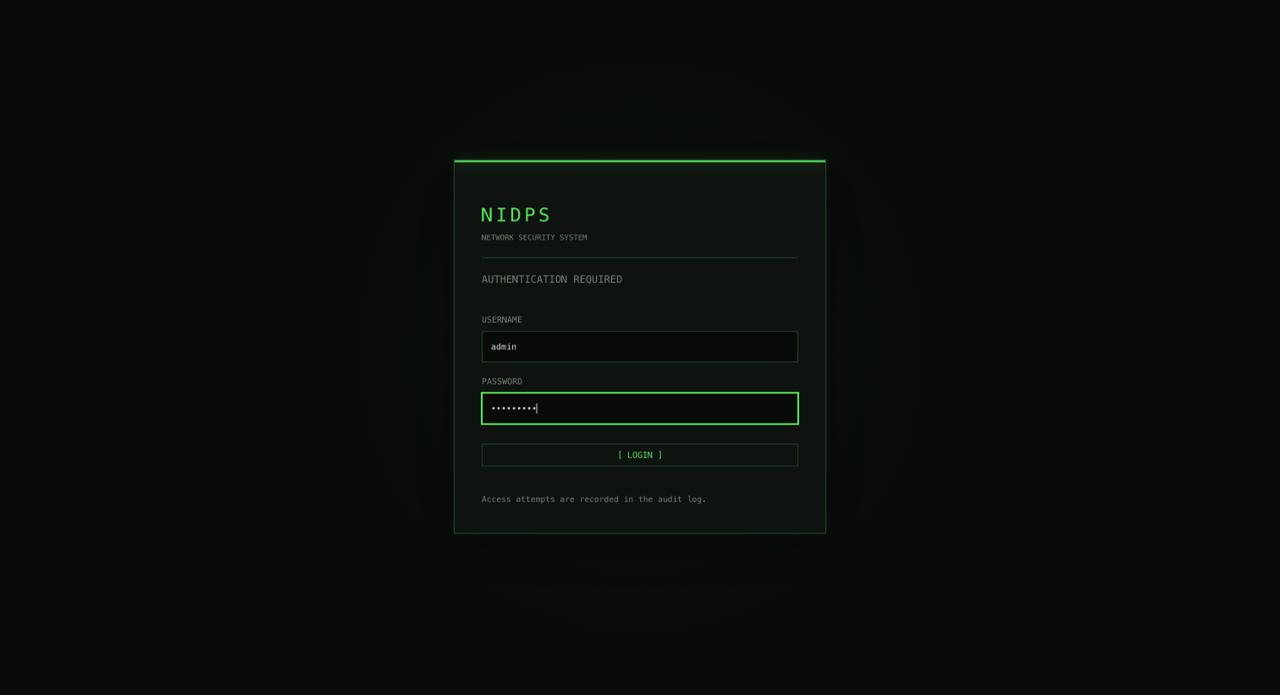
\includegraphics[width=0.89\textwidth,height=0.8\textheight,keepaspectratio]{Figures/gui_login.jpg}
\caption{Login screen.}
\label{fig:4.3}
\end{figure}

\noindent The login screen authenticates the administrator before any information is shown. Error messages do not reveal whether the username or the password was wrong, and the account is locked after repeated failures. Covers: UC-01.

\subsection{Overview Screen}\label{sec:4.8.2}

\begin{figure}[!htbp]
\centering
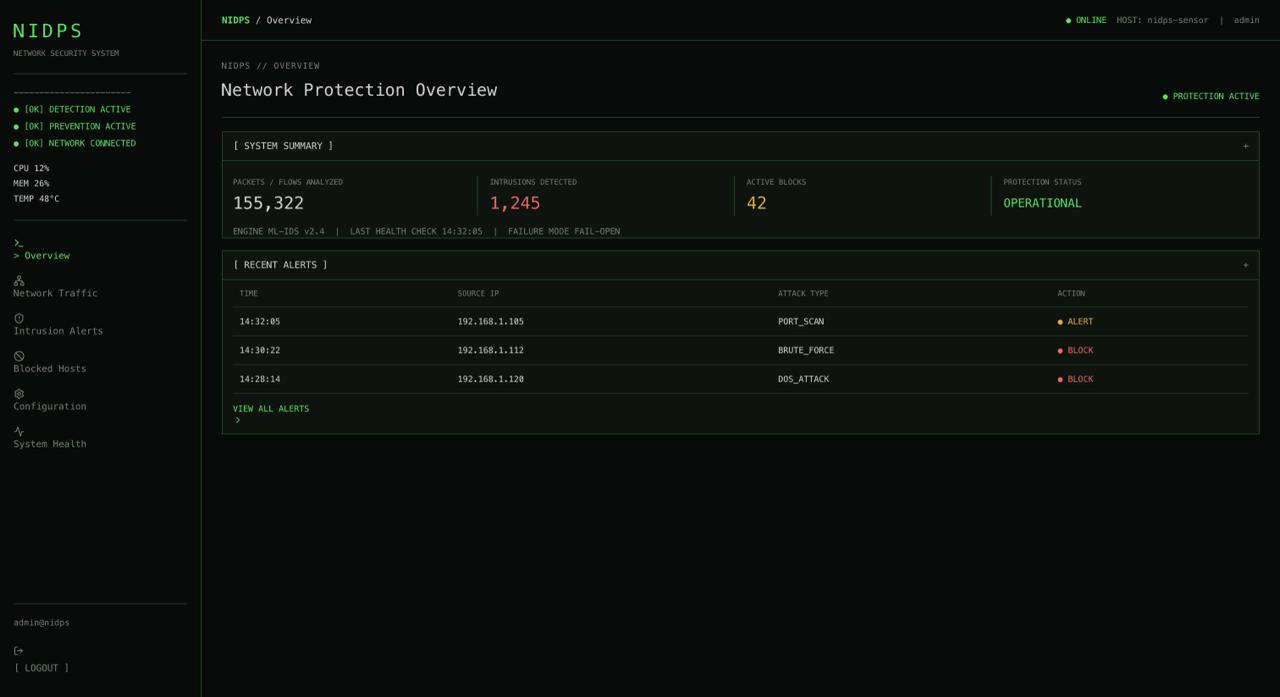
\includegraphics[width=0.99\textwidth,height=0.8\textheight,keepaspectratio]{Figures/gui_overview.jpg}
\caption{Overview screen.}
\label{fig:4.4}
\end{figure}

\noindent The overview screen is the home page. It answers the questions "is my network safe right now?" and "is the NIDPS working?" at a glance. Counters and charts update live. Selecting a device shows its traffic summary and risk history. Covers: UC-02.

\subsection{Alerts Screen}\label{sec:4.8.3}

\begin{figure}[!htbp]
\centering
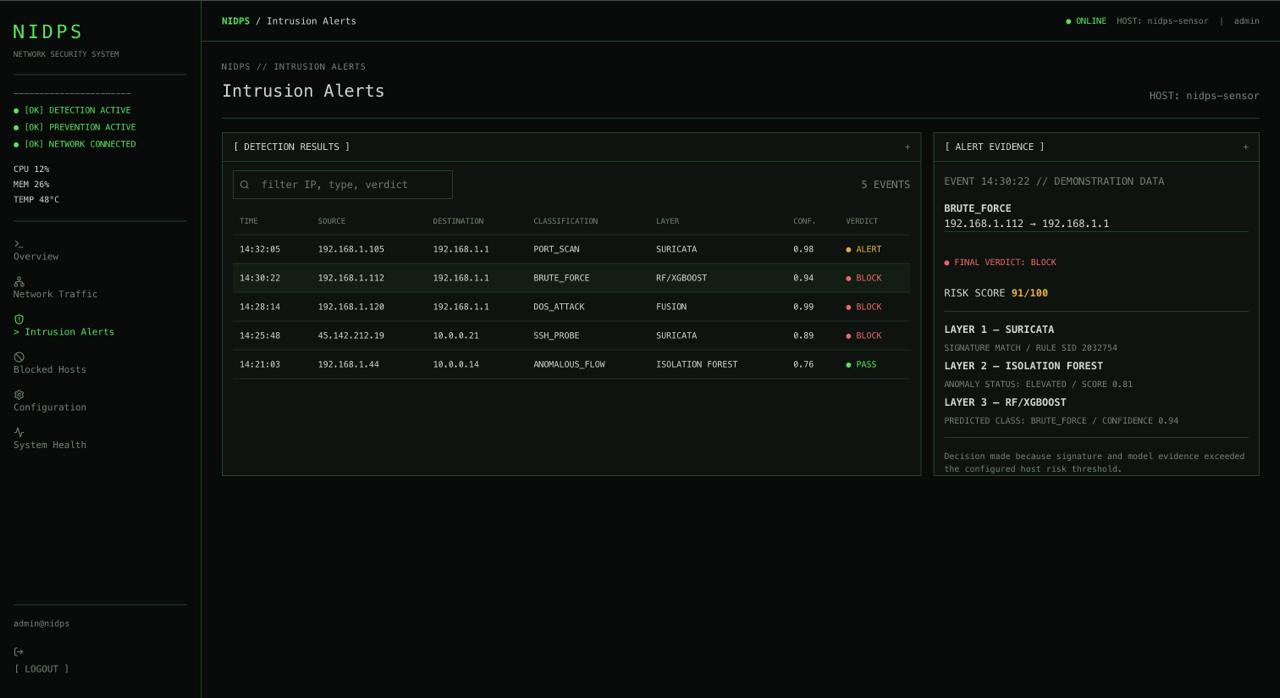
\includegraphics[width=0.99\textwidth,height=0.8\textheight,keepaspectratio]{Figures/gui_alerts.jpg}
\caption{Alerts screen with the evidence panel.}
\label{fig:4.5}
\end{figure}

\noindent The alerts screen lists every ALERT and BLOCK verdict. Selecting an alert opens the evidence panel, which explains in plain language what was detected and shows the evidence from each layer, so the administrator can judge whether the alert is genuine. Covers: UC-03, UC-04 (results).

\subsection{Blocked Hosts and Allowlist Screen}\label{sec:4.8.4}

\begin{figure}[!htbp]
\centering
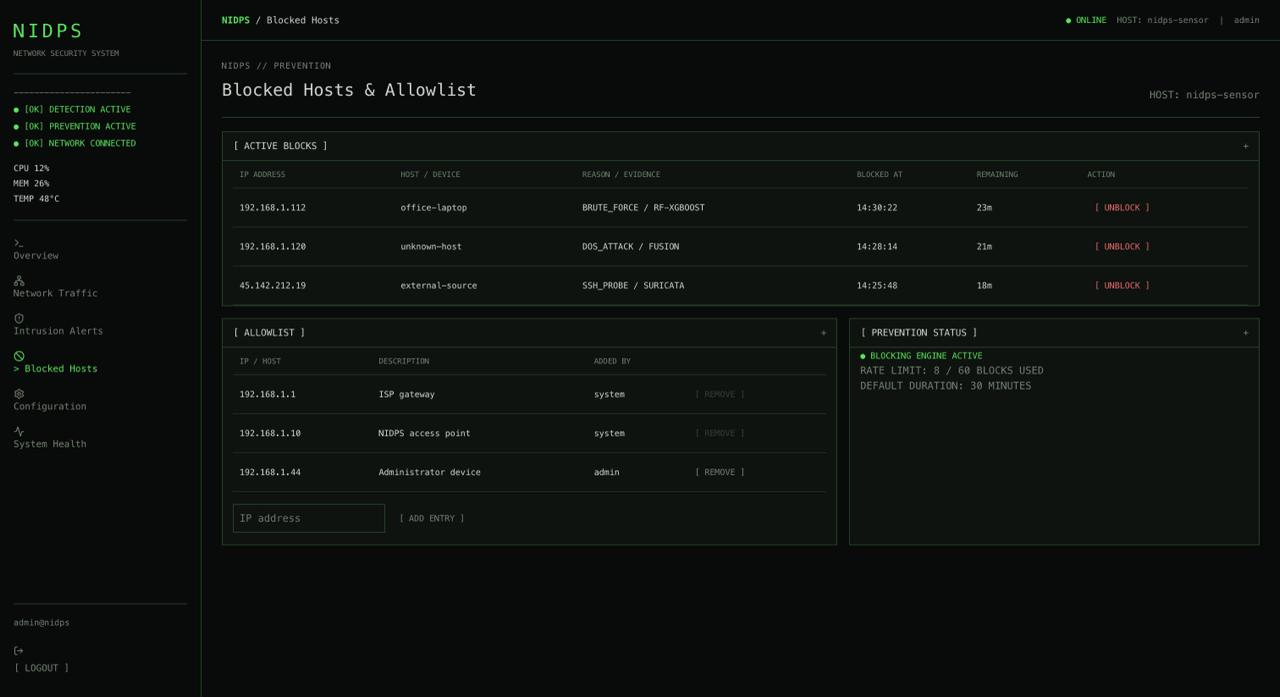
\includegraphics[width=0.99\textwidth,height=0.8\textheight,keepaspectratio]{Figures/gui_blocked.jpg}
\caption{Blocked Hosts and Allowlist screen.}
\label{fig:4.6}
\end{figure}

\noindent This screen lets the administrator see who is blocked and why, release hosts blocked by mistake and maintain the allowlist. A warning banner appears here if the block rate limit has been reached. Covers: UC-05, UC-06.

\subsection{Settings Screen}\label{sec:4.8.5}

\begin{figure}[!htbp]
\centering
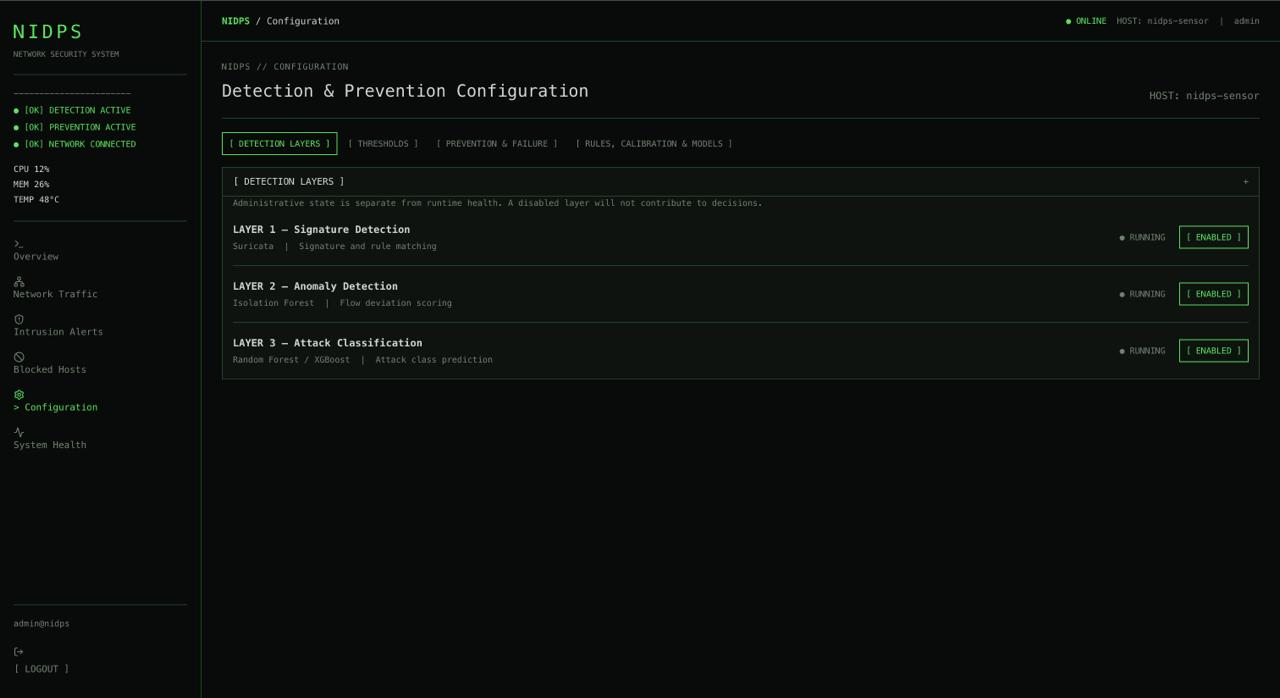
\includegraphics[width=0.99\textwidth,height=0.8\textheight,keepaspectratio]{Figures/gui_settings.jpg}
\caption{Settings screen.}
\label{fig:4.7}
\end{figure}

\noindent The settings screen groups all runtime configuration. Every change is validated, applied without restarting services and recorded in the audit log. Current values are shown next to their defaults. Covers: UC-07, UC-08, UC-09, UC-10, UC-12 (model version display).

\subsection{System Health Screen}\label{sec:4.8.6}

\begin{figure}[H]
\centering
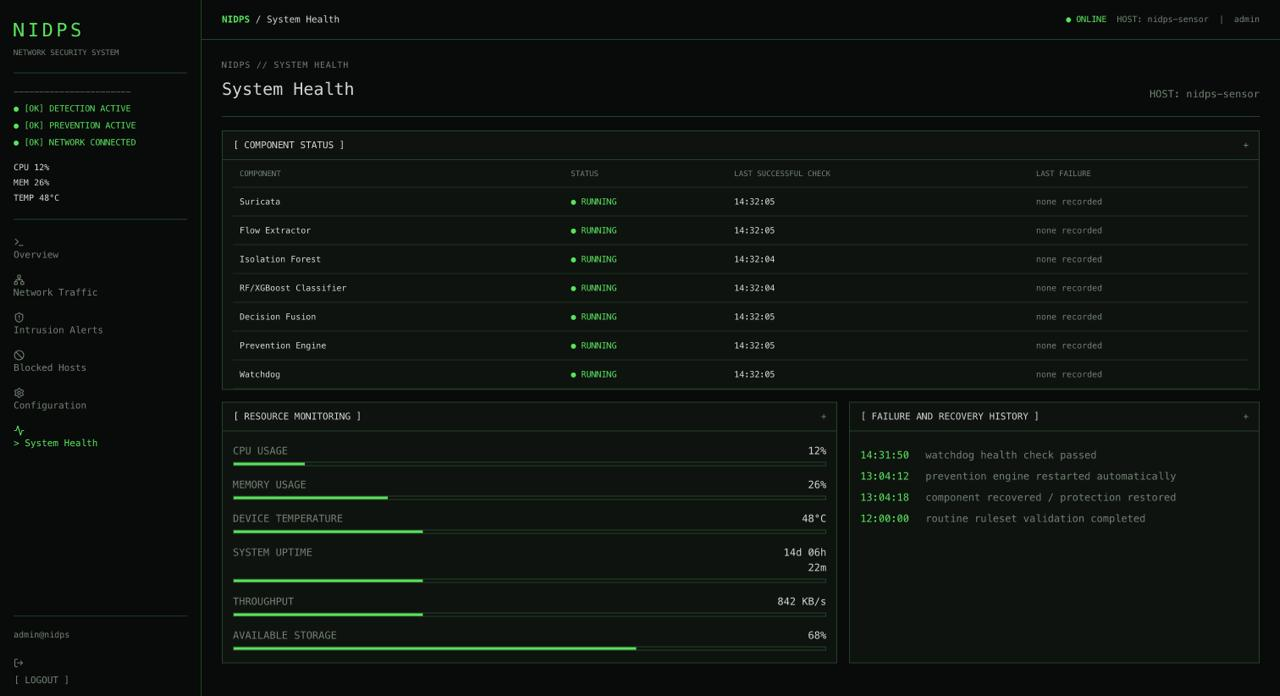
\includegraphics[width=0.99\textwidth,height=0.8\textheight,keepaspectratio]{Figures/gui_health.jpg}
\caption{System Health screen.}
\label{fig:4.8}
\end{figure}

\noindent The health screen shows whether every component is running and how the system has behaved over time, including periods in which it was not fully protecting the network. Covers: UC-11.

\section{Database Design}\label{sec:4.9}

\noindent The NIDPS stores derived data only: hosts, flow records for a short retention window, evidence, verdicts, blocks, the allowlist, model packages, calibration state, configuration, component health events and an audit log. A relational database is used because these records are strongly linked (for example, a block refers to a verdict, which refers to a flow and its evidence) and because the dashboard needs filtered, joined queries. SQLite is chosen because it runs in-process with no server, stores everything in one file and is sufficient for the write rate of a single home device. Raw packets and payloads are never stored. Live counters shown on the dashboard are kept in memory and on the event bus rather than in the database.

\subsection{ER Diagram}\label{sec:4.9.1}

\noindent Figure~\ref{fig:4.9} shows the entity-relationship diagram. HOST is the central entity: a host has many flow records, evidence items, verdicts and blocks. Each flow record can have several evidence items (one per layer) and at most one final verdict, and a BLOCK verdict creates at most one block entry. Evidence produced by an ML layer refers to the model package that produced it, and calibration states belong to the anomaly model. Administrative actions are linked to the admin user who performed them.

\begin{sidewaysfigure}
\centering
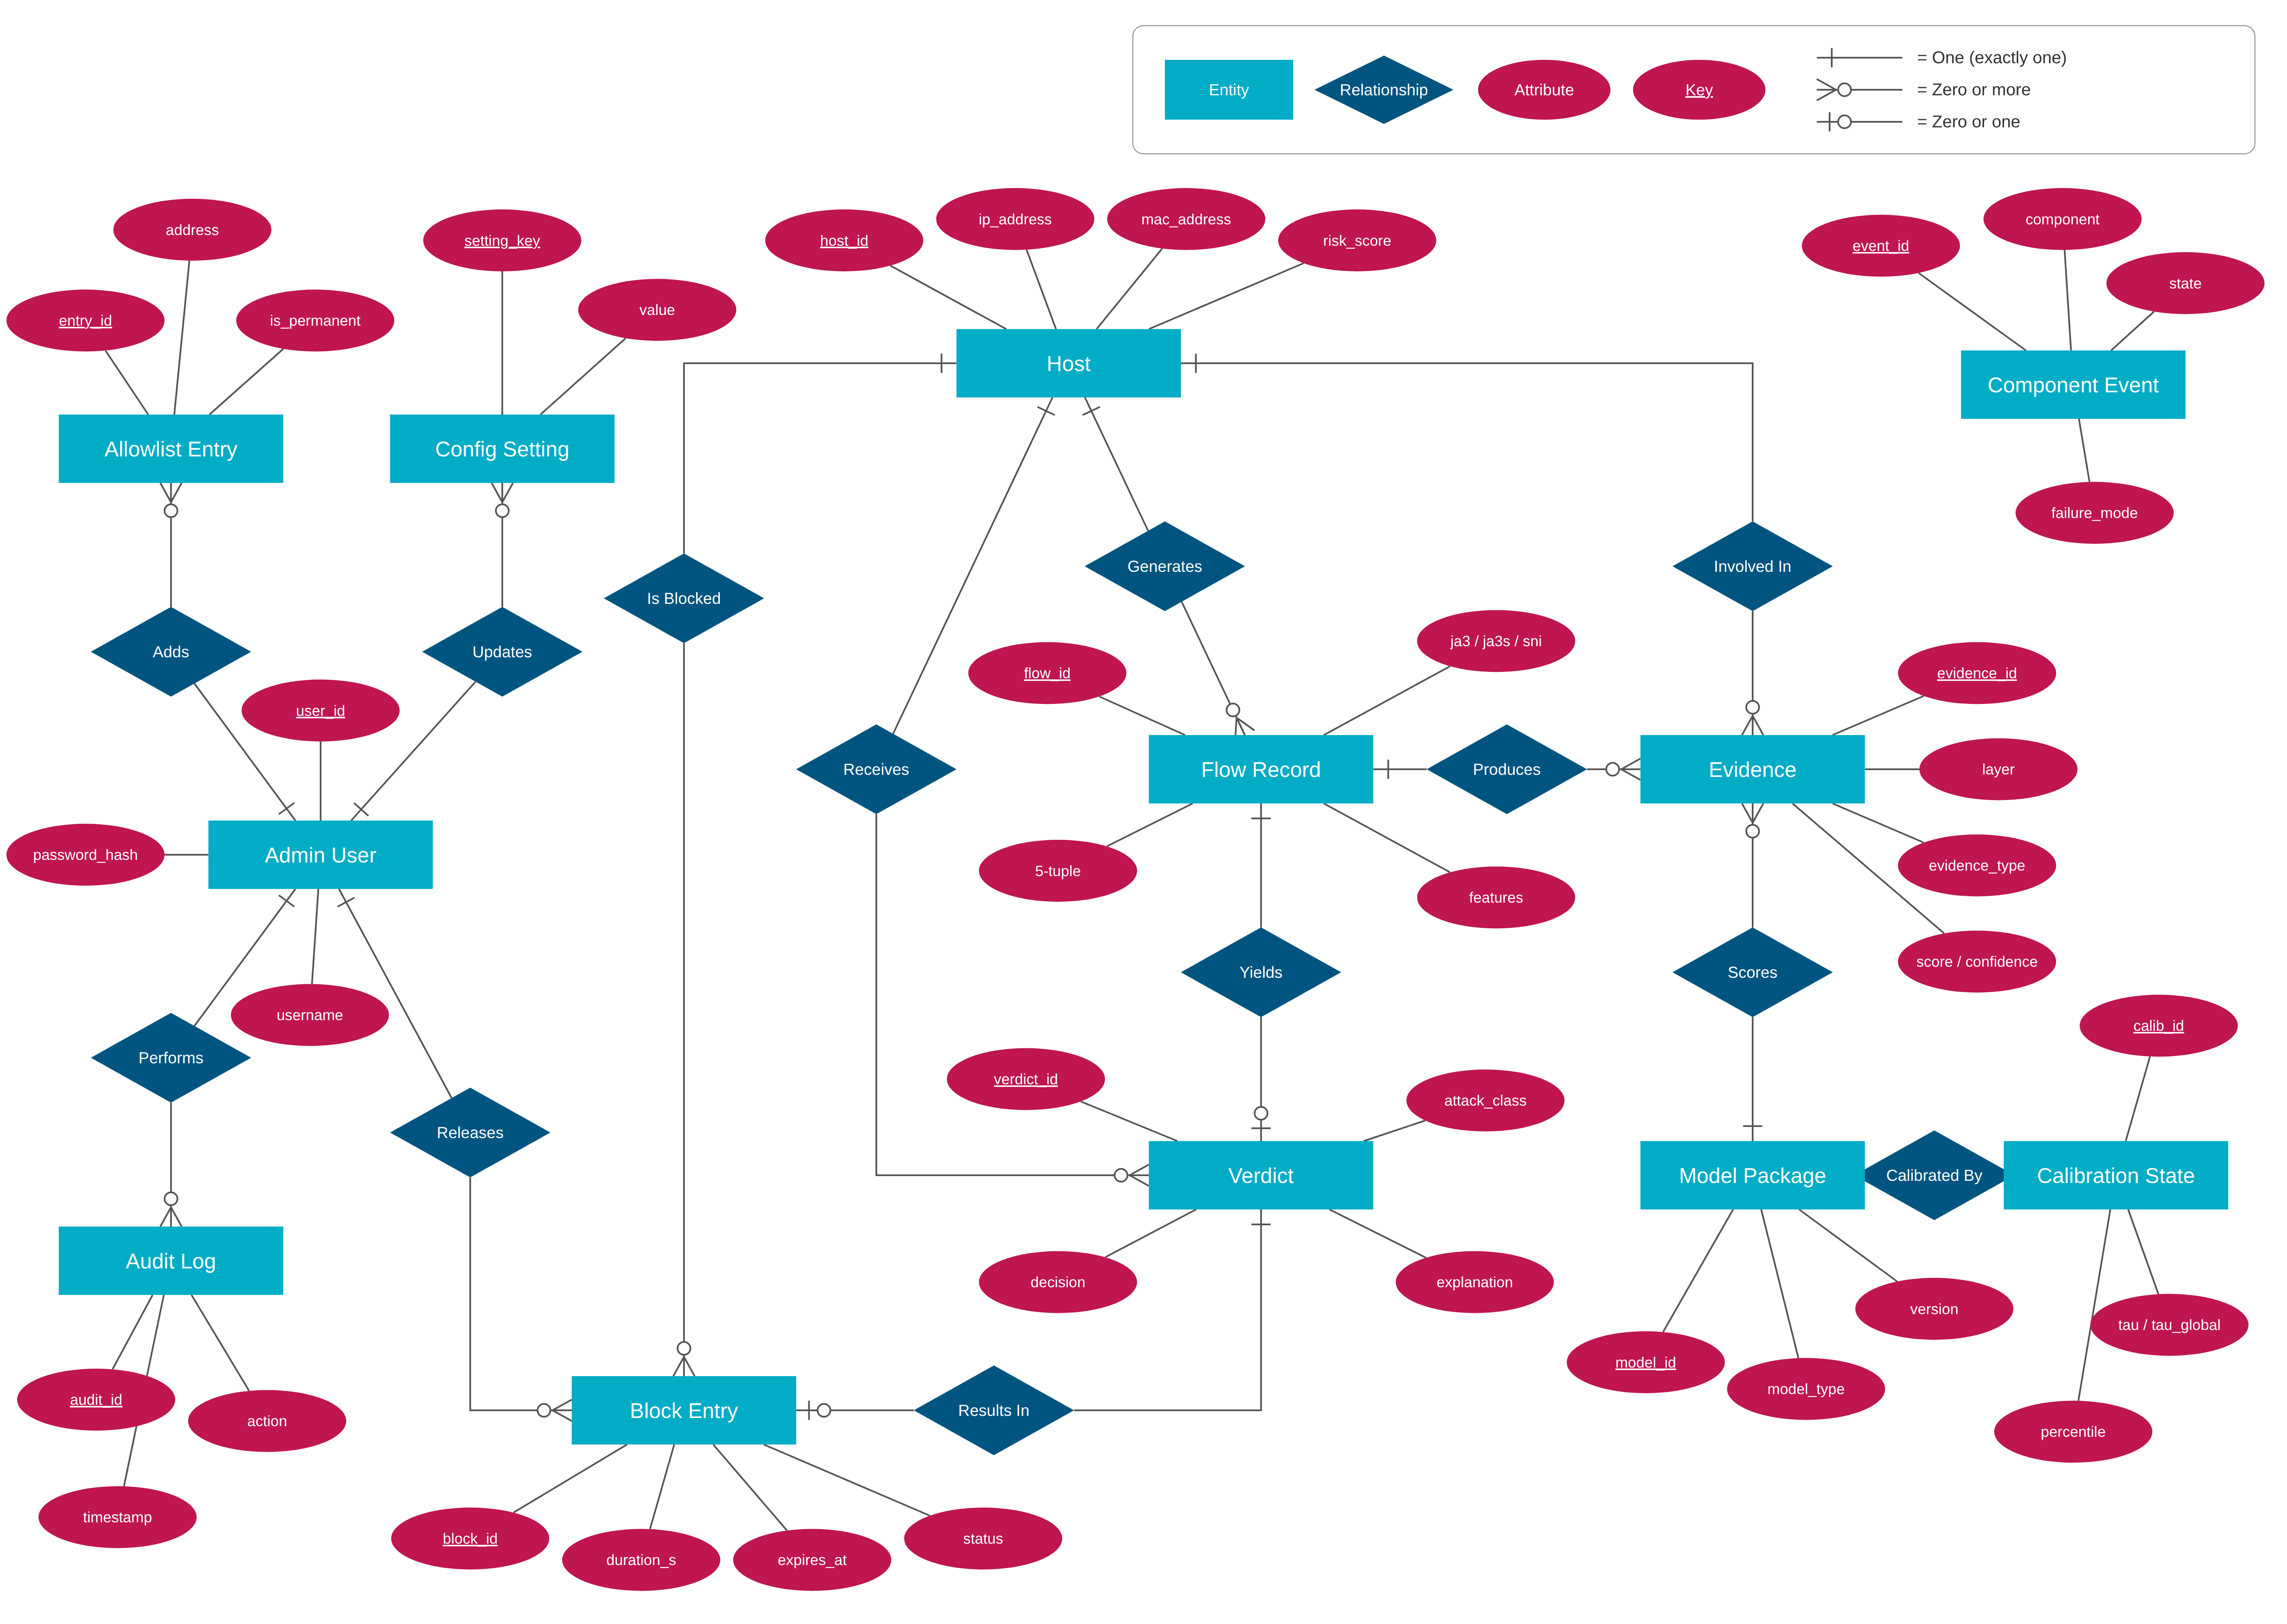
\includegraphics[width=\textheight,height=0.92\textwidth,keepaspectratio]{Figures/nidps_erd_chen.png}
\caption{Entity-relationship diagram of the NIDPS database.}
\label{fig:4.9}
\end{sidewaysfigure}
\FloatBarrier

\subsection{Data Dictionary}\label{sec:4.9.2}

\noindent The tables below describe every entity. PK denotes a primary key and FK a foreign key. Timestamps are stored in UTC in ISO 8601 format.

{\small
\begin{longtable}{|>{\raggedright\arraybackslash}p{\dimexpr 0.279\linewidth-2\tabcolsep-1.3\arrayrulewidth\relax}|>{\raggedright\arraybackslash}p{\dimexpr 0.179\linewidth-2\tabcolsep-1.3\arrayrulewidth\relax}|>{\raggedright\arraybackslash}p{\dimexpr 0.236\linewidth-2\tabcolsep-1.3\arrayrulewidth\relax}|>{\raggedright\arraybackslash}p{\dimexpr 0.306\linewidth-2\tabcolsep-1.3\arrayrulewidth\relax}|}
\caption{Data dictionary for ADMIN\_USER.}\label{tab:4.17}\\
\hline
\textbf{Field} & \textbf{Type} & \textbf{Constraints} & \textbf{Description} \\ \hline
\endfirsthead
\hline
\textbf{Field} & \textbf{Type} & \textbf{Constraints} & \textbf{Description} \\ \hline
\endhead
user\_id & INTEGER & PK & Unique identifier of the administrator \\ \hline
username & TEXT & UNIQUE, NOT NULL & Login name \\ \hline
password\_hash & TEXT & NOT NULL & Salted password hash (e.g. Argon2/bcrypt) \\ \hline
failed\_attempts & INTEGER & DEFAULT 0 & Consecutive failed logins \\ \hline
locked\_until & DATETIME & NULL & End of lock-out period, if locked \\ \hline
created\_at / last\_login & DATETIME &  & Account creation and last successful login \\ \hline
\end{longtable}
}

{\small
\begin{longtable}{|>{\raggedright\arraybackslash}p{\dimexpr 0.279\linewidth-2\tabcolsep-1.3\arrayrulewidth\relax}|>{\raggedright\arraybackslash}p{\dimexpr 0.179\linewidth-2\tabcolsep-1.3\arrayrulewidth\relax}|>{\raggedright\arraybackslash}p{\dimexpr 0.238\linewidth-2\tabcolsep-1.3\arrayrulewidth\relax}|>{\raggedright\arraybackslash}p{\dimexpr 0.304\linewidth-2\tabcolsep-1.3\arrayrulewidth\relax}|}
\caption{Data dictionary for HOST.}\label{tab:4.18}\\
\hline
\textbf{Field} & \textbf{Type} & \textbf{Constraints} & \textbf{Description} \\ \hline
\endfirsthead
\hline
\textbf{Field} & \textbf{Type} & \textbf{Constraints} & \textbf{Description} \\ \hline
\endhead
host\_id & INTEGER & PK & Unique identifier \\ \hline
ip\_address & TEXT & NOT NULL & Current IPv4/IPv6 address \\ \hline
mac\_address & TEXT & NULL & MAC address (internal hosts only) \\ \hline
hostname & TEXT & NULL & Name from DHCP lease or reverse DNS \\ \hline
is\_internal & BOOLEAN & NOT NULL & True if the host is a client of the NIDPS \\ \hline
risk\_score & REAL & DEFAULT 0 & Current decaying evidence score S\_h \\ \hline
first\_seen / last\_seen & DATETIME &  & First and most recent activity \\ \hline
\end{longtable}
}

{\small
\begin{longtable}{|>{\raggedright\arraybackslash}p{\dimexpr 0.282\linewidth-2\tabcolsep-1.3\arrayrulewidth\relax}|>{\raggedright\arraybackslash}p{\dimexpr 0.179\linewidth-2\tabcolsep-1.3\arrayrulewidth\relax}|>{\raggedright\arraybackslash}p{\dimexpr 0.236\linewidth-2\tabcolsep-1.3\arrayrulewidth\relax}|>{\raggedright\arraybackslash}p{\dimexpr 0.304\linewidth-2\tabcolsep-1.3\arrayrulewidth\relax}|}
\caption{Data dictionary for FLOW\_RECORD.}\label{tab:4.19}\\
\hline
\textbf{Field} & \textbf{Type} & \textbf{Constraints} & \textbf{Description} \\ \hline
\endfirsthead
\hline
\textbf{Field} & \textbf{Type} & \textbf{Constraints} & \textbf{Description} \\ \hline
\endhead
flow\_id & INTEGER & PK & Unique identifier \\ \hline
host\_id & INTEGER & FK $\rightarrow$ HOST & Internal host involved in the flow \\ \hline
src\_ip, dst\_ip, src\_port, dst\_port, protocol & TEXT / INTEGER & NOT NULL & 5-tuple (stored for investigation, not used as model features) \\ \hline
start\_time, end\_time & DATETIME & NOT NULL & Flow or segment time span \\ \hline
segment\_no & INTEGER & DEFAULT 0 & Segment number for long flows \\ \hline
ja3, ja3s, sni & TEXT & NULL & TLS fingerprints and server name, if TLS \\ \hline
features & TEXT (JSON) & NOT NULL & 78 flow features \\ \hline
extractor\_version & TEXT & NOT NULL & Version of the flow extractor \\ \hline
\end{longtable}
}

{\small
\begin{longtable}{|>{\raggedright\arraybackslash}p{\dimexpr 0.278\linewidth-2\tabcolsep-1.3\arrayrulewidth\relax}|>{\raggedright\arraybackslash}p{\dimexpr 0.177\linewidth-2\tabcolsep-1.3\arrayrulewidth\relax}|>{\raggedright\arraybackslash}p{\dimexpr 0.246\linewidth-2\tabcolsep-1.3\arrayrulewidth\relax}|>{\raggedright\arraybackslash}p{\dimexpr 0.298\linewidth-2\tabcolsep-1.3\arrayrulewidth\relax}|}
\caption{Data dictionary for EVIDENCE.}\label{tab:4.20}\\
\hline
\textbf{Field} & \textbf{Type} & \textbf{Constraints} & \textbf{Description} \\ \hline
\endfirsthead
\hline
\textbf{Field} & \textbf{Type} & \textbf{Constraints} & \textbf{Description} \\ \hline
\endhead
evidence\_id & INTEGER & PK & Unique identifier \\ \hline
flow\_id & INTEGER & FK $\rightarrow$ FLOW\_RECORD, NULL & Related flow (NULL for ARP or host-level evidence) \\ \hline
host\_id & INTEGER & FK $\rightarrow$ HOST & Host the evidence is about \\ \hline
layer & TEXT & CHECK IN (L1, ARP, L2, L3, HOST) & Detecting layer or host tracker \\ \hline
evidence\_type & TEXT & NOT NULL & e.g. SIGNATURE, ANOMALY, CLASS, EXFIL, BEACON \\ \hline
signature\_id & INTEGER & NULL & Suricata rule SID (Layer 1) \\ \hline
score & REAL & NULL & Anomaly or behaviour score \\ \hline
predicted\_class, confidence & TEXT, REAL & NULL & Layer 3 class and probability \\ \hline
weight & REAL & NOT NULL & Weight w\_v added to host score \\ \hline
model\_id & INTEGER & FK $\rightarrow$ MODEL\_PACKAGE, NULL & Model that produced ML evidence \\ \hline
created\_at & DATETIME & NOT NULL & Time the evidence was produced \\ \hline
\end{longtable}
}

{\small
\begin{longtable}{|>{\raggedright\arraybackslash}p{\dimexpr 0.274\linewidth-2\tabcolsep-1.3\arrayrulewidth\relax}|>{\raggedright\arraybackslash}p{\dimexpr 0.179\linewidth-2\tabcolsep-1.3\arrayrulewidth\relax}|>{\raggedright\arraybackslash}p{\dimexpr 0.243\linewidth-2\tabcolsep-1.3\arrayrulewidth\relax}|>{\raggedright\arraybackslash}p{\dimexpr 0.304\linewidth-2\tabcolsep-1.3\arrayrulewidth\relax}|}
\caption{Data dictionary for VERDICT.}\label{tab:4.21}\\
\hline
\textbf{Field} & \textbf{Type} & \textbf{Constraints} & \textbf{Description} \\ \hline
\endfirsthead
\hline
\textbf{Field} & \textbf{Type} & \textbf{Constraints} & \textbf{Description} \\ \hline
\endhead
verdict\_id & INTEGER & PK & Unique identifier \\ \hline
flow\_id & INTEGER & FK $\rightarrow$ FLOW\_RECORD, NULL & Decided flow (NULL for host-score blocks) \\ \hline
host\_id & INTEGER & FK $\rightarrow$ HOST & Host the verdict applies to \\ \hline
decision & TEXT & CHECK IN (PASS, ALERT, BLOCK) & Verdict \\ \hline
layers & TEXT & NOT NULL & Responsible layer(s), e.g. "L2+L3" \\ \hline
attack\_class & TEXT & NULL & Unified attack class \\ \hline
explanation & TEXT & NOT NULL & Plain-language reason shown on the dashboard \\ \hline
reviewed & BOOLEAN & DEFAULT FALSE & Marked as reviewed by the administrator \\ \hline
created\_at & DATETIME & NOT NULL & Time of the verdict \\ \hline
\end{longtable}
}

{\small
\begin{longtable}{|>{\raggedright\arraybackslash}p{\dimexpr 0.278\linewidth-2\tabcolsep-1.3\arrayrulewidth\relax}|>{\raggedright\arraybackslash}p{\dimexpr 0.179\linewidth-2\tabcolsep-1.3\arrayrulewidth\relax}|>{\raggedright\arraybackslash}p{\dimexpr 0.241\linewidth-2\tabcolsep-1.3\arrayrulewidth\relax}|>{\raggedright\arraybackslash}p{\dimexpr 0.302\linewidth-2\tabcolsep-1.3\arrayrulewidth\relax}|}
\caption{Data dictionary for BLOCK\_ENTRY.}\label{tab:4.22}\\
\hline
\textbf{Field} & \textbf{Type} & \textbf{Constraints} & \textbf{Description} \\ \hline
\endfirsthead
\hline
\textbf{Field} & \textbf{Type} & \textbf{Constraints} & \textbf{Description} \\ \hline
\endhead
block\_id & INTEGER & PK & Unique identifier \\ \hline
host\_id & INTEGER & FK $\rightarrow$ HOST & Blocked host \\ \hline
verdict\_id & INTEGER & FK $\rightarrow$ VERDICT & Verdict that caused the block \\ \hline
offence\_count & INTEGER & NOT NULL & Number of earlier blocks in 24 h (n) \\ \hline
duration\_s & INTEGER & NOT NULL & Block duration D0 $\cdot$ 2\^{}n, capped at D\_max \\ \hline
start\_time, expires\_at & DATETIME & NOT NULL & Start and expiry of the block \\ \hline
status & TEXT & CHECK IN (ACTIVE, EXPIRED, RELEASED, SUPPRESSED) & Current state \\ \hline
released\_by, released\_at & INTEGER, DATETIME & FK $\rightarrow$ ADMIN\_USER, NULL & Manual release details \\ \hline
\end{longtable}
}

{\small
\begin{longtable}{|>{\raggedright\arraybackslash}p{\dimexpr 0.278\linewidth-2\tabcolsep-1.3\arrayrulewidth\relax}|>{\raggedright\arraybackslash}p{\dimexpr 0.179\linewidth-2\tabcolsep-1.3\arrayrulewidth\relax}|>{\raggedright\arraybackslash}p{\dimexpr 0.241\linewidth-2\tabcolsep-1.3\arrayrulewidth\relax}|>{\raggedright\arraybackslash}p{\dimexpr 0.302\linewidth-2\tabcolsep-1.3\arrayrulewidth\relax}|}
\caption{Data dictionary for ALLOWLIST\_ENTRY.}\label{tab:4.23}\\
\hline
\textbf{Field} & \textbf{Type} & \textbf{Constraints} & \textbf{Description} \\ \hline
\endfirsthead
\hline
\textbf{Field} & \textbf{Type} & \textbf{Constraints} & \textbf{Description} \\ \hline
\endhead
entry\_id & INTEGER & PK & Unique identifier \\ \hline
address & TEXT & UNIQUE, NOT NULL & IP or MAC address \\ \hline
description & TEXT &  & Reason, e.g. "Gateway" \\ \hline
is\_permanent & BOOLEAN & DEFAULT FALSE & System entries that cannot be removed \\ \hline
added\_by, added\_at & INTEGER, DATETIME & FK $\rightarrow$ ADMIN\_USER, NULL & Who added it and when \\ \hline
\end{longtable}
}

{\small
\begin{longtable}{|>{\raggedright\arraybackslash}p{\dimexpr 0.283\linewidth-2\tabcolsep-1.3\arrayrulewidth\relax}|>{\raggedright\arraybackslash}p{\dimexpr 0.179\linewidth-2\tabcolsep-1.3\arrayrulewidth\relax}|>{\raggedright\arraybackslash}p{\dimexpr 0.236\linewidth-2\tabcolsep-1.3\arrayrulewidth\relax}|>{\raggedright\arraybackslash}p{\dimexpr 0.302\linewidth-2\tabcolsep-1.3\arrayrulewidth\relax}|}
\caption{Data dictionary for MODEL\_PACKAGE.}\label{tab:4.24}\\
\hline
\textbf{Field} & \textbf{Type} & \textbf{Constraints} & \textbf{Description} \\ \hline
\endfirsthead
\hline
\textbf{Field} & \textbf{Type} & \textbf{Constraints} & \textbf{Description} \\ \hline
\endhead
model\_id & INTEGER & PK & Unique identifier \\ \hline
model\_type & TEXT & CHECK IN (IFOREST, RF, XGB) & Algorithm \\ \hline
version & TEXT & NOT NULL & Semantic version of the package \\ \hline
file\_path & TEXT & NOT NULL & Location in the model registry \\ \hline
feature\_list\_hash, extractor\_version & TEXT & NOT NULL & Schema compatibility information \\ \hline
class\_list & TEXT (JSON) & NULL & Output classes (classifier only) \\ \hline
training\_data, metrics & TEXT (JSON) &  & Datasets used and validation metrics \\ \hline
is\_active & BOOLEAN & NOT NULL & True for the model currently in use \\ \hline
deployed\_at & DATETIME & NOT NULL & Deployment time \\ \hline
\end{longtable}
}

{\small
\begin{longtable}{|>{\raggedright\arraybackslash}p{\dimexpr 0.277\linewidth-2\tabcolsep-1.3\arrayrulewidth\relax}|>{\raggedright\arraybackslash}p{\dimexpr 0.178\linewidth-2\tabcolsep-1.3\arrayrulewidth\relax}|>{\raggedright\arraybackslash}p{\dimexpr 0.245\linewidth-2\tabcolsep-1.3\arrayrulewidth\relax}|>{\raggedright\arraybackslash}p{\dimexpr 0.299\linewidth-2\tabcolsep-1.3\arrayrulewidth\relax}|}
\caption{Data dictionary for CALIBRATION\_STATE.}\label{tab:4.25}\\
\hline
\textbf{Field} & \textbf{Type} & \textbf{Constraints} & \textbf{Description} \\ \hline
\endfirsthead
\hline
\textbf{Field} & \textbf{Type} & \textbf{Constraints} & \textbf{Description} \\ \hline
\endhead
calib\_id & INTEGER & PK & Unique identifier \\ \hline
model\_id & INTEGER & FK $\rightarrow$ MODEL\_PACKAGE & Anomaly model calibrated \\ \hline
tau, tau\_global & REAL & NOT NULL & Calibrated and global thresholds \\ \hline
percentile & REAL & NOT NULL & Percentile p used \\ \hline
sample\_count & INTEGER & NOT NULL & Number of clean flows used \\ \hline
u\_max & INTEGER & NULL & Upload-size limit for exfiltration evidence \\ \hline
window\_start, window\_end, created\_at & DATETIME & NOT NULL & Calibration window and run time \\ \hline
\end{longtable}
}

{\small
\begin{longtable}{|>{\raggedright\arraybackslash}p{\dimexpr 0.275\linewidth-2\tabcolsep-1.3\arrayrulewidth\relax}|>{\raggedright\arraybackslash}p{\dimexpr 0.177\linewidth-2\tabcolsep-1.3\arrayrulewidth\relax}|>{\raggedright\arraybackslash}p{\dimexpr 0.240\linewidth-2\tabcolsep-1.3\arrayrulewidth\relax}|>{\raggedright\arraybackslash}p{\dimexpr 0.307\linewidth-2\tabcolsep-1.3\arrayrulewidth\relax}|}
\caption{Data dictionary for CONFIG\_SETTING.}\label{tab:4.26}\\
\hline
\textbf{Field} & \textbf{Type} & \textbf{Constraints} & \textbf{Description} \\ \hline
\endfirsthead
\hline
\textbf{Field} & \textbf{Type} & \textbf{Constraints} & \textbf{Description} \\ \hline
\endhead
setting\_key & TEXT & PK & e.g. failure\_mode, active\_timeout\_s \\ \hline
value & TEXT & NOT NULL & Current value \\ \hline
default\_value, min\_value, max\_value & TEXT &  & Default and allowed range \\ \hline
updated\_by, updated\_at & INTEGER, DATETIME & FK $\rightarrow$ ADMIN\_USER, NULL & Last change \\ \hline
\end{longtable}
}

{\small
\begin{longtable}{|>{\raggedright\arraybackslash}p{\dimexpr 0.282\linewidth-2\tabcolsep-1.3\arrayrulewidth\relax}|>{\raggedright\arraybackslash}p{\dimexpr 0.179\linewidth-2\tabcolsep-1.3\arrayrulewidth\relax}|>{\raggedright\arraybackslash}p{\dimexpr 0.239\linewidth-2\tabcolsep-1.3\arrayrulewidth\relax}|>{\raggedright\arraybackslash}p{\dimexpr 0.300\linewidth-2\tabcolsep-1.3\arrayrulewidth\relax}|}
\caption{Data dictionary for COMPONENT\_EVENT.}\label{tab:4.27}\\
\hline
\textbf{Field} & \textbf{Type} & \textbf{Constraints} & \textbf{Description} \\ \hline
\endfirsthead
\hline
\textbf{Field} & \textbf{Type} & \textbf{Constraints} & \textbf{Description} \\ \hline
\endhead
event\_id & INTEGER & PK & Unique identifier \\ \hline
component & TEXT & NOT NULL & Service name \\ \hline
state & TEXT & CHECK IN (RUNNING, DEGRADED, FAILED, RECOVERING) & State entered \\ \hline
failure\_mode & TEXT & NULL & Mode applied during the failure \\ \hline
detected\_at, recovered\_at & DATETIME &  & Detection and recovery time \\ \hline
packets\_dropped, packets\_bypassed & INTEGER & DEFAULT 0 & Traffic affected \\ \hline
details & TEXT &  & Cause and diagnostic information \\ \hline
\end{longtable}
}

{\small
\begin{longtable}{|>{\raggedright\arraybackslash}p{\dimexpr 0.272\linewidth-2\tabcolsep-1.3\arrayrulewidth\relax}|>{\raggedright\arraybackslash}p{\dimexpr 0.179\linewidth-2\tabcolsep-1.3\arrayrulewidth\relax}|>{\raggedright\arraybackslash}p{\dimexpr 0.240\linewidth-2\tabcolsep-1.3\arrayrulewidth\relax}|>{\raggedright\arraybackslash}p{\dimexpr 0.309\linewidth-2\tabcolsep-1.3\arrayrulewidth\relax}|}
\caption{Data dictionary for AUDIT\_LOG.}\label{tab:4.28}\\
\hline
\textbf{Field} & \textbf{Type} & \textbf{Constraints} & \textbf{Description} \\ \hline
\endfirsthead
\hline
\textbf{Field} & \textbf{Type} & \textbf{Constraints} & \textbf{Description} \\ \hline
\endhead
audit\_id & INTEGER & PK & Unique identifier \\ \hline
user\_id & INTEGER & FK $\rightarrow$ ADMIN\_USER, NULL & Administrator (NULL for system actions) \\ \hline
action & TEXT & NOT NULL & e.g. LOGIN, BLOCK, RELEASE, CONFIG\_CHANGE \\ \hline
target & TEXT &  & Affected object \\ \hline
old\_value, new\_value & TEXT & NULL & Values before and after a change \\ \hline
timestamp & DATETIME & NOT NULL & Time of the action \\ \hline
\end{longtable}
}

\section{Risk Analysis}\label{sec:4.10}

\noindent The main risks to the project are listed below with their category, likelihood, impact and mitigation. Technical risks concern whether the system can meet its requirements; resource, schedule and project risks concern whether the team can deliver it; legal and ethical risks concern how attack testing is carried out. The risk register is reviewed at every sprint review and updated as risks change.

{\footnotesize\setlength{\tabcolsep}{3.5pt}
\begin{longtable}{|>{\raggedright\arraybackslash}p{\dimexpr 0.073\linewidth-2\tabcolsep-1.3\arrayrulewidth\relax}|>{\raggedright\arraybackslash}p{\dimexpr 0.235\linewidth-2\tabcolsep-1.3\arrayrulewidth\relax}|>{\raggedright\arraybackslash}p{\dimexpr 0.140\linewidth-2\tabcolsep-1.3\arrayrulewidth\relax}|>{\raggedright\arraybackslash}p{\dimexpr 0.133\linewidth-2\tabcolsep-1.3\arrayrulewidth\relax}|>{\raggedright\arraybackslash}p{\dimexpr 0.117\linewidth-2\tabcolsep-1.3\arrayrulewidth\relax}|>{\raggedright\arraybackslash}p{\dimexpr 0.302\linewidth-2\tabcolsep-1.3\arrayrulewidth\relax}|}
\caption{Risk analysis.}\label{tab:4.29}\\
\hline
\textbf{ID} & \textbf{Risk} & \textbf{Category} & \textbf{Likelihood} & \textbf{Impact} & \textbf{Mitigation} \\ \hline
\endfirsthead
\hline
\textbf{ID} & \textbf{Risk} & \textbf{Category} & \textbf{Likelihood} & \textbf{Impact} & \textbf{Mitigation} \\ \hline
\endhead
R1 & Raspberry Pi cannot sustain household throughput with all layers enabled & Technical & Medium & High & Keep ML off the forwarding path; trim rule groups; degraded mode; measure saturation early and switch to a mini-PC if needed. \\ \hline
R2 & Models trained on public datasets perform poorly on real home traffic (dataset shift) & Technical & High & High & Harmonised flow regeneration; per-network threshold calibration; Suricata as a baseline; self-collected test set; report results honestly. \\ \hline
R3 & High false positive rate causes legitimate devices to be blocked & Technical / Business & Medium & High & Fusion requires strong or corroborated evidence; allowlist; rate limit; short first blocks; one-week alert-only soak test before enabling blocking. \\ \hline
R4 & Wireless adapter or driver does not support stable AP mode or client isolation & Technical & Medium & Medium & Test hardware early; use a supported USB adapter; fall back to bridging lateral traffic where needed. \\ \hline
R5 & Encrypted traffic and JA3 randomisation reduce detection coverage & Technical & High & Medium & Rely on flow metadata; combine JA3 with JA3S and SNI; isolate fingerprinting so JA4 can be adopted. \\ \hline
R6 & Errors in public dataset labels or flow construction distort training & Technical & Medium & Medium & Regenerate flows from raw PCAPs; relabel from attack schedules; prefer corrected dataset versions where available. \\ \hline
R7 & Large dataset PCAPs exceed available storage or memory for training & Resource & Medium & Medium & Process captures in chunks; sample benign traffic; use external storage or university lab machines. \\ \hline
R8 & The NIDPS becomes a single point of failure and causes network outages & Operational & Low & High & Kernel-enforced fail-open default; watchdog; automatic restarts; timed blocks. \\ \hline
R9 & An attacker poisons calibration or evades the models & Security & Low & High & Exclude flagged flows from calibration; bound threshold shift; no online retraining; signatures remain active. \\ \hline
R10 & Attack experiments affect devices or networks outside the project & Legal / Ethical & Low & High & Run attacks only on an isolated lab network owned by the team; capture only the team's own traffic. \\ \hline
R11 & Schedule slippage due to integration complexity of many services & Schedule & Medium & Medium & Incremental delivery of vertical slices; Layer 1 delivered first; sprint reviews with the supervisor. \\ \hline
R12 & Hardware damage or failure (SD card corruption, overheating) & Resource & Medium & Medium & Use quality storage and cooling; keep image backups; keep a spare SD card. \\ \hline
R13 & Team member unavailability & Project & Low & Medium & Shared repository and documentation; pair work on critical components; clear task ownership. \\ \hline
\end{longtable}
}

\noindent The two risks rated most serious are R2 and R3, because they determine whether the system is useful on a real network. Both are addressed by design (harmonised features, local calibration and cautious decision fusion) and are measured directly in the evaluation, so that their real effect is known rather than assumed.

\chapter{Proposed Approach and Methodology}\label{chap:5}
\label{chap:approach}
\noindent This chapter presents the methodology through which the proposed Network Intrusion Detection and Prevention System (NIDPS) detects and blocks malicious traffic on a small network. The proposed approach is a hybrid detection framework: three complementary detection layers, a decision-fusion algorithm that turns their outputs into a single verdict, and an enforcement and recovery mechanism that acts on that verdict. The chapter begins with the datasets and the way they are harmonised so that models trained offline see the same features at runtime. It then walks through the backend algorithms that are not visible in the system design: flow construction, TLS fingerprinting, rule-based detection, Isolation Forest scoring with per-network threshold calibration, supervised attack classification, verdict fusion, automated blocking and the failure-handling state machine. The chapter closes with the evaluation protocol used to measure detection quality and the behaviour of the system on constrained hardware.

\section{Overview of the Proposed Framework}\label{sec:5.1}
\label{sec:overview}
\noindent The NIDPS runs on a single Linux host that acts as the network's wireless access point, so every packet between client devices and the ISP gateway passes through it. Each packet travels two paths at once. On the inline path, Suricata inspects packets as they are forwarded and can drop them immediately. On the analysis path, packets are grouped into bidirectional flows, and each completed flow is described by 78 statistical features plus TLS fingerprints (JA3/JA3S). These flow records are scored by an unsupervised Isolation Forest (Layer~2) and a supervised Random Forest/XGBoost classifier (Layer~3).

\noindent The three layers cover different threat classes:
\begin{itemize}
    \item \textbf{Layer 1 -- Signature detection (Suricata):} known attacks with stable signatures, such as SSH brute force, port scanning and DNS spoofing.
    \item \textbf{Layer 2 -- Anomaly detection (Isolation Forest):} traffic that deviates from the network's normal profile, including zero-day behaviour, C2 beaconing and data exfiltration.
    \item \textbf{Layer 3 -- Supervised classification (Random Forest/XGBoost):} assignment of suspicious flows to known attack families such as DDoS and lateral movement.
\end{itemize}

\noindent A decision-fusion engine combines the three outputs into one verdict per flow (pass, alert or block). Block verdicts are enforced through iptables and ipset. A watchdog supervises every component and applies the configured failure mode when one of them stops. Figure~\ref{fig:pipeline} summarises this pipeline.

\begin{figure}[!htbp]
    \centering
    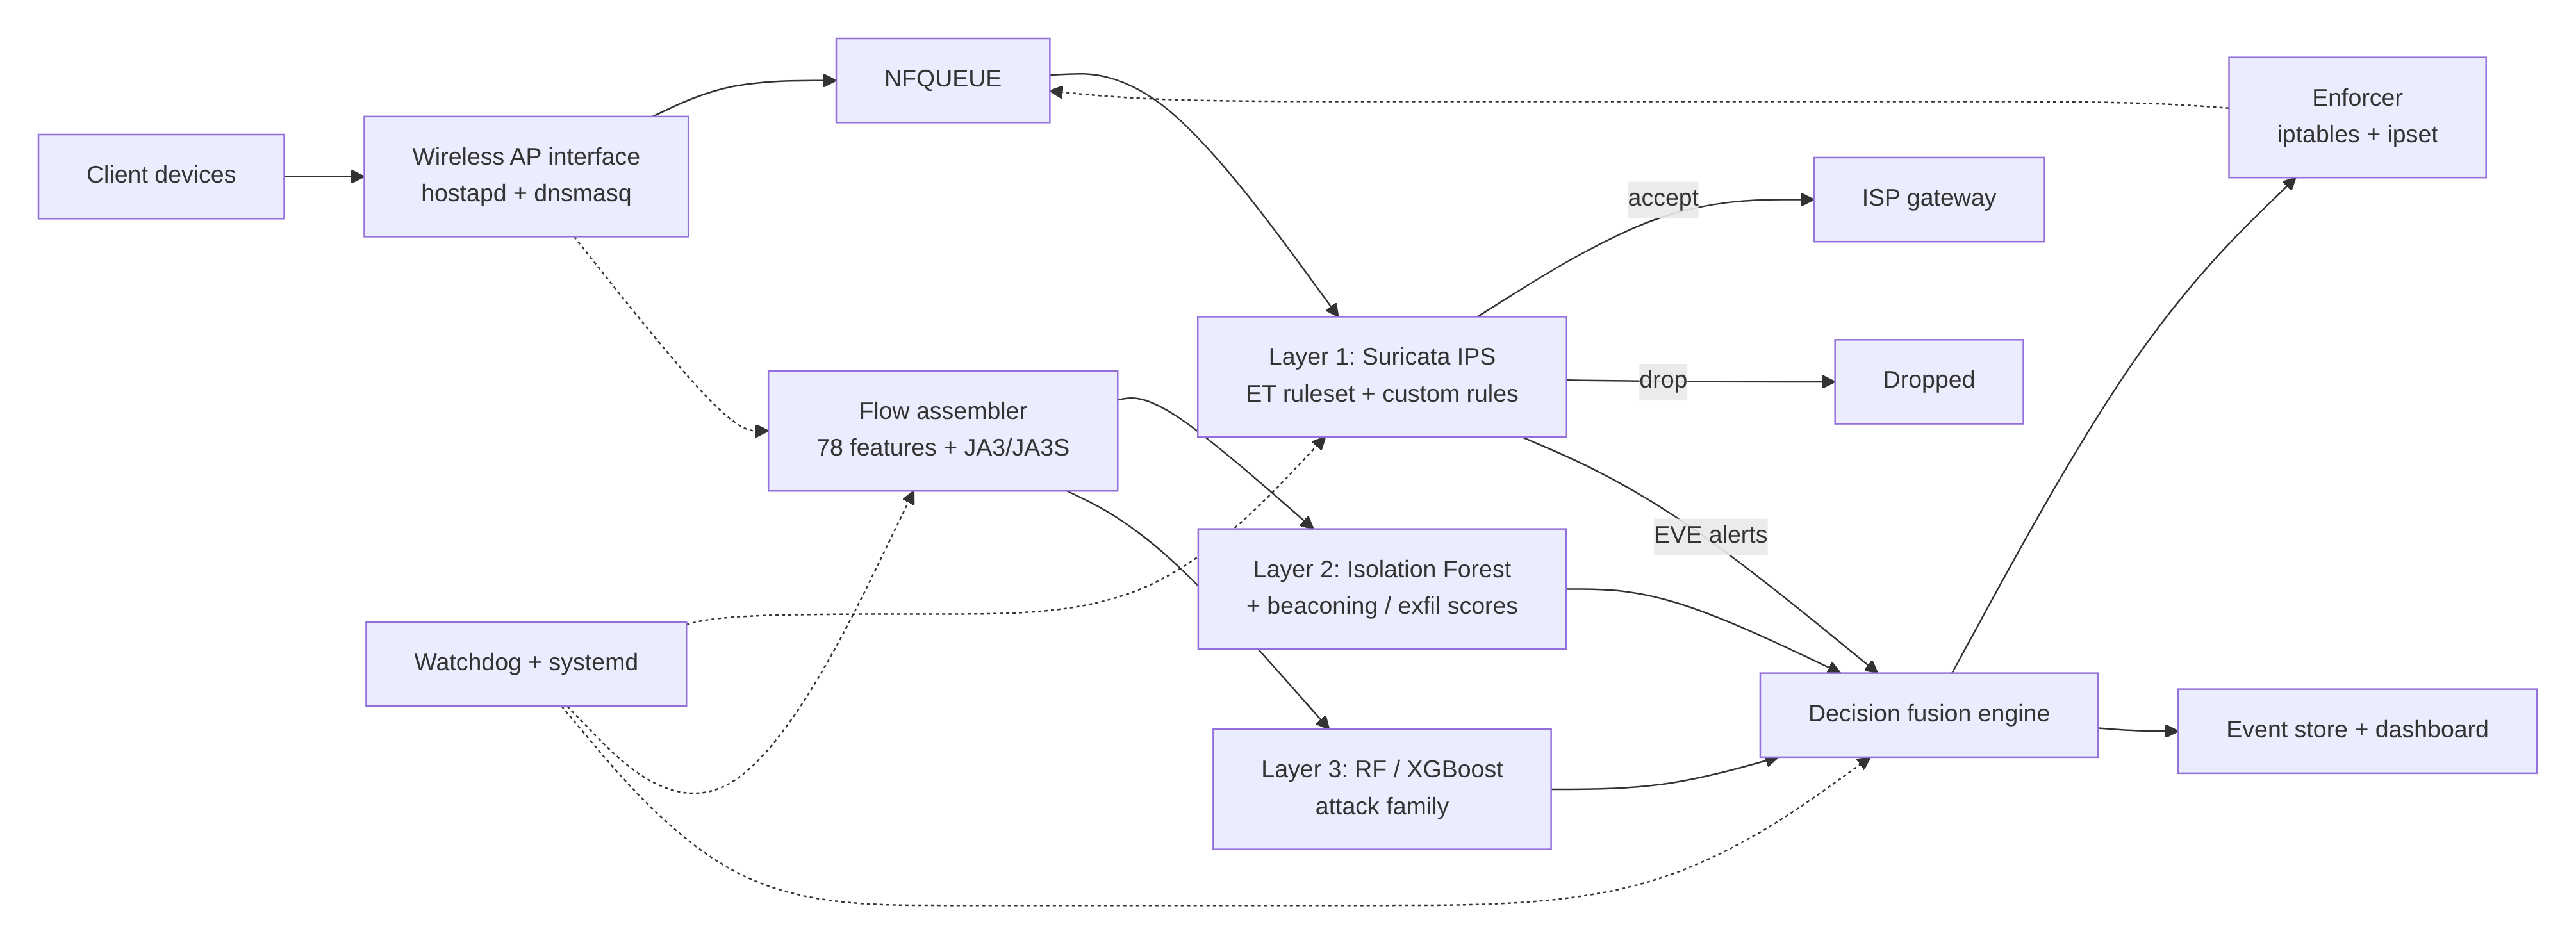
\includegraphics[width=\textwidth]{Figures/nidps_fig5_1.png}
    \caption{Proposed three-layer NIDPS pipeline.}
    \label{fig:pipeline}
\end{figure}

\noindent The design separates what must be fast from what can be thorough. Suricata decides per packet and adds only microseconds of forwarding delay. The machine learning layers decide per flow, so their verdicts are applied to the remainder of a long flow and to all later traffic from the offending host.

\section{Datasets}\label{sec:5.2}
\label{sec:datasets}
\noindent The machine learning layers are trained on three public intrusion detection benchmarks and evaluated additionally on traffic captured from our own deployment. The goal is not the highest score on one benchmark, but a model that still works when the training traffic and the deployment traffic differ.

\subsection{Public Benchmark Datasets}\label{sec:5.2.1}
\label{sec:public-datasets}
\noindent Table~\ref{tab:datasets} lists the public datasets used for training and cross-evaluation.

\begin{table}[H]
\centering
\caption{Public benchmark datasets used for training and cross-evaluation.}
\label{tab:datasets}
\begin{tabular}{|>{\raggedright\arraybackslash}p{0.17\linewidth}|>{\raggedright\arraybackslash}p{0.17\linewidth}|>{\raggedright\arraybackslash}p{0.22\linewidth}|>{\raggedright\arraybackslash}p{0.30\linewidth}|}
\hline
\textbf{Dataset} & \textbf{Source} & \textbf{Traffic profile} & \textbf{Attack families relevant to this project} \\
\hline
CIC-IDS-2017 \cite{nidps:cicids2017} & Canadian Institute for Cybersecurity (CIC) & 5 days of enterprise-style traffic & Brute force (SSH/FTP), DoS/DDoS, port scan, botnet, infiltration \\
\hline
CSE-CIC-IDS2018 \cite{nidps:cicids2018} & CIC with the Communications Security Establishment & Larger AWS-hosted network, 10 days & Brute force, DoS/DDoS, botnet, infiltration \\
\hline
CIC-IoT-2023 \cite{nidps:ciciot2023} & CIC & 105 IoT devices in a smart-home topology & DDoS, recon/scan, spoofing, brute force, Mirai-style attacks \\
\hline
\end{tabular}
\end{table}

\noindent CIC-IoT-2023 is closest to the target environment because home networks are increasingly dominated by IoT devices. CIC-IDS-2017 and CSE-CIC-IDS2018 contribute a wider range of host-based attacks. Published analyses of CIC-IDS-2017 have reported labelling and flow-construction errors in the original CSV files \cite{nidps:engelen2021}, which is one more reason flows are regenerated from the raw captures (Section~\ref{sec:harmonisation}).

\subsection{Self-Collected Real-World Dataset}\label{sec:5.2.2}
\label{sec:selfcollected}
\noindent A fourth dataset is captured on the deployed access point itself. It has two parts:
\begin{enumerate}
    \item \textbf{Benign capture.} Normal household or lab traffic (browsing, streaming, video calls, IoT devices, software updates) is recorded over several days. Flows that Suricata flags during this period are removed before the capture is labelled benign.
    \item \textbf{Attack capture.} Each in-scope attack is executed from a dedicated attacker machine in an isolated test network that we own, using standard penetration-testing tools. The start and end time, attacker address and target of each run are logged, so every flow in the window can be labelled automatically from these logs.
\end{enumerate}
\noindent This dataset is used only for testing, never for training. It measures how well models trained on public data transfer to a real home network.

\subsection{Feature Harmonisation Across Datasets}\label{sec:5.2.3}
\label{sec:harmonisation}
\noindent The public datasets do not share one feature format. The two CIC-IDS sets ship CICFlowMeter CSVs with about 80 columns whose names and rounding differ between releases, while CIC-IoT-2023 ships a different, smaller feature set computed over packet windows. A model trained on one format cannot be applied to another, and none of them is guaranteed to match what the live system computes.

\noindent To remove this mismatch, the following procedure is applied:
\begin{enumerate}
    \item Download the raw PCAP files of every dataset instead of the provided CSVs.
    \item Run the same flow extractor that runs on the device (Section~\ref{sec:flowassembly}) over every PCAP. All datasets then share an identical 78-feature schema, with identical definitions, timeouts and units. The extractor runs with the same timeouts as the device ($T_a = 10$\,s, $T_i = 30$\,s), so a training record and a live record always cover the same span of traffic.
    \item Re-label the regenerated flows by matching their 5-tuple and timestamps against each dataset's published attack schedule.
    \item Map every dataset-specific label onto one unified attack taxonomy (Table~\ref{tab:taxonomy}).
\end{enumerate}
\noindent The key advantage is that training-time and serving-time features are produced by the same code, so there is no train/serve skew.

\begin{table}[H]
\centering
\caption{Unified attack taxonomy used for Layer 3.}
\label{tab:taxonomy}
\begin{tabular}{|>{\raggedright\arraybackslash}p{0.24\linewidth}|>{\raggedright\arraybackslash}p{0.46\linewidth}|>{\raggedright\arraybackslash}p{0.16\linewidth}|}
\hline
\textbf{Unified class} & \textbf{Examples of original labels} & \textbf{Primary detecting layer} \\
\hline
Benign & BENIGN, BenignTraffic & -- \\
\hline
Reconnaissance & PortScan, Recon-PortScan, Recon-OSScan & L1, L3 \\
\hline
Brute force & SSH-Patator, FTP-Patator, DictionaryBruteForce & L1, L3 \\
\hline
DoS / DDoS & DoS Hulk, DDoS LOIC, DDoS-SYN\_Flood, DDoS-UDP\_Flood & L1, L3 \\
\hline
Botnet / C2 & Bot, Mirai variants & L2, L3 \\
\hline
Spoofing & DNS\_Spoofing, MITM-ArpSpoofing & L1 \\
\hline
Infiltration / lateral movement & Infiltration, internal scanning after compromise & L3 \\
\hline
\end{tabular}
\end{table}

\subsection{Pre-processing}\label{sec:5.2.4}
\label{sec:preprocessing}
\noindent The regenerated flow tables are cleaned before training:
\begin{itemize}
    \item \textbf{Invalid values:} rows with infinite or undefined values (for example, rates computed over a zero-length flow) are dropped, and exact duplicate rows are removed.
    \item \textbf{Identifier removal:} source and destination IP addresses, ports, flow IDs and timestamps are removed from the feature vector. They identify the lab, not the attack, and keeping them lets a model memorise the attacker's address instead of learning behaviour.
    \item \textbf{Constant features:} features with zero variance in the training set are removed.
    \item \textbf{Splitting:} within one dataset, the split into training and test sets is done by capture day rather than at random, because neighbouring flows of the same attack run are nearly identical and a random split leaks them into both sets.
    \item \textbf{Class imbalance:} class proportions are heavily skewed, in opposite directions: benign flows dominate CIC-IDS-2017, while attack flows dominate CIC-IoT-2023. Layer 3 uses class weights inversely proportional to class frequency; oversampling (SMOTE), if used, is applied only to the training fold.
    \item \textbf{Scaling:} tree-based models do not need feature scaling, so values are kept in their original units. This also keeps the online pipeline simple.
    \item \textbf{Isolation Forest training set:} Layer 2 is trained only on benign flows, since it models normal behaviour.
\end{itemize}

\section{Traffic Acquisition and Flow Construction}\label{sec:5.3}
\label{sec:acquisition}
\noindent All detection depends on how packets reach the detectors and how they are summarised. This section describes the inline packet path, the flow assembly algorithm and the extraction of TLS fingerprints from encrypted traffic.

\subsection{Inline Packet Path}\label{sec:5.3.1}
\label{sec:packetpath}
\noindent The host runs hostapd to expose a wireless network and dnsmasq to provide DHCP and DNS to clients. IP forwarding is enabled and the uplink interface performs NAT towards the ISP gateway. Forwarded traffic is diverted by an iptables rule in the FORWARD chain to an NFQUEUE, where Suricata runs in IPS mode. For each packet, Suricata returns an accept or drop verdict to the kernel.

\noindent A copy of every forwarded packet is also read by the flow assembler through a packet capture socket on the wireless interface. The flow assembler never holds packets back, so a slow ML layer cannot slow down forwarding.

\noindent One platform detail matters for lateral movement. By default, the wireless driver and hostapd relay frames between two wireless clients directly, without passing them up to the IP layer, so netfilter and Suricata never see them. To inspect client-to-client traffic, client isolation (\texttt{ap\_isolate=1}) is enabled and intra-network traffic is routed through the host. Without this setting, lateral movement can only be detected when it crosses the AP's IP layer.

\subsection{Flow Assembly Algorithm}\label{sec:5.3.2}
\label{sec:flowassembly}
\noindent A flow is the set of packets sharing the same 5-tuple (source IP, destination IP, source port, destination port, protocol) in either direction. The direction of the first packet defines ``forward''; replies are ``backward''. Algorithm~\ref{alg:flow} shows how flows are built and closed.

\begin{algorithm}[H]
\caption{Bidirectional flow assembly}
\label{alg:flow}
\KwIn{packet stream $P$; active timeout $T_a$ (default 10\,s); idle timeout $T_i$ (default 30\,s)}
\KwOut{completed flow records with 78 features}
$FlowTable \leftarrow$ empty hash map keyed by canonical 5-tuple\;
\ForEach{packet $p \in P$}{
    $k \leftarrow \mathrm{canonical}(p.\mathrm{5tuple})$ \tcp*{same key for both directions}
    \If{$k \notin FlowTable$}{
        create flow $f$ with $f.start \leftarrow p.time$ and $f.fwd \leftarrow$ direction of $p$\;
        $FlowTable[k] \leftarrow f$\;
    }
    $f \leftarrow FlowTable[k]$\;
    update the running statistics of $f$ with $p$ (direction, size, flags, time)\;
    \If{$p$ carries a TLS ClientHello or ServerHello}{
        attach JA3/JA3S to $f$ (Algorithm~\ref{alg:ja3})\;
    }
    \uIf{$p$ has FIN in both directions or RST}{
        emit($f$)\; remove $k$\;
    }
    \ElseIf{$p.time - f.start \geq T_a$}{
        emit($f$) as a partial record\; reset the counters of $f$ but keep $k$\;
    }
}
\tcp{run periodically}
\ForEach{flow $f$ with $now - f.last\_seen \geq T_i$}{
    emit($f$)\; remove its key\;
}
\end{algorithm}

\noindent The active timeout lets a long-running connection, such as a slow exfiltration channel, be scored in segments while it is still open, instead of only when it closes. Each segment is emitted as its own flow record, after which its counters reset. The idle timeout reclaims memory from flows that stop without a FIN or RST. Table~\ref{tab:timeouts} gives the default values.

\begin{table}[H]
\centering
\caption{Flow timeout parameters.}
\label{tab:timeouts}
\begin{tabular}{|>{\raggedright\arraybackslash}p{0.22\linewidth}|>{\raggedright\arraybackslash}p{0.24\linewidth}|>{\raggedright\arraybackslash}p{0.42\linewidth}|}
\hline
\textbf{Parameter} & \textbf{Default} & \textbf{Effect} \\
\hline
Active timeout $T_a$ & 10\,s (configurable, e.g.\ 5--30\,s) & An open flow is re-scored every $T_a$, which caps how long one connection can run unscored \\
\hline
Idle timeout $T_i$ & 30\,s & A flow with no packets for $T_i$ is closed and scored \\
\hline
\end{tabular}
\end{table}

\noindent Most flows, such as web requests, DNS lookups and scan probes, end in well under 5 seconds and are scored once, when they close. Only long-lived connections are segmented. $T_a$ trades CPU for reaction time: halving it doubles the scoring work for long flows. The default of 10\,s is a conservative starting point for low-cost hardware. $T_a$ is a configuration parameter, so a deployment with spare CPU can lower it, for example to 5\,s, to react faster. The evaluation measures both settings (Section~\ref{sec:sysperf}).

\noindent The 78 features follow the CICFlowMeter definitions: packet and byte counts per direction, packet length statistics, inter-arrival time statistics, TCP flag counts, header lengths, bulk and sub-flow measures, and active/idle periods. To keep memory constant per flow, means and variances are updated incrementally with Welford's method (Equation~\ref{eq:welford}) rather than by storing every packet:
\begin{equation}
\label{eq:welford}
\begin{aligned}
\mu_n &= \mu_{n-1} + \frac{x_n - \mu_{n-1}}{n}, \\
M_n &= M_{n-1} + (x_n - \mu_{n-1})(x_n - \mu_n), \\
\sigma_n^2 &= \frac{M_n}{n-1}.
\end{aligned}
\end{equation}
\noindent Here $x_n$ is the $n$-th observation (for example, a packet length), $\mu_n$ the running mean and $M_n$ the running sum of squared deviations. Minimum and maximum are tracked directly.

\subsection{TLS Fingerprint Extraction (JA3/JA3S)}\label{sec:5.3.3}
\label{sec:ja3}
\noindent Most traffic is encrypted, so payload cannot be inspected without decryption. Decrypting traffic on the AP would require installing a certificate on every client, would break certificate pinning in many apps and would cost far more CPU than the target hardware can spare. Instead, the system uses fields of the TLS handshake that are sent in clear text \cite{nidps:ja3}, as shown in Algorithm~\ref{alg:ja3}.

\begin{algorithm}[H]
\caption{JA3/JA3S fingerprint}
\label{alg:ja3}
\KwIn{TLS ClientHello (or ServerHello)}
\KwOut{32-character MD5 fingerprint}
read the TLS version, cipher suites, extension types, supported groups (elliptic curves) and EC point formats\;
remove GREASE values (0x0a0a, 0x1a1a, \ldots, 0xfafa) from every list\;
join the decimal values of each list with ``-''\;
$s_{JA3} \leftarrow$ Version,Ciphers,Extensions,Groups,PointFormats\;
$s_{JA3S} \leftarrow$ Version,Cipher,Extensions \tcp*{ServerHello}
\Return{MD5($s$)}\;
\end{algorithm}

\noindent The fingerprint identifies the client software that opened the connection, not the user. Malware and C2 frameworks often use TLS libraries with fingerprints that differ from common browsers and operating systems. The pair (JA3, JA3S) is attached to the flow record and used by Layer 2 in two ways: as a rarity signal (how many local hosts have ever used this fingerprint) and as part of the key for beacon detection (Section~\ref{sec:beacon}). Suricata's TLS parser can emit the same hashes in its EVE logs, which lets Layer 1 rules match known-bad fingerprints directly.

\section{Layer 1: Signature-Based Detection}\label{sec:5.4}
\label{sec:layer1}
\noindent Layer 1 catches attacks that have a known, stable pattern. It is the only layer that acts on individual packets, so it is the first line of prevention.

\subsection{Suricata Configuration}\label{sec:5.4.1}
\label{sec:suricata}
\noindent Suricata \cite{nidps:suricata} runs in IPS mode on the NFQUEUE with the Emerging Threats Open ruleset. Rule categories that do not apply to a home network (for example, SCADA protocols) are disabled to save CPU. Each rule carries an action (alert or drop) and a severity from 1 (highest) to 3. Rules with severity 1 that target in-scope attacks are set to drop; the rest only alert and are passed on to decision fusion. Every alert is written to Suricata's EVE JSON output, which the alert ingestor reads over a Unix socket.

\subsection{Custom Rules for In-Scope Attacks}\label{sec:5.4.2}
\label{sec:customrules}
\noindent The ET ruleset matches known payloads well, but several in-scope attacks are defined by rate rather than content. These are covered by custom threshold rules, which count matching events per source address within a time window (Table~\ref{tab:customrules}).

\begin{table}[H]
\centering
\caption{Custom Layer 1 rules for the in-scope attacks.}
\label{tab:customrules}
\begin{tabular}{|>{\raggedright\arraybackslash}p{0.2\linewidth}|>{\raggedright\arraybackslash}p{0.42\linewidth}|>{\raggedright\arraybackslash}p{0.24\linewidth}|}
\hline
\textbf{Attack} & \textbf{Detection logic} & \textbf{Example threshold (tunable)} \\
\hline
SSH brute force & New TCP connections (SYN) to port 22 from one source & $\geq 5$ in 60\,s \\
\hline
Port scan & SYN packets from one source to many distinct destination ports & $\geq 20$ ports in 10\,s \\
\hline
DNS spoofing & DNS responses to clients whose source is not the AP's own resolver & any occurrence \\
\hline
Known C2 TLS client & JA3 hash on a blocklist of published malicious fingerprints & any occurrence \\
\hline
SYN flood (DoS) & SYN packets to one destination without completed handshakes & rate above a calibrated limit \\
\hline
\end{tabular}
\end{table}

\noindent The thresholds are starting values that are tuned during evaluation. The DNS spoofing rule relies on the AP design. Clients receive the AP's address as their only DNS server through DHCP, so a legitimate DNS answer always comes from the AP. Any DNS response arriving at a client from another address is forged or comes from a rogue resolver.

\subsection{ARP Spoofing Monitor}\label{sec:5.4.3}
\label{sec:arp}
\noindent Suricata inspects IP traffic and does not match rules against ARP frames, which sit below the IP layer. ARP spoofing is therefore detected by a small companion sensor that belongs to Layer 1 and reports into the same alert stream. It uses the DHCP lease table of dnsmasq as the ground truth for which MAC address owns which IP address (Algorithm~\ref{alg:arp}).

\begin{algorithm}[H]
\caption{ARP consistency check}
\label{alg:arp}
\KwIn{ARP frames on the wireless interface; DHCP lease table $L$ (IP $\rightarrow$ MAC)}
\KwOut{ARP spoofing alerts}
$Bindings \leftarrow L$ \tcp*{trusted IP-to-MAC map}
\ForEach{ARP reply or gratuitous ARP $a$}{
    \If{$a.sender\_ip \in Bindings$ \textbf{and} $Bindings[a.sender\_ip] \neq a.sender\_mac$}{
        raise alert ARP\_SPOOF (attacker $a.sender\_mac$, victim $a.sender\_ip$)\;
    }
    \If{$a.sender\_ip = gateway\_ip$ \textbf{and} $a.sender\_mac \neq AP\_mac$}{
        raise alert GATEWAY\_IMPERSONATION with severity 1\;
    }
    \If{more than $N$ unsolicited replies from one MAC within window $W$}{
        raise alert ARP\_FLOOD\;
    }
}
on every DHCP lease change, refresh $Bindings$ from $L$\;
\end{algorithm}

\noindent Impersonating the gateway is the classic step before a man-in-the-middle attack, so that check raises the highest severity.

\section{Layer 2: Unsupervised Anomaly Detection}\label{sec:5.5}
\label{sec:layer2}
\noindent Layer 2 flags traffic that looks unlike the network's normal behaviour, without needing a label for the attack. It covers what signatures miss: new attacks, variants that change their signature, C2 beaconing and data exfiltration.

\subsection{Isolation Forest}\label{sec:5.5.1}
\label{sec:iforest}
\noindent Isolation Forest \cite{nidps:iforest} is based on a simple observation: anomalies are few and different, so they are easier to separate from the rest of the data than normal points are. The model builds an ensemble of random binary trees. Each tree is grown on a random subsample of $\psi$ flows by repeatedly choosing a random feature and a random split value between that feature's minimum and maximum, until every point is isolated or a height limit of $\lceil \log_2 \psi \rceil$ is reached.

\noindent An anomalous flow is isolated after few splits, so its path length $h(x)$ from root to leaf is short. Averaging over all trees gives $E[h(x)]$, which is normalised by the average path length of an unsuccessful search in a binary search tree of $\psi$ points:
\begin{equation}
\label{eq:cpsi}
c(\psi) = 2H(\psi - 1) - \frac{2(\psi - 1)}{\psi}, \qquad H(i) \approx \ln(i) + 0.5772
\end{equation}
\begin{equation}
\label{eq:ifscore}
s(x, \psi) = 2^{-\frac{E[h(x)]}{c(\psi)}}
\end{equation}
\noindent The anomaly score $s$ in Equation~\ref{eq:ifscore} lies between 0 and 1. Scores close to 1 indicate clear anomalies; scores well below 0.5 indicate normal points. The model uses $t = 100$ trees and $\psi = 256$, the values recommended by the original authors, and is trained only on benign flows from the harmonised datasets.

\noindent Isolation Forest suits the target hardware because training and scoring are cheap. Scoring a flow costs $t$ tree walks of at most $\lceil \log_2 \psi \rceil = 8$ steps each, regardless of how much training data was used.

\subsection{Adaptive Threshold Calibration}\label{sec:5.5.2}
\label{sec:calibration}
\noindent The model outputs a continuous score, so a threshold $\tau$ is needed to turn it into a decision. A threshold taken from benchmark traffic does not fit every home network: a household with game consoles and security cameras produces traffic that a benchmark lab never saw, which shows up as false positives. The calibration scheme in Algorithm~\ref{alg:calibration} adjusts only the threshold to each deployment; it does not retrain the model.

\begin{algorithm}[H]
\caption{Per-network threshold calibration}
\label{alg:calibration}
\KwIn{trained Isolation Forest $M$; global threshold $\tau_g$; calibration window $W$ (e.g.\ 24--72\,h); percentile $p$ (e.g.\ 99.5); minimum sample count $N_{min}$; maximum shift $\delta$}
\KwOut{calibration state $\{\tau, \mathrm{timestamp}, n\}$}
$S \leftarrow \emptyset$\;
\ForEach{flow $x$ completed during $W$}{
    \If{$x$ matched any Suricata alert \textbf{or} came from a blocked host}{
        skip $x$ \tcp*{keep the baseline clean}
    }
    add $M.\mathrm{score}(x)$ to $S$\;
}
\eIf{$|S| < N_{min}$}{
    $\tau \leftarrow \tau_g$ \tcp*{too little local data: fall back}
}{
    $\tau_l \leftarrow p$-th percentile of $S$\;
    $\tau \leftarrow \mathrm{clip}(\tau_l,\ \tau_g - \delta,\ \tau_g + \delta)$\;
}
store $\{\tau, now, |S|\}$ as calibration metadata\;
repeat periodically (e.g.\ weekly) as the network's traffic changes\;
\end{algorithm}

\noindent Two safeguards protect the calibration. The exclusion step leaves out flows that Layer 1 already considers malicious. The clipping step limits how far the local threshold may move from the global one, so an attacker who is active during calibration cannot raise the threshold far enough to hide.

\noindent The percentile $p$ directly sets the expected false positive rate on the calibration traffic: with $p = 99.5$, about 0.5\% of benign local flows would exceed $\tau$. This makes the trade-off between missed attacks and alert volume an explicit, tunable parameter.

\subsection{Data Exfiltration Score}\label{sec:5.5.3}
\label{sec:exfil}
\noindent Exfiltration is a property of a host over time, not of one flow. For each internal host $h$, the system keeps an exponentially weighted moving average and variance of its outbound bytes per time bucket $b_t$ (60\,s by default):
\begin{equation}
\label{eq:ewma}
\bar{b}_t = \alpha\, b_t + (1 - \alpha)\, \bar{b}_{t-1}, \qquad
\sigma_t^2 = \alpha\, (b_t - \bar{b}_{t-1})^2 + (1 - \alpha)\, \sigma_{t-1}^2
\end{equation}
\noindent A bucket is flagged when $b_t$ exceeds the host's baseline by $k$ standard deviations ($k = 4$ as a starting value) and the outbound-to-inbound byte ratio of the host's flows is also unusually high. The second condition prevents large uploads that are part of normal two-way activity, such as video calls, from triggering the alert.

\noindent Bucket statistics react only once per bucket, so a second, faster check runs on every active-timeout segment. If one segment carries more than $U_{max}$ bytes outbound to a destination the host has never contacted before, a high-weight evidence item is raised immediately. $U_{max}$ is set during calibration (Algorithm~\ref{alg:calibration}) as a high percentile, for example the 99.9th, of segment upload sizes in local benign traffic. When this evidence leads to a block, leakage over a single connection is bounded by roughly the host's upload rate $\times$ ($T_a$ + scoring delay). At 20\,Mbps and the default $T_a = 10$\,s, that is about 25\,MB.

\subsection{C2 Beaconing Score}\label{sec:5.5.4}
\label{sec:beacon}
\noindent Infected devices typically contact their command-and-control server at regular intervals. Flows are grouped by the key (internal host, destination IP or TLS server name, JA3). For each group with at least $m$ connections in the observation window, the inter-arrival times $\Delta t_1, \ldots, \Delta t_k$ between consecutive connections are computed, along with their coefficient of variation:
\begin{equation}
\label{eq:cv}
CV = \frac{\sigma_{\Delta t}}{\mu_{\Delta t}}
\end{equation}
\noindent Human-driven traffic is irregular (high $CV$), while beacons are close to periodic (low $CV$), even with added random jitter. The beacon score combines three signals: a low $CV$, a low variance in bytes per connection, and a rare JA3 fingerprint on the local network. A group is reported when all three point the same way, which keeps legitimate periodic traffic, such as software update checks from common browsers, from being flagged.

\section{Layer 3: Supervised Attack Classification}\label{sec:5.6}
\label{sec:layer3}
\noindent Layer 3 assigns each flow to one of the unified classes of Table~\ref{tab:taxonomy}. Where Layer 2 answers ``is this unusual?'', Layer 3 answers ``which known kind of attack does this look like?''. The class label decides the response and makes alerts readable on the dashboard. Two tree ensembles are trained and compared, and the better one under the hardware budget is deployed.

\subsection{Random Forest}\label{sec:5.6.1}
\label{sec:rf}
\noindent Random Forest \cite{nidps:rf} trains many decision trees, each on a bootstrap sample of the training flows, and at each split considers only a random subset of $\sqrt{d}$ of the $d$ features. Splits are chosen to minimise Gini impurity:
\begin{equation}
\label{eq:gini}
G(S) = 1 - \sum_{k=1}^{K} p_k^2
\end{equation}
\noindent where $p_k$ is the share of class $k$ among the flows $S$ at a node. The forest predicts by averaging the class probabilities of all trees. Bootstrapping and feature subsampling make the trees disagree in useful ways, so the ensemble is less prone to overfitting than a single tree. This matters because the model is trained on lab traffic and deployed on a different network.

\subsection{XGBoost}\label{sec:5.6.2}
\label{sec:xgb}
\noindent XGBoost \cite{nidps:xgb} builds trees one after another, each new tree correcting the errors of the current ensemble. It minimises a regularised objective:
\begin{equation}
\label{eq:xgb}
\mathcal{L} = \sum_{i} l(y_i, \hat{y}_i) + \sum_{m} \Omega(f_m), \qquad
\Omega(f) = \gamma T + \tfrac{1}{2} \lambda \lVert w \rVert^2
\end{equation}
\noindent Here $l$ is the multi-class log loss, $T$ is the number of leaves of tree $f$ and $w$ its leaf weights. The $\gamma$ and $\lambda$ terms penalise large, complex trees. XGBoost is usually more accurate than Random Forest on tabular data, but it is more sensitive to hyperparameters and can fit dataset-specific artefacts more closely, which the cross-dataset evaluation (Section~\ref{sec:crossdataset}) is designed to expose.

\subsection{Training and Model Selection}\label{sec:5.6.3}
\label{sec:modelselection}
\begin{enumerate}
    \item Train on the harmonised flows with identifiers removed (Section~\ref{sec:preprocessing}), using class weights to counter imbalance.
    \item Tune hyperparameters (number of trees, maximum depth, learning rate for XGBoost, minimum samples per leaf) with stratified 5-fold cross-validation on the training days only.
    \item Select by macro-averaged F1-score rather than accuracy. With heavily skewed classes, a model that always predicts the majority class can still look accurate while missing the rare classes entirely.
    \item Apply a hardware budget: among models within one F1 point of the best, choose the one with the lowest per-flow inference time and memory on the target device.
    \item Export the chosen model with its feature list and version number, so the runtime refuses a model whose features do not match the extractor.
\end{enumerate}

\subsection{Confidence Handling}\label{sec:5.6.4}
\label{sec:confidence}
\noindent The classifier always outputs a probability vector $p$ over the $K$ classes. The predicted class is $\hat{y} = \arg\max p$, with confidence $c = \max p$. Low confidence means the flow does not fit any class well, which often happens with attacks the model never saw. Instead of forcing a label, flows with $c$ below a confidence threshold $\theta_c$ are labelled ``unknown'' and passed to decision fusion with their Layer 2 score. This way, Layer 3 refines detections but does not overrule a strong anomaly signal.

\section{Decision Fusion}\label{sec:5.7}
\label{sec:fusion}
\noindent The three layers can disagree, and acting on any single one would either block too much (anomaly scores alone are noisy) or too little (signatures alone miss new attacks). The decision-fusion engine combines their evidence per flow and per host. Its main principle is that strong evidence from one layer is enough to block, while weak evidence must be confirmed by a second layer or must accumulate over time.

\subsection{Verdict Algorithm}\label{sec:5.7.1}
\label{sec:verdict}
\noindent Algorithm~\ref{alg:verdict} gives the per-flow verdict, and Figure~\ref{fig:fusion} shows the same logic as a flowchart.

\begin{algorithm}[H]
\caption{Per-flow verdict}
\label{alg:verdict}
\KwIn{flow $f$; Suricata alerts $A(f)$; anomaly score $s(f)$; threshold $\tau$; class probabilities $p(f)$; thresholds $\theta_{block} > \theta_{alert} > \theta_c$}
\KwOut{verdict in \{PASS, ALERT, BLOCK\} and the attributed layer(s)}
\lIf{$f.src \in$ allowlist}{\Return{PASS}}
\lIf{$A(f)$ contains a drop rule or severity 1}{\Return{BLOCK, layer L1}}
$y \leftarrow \arg\max p(f)$; \quad $c \leftarrow \max p(f)$\;
\lIf{$y \neq$ Benign \textbf{and} $c \geq \theta_{block}$}{\Return{BLOCK, layer L3}}
\lIf{$s(f) \geq \tau$ \textbf{and} $y \neq$ Benign \textbf{and} $c \geq \theta_{alert}$}{\Return{BLOCK, layers L2+L3}}
\If{$s(f) \geq \tau$ \textbf{or} $A(f) \neq \emptyset$ \textbf{or} ($y \neq$ Benign \textbf{and} $c \geq \theta_{alert}$)}{
    add evidence to the host score of $f.src$ (Section~\ref{sec:hostscore})\;
    \Return{ALERT}\;
}
\Return{PASS}\;
\end{algorithm}

\noindent A confident known attack is blocked on Layer 3 alone, while a less confident classification is blocked only when Layer 2 agrees.

\begin{figure}[!htbp]
    \centering
    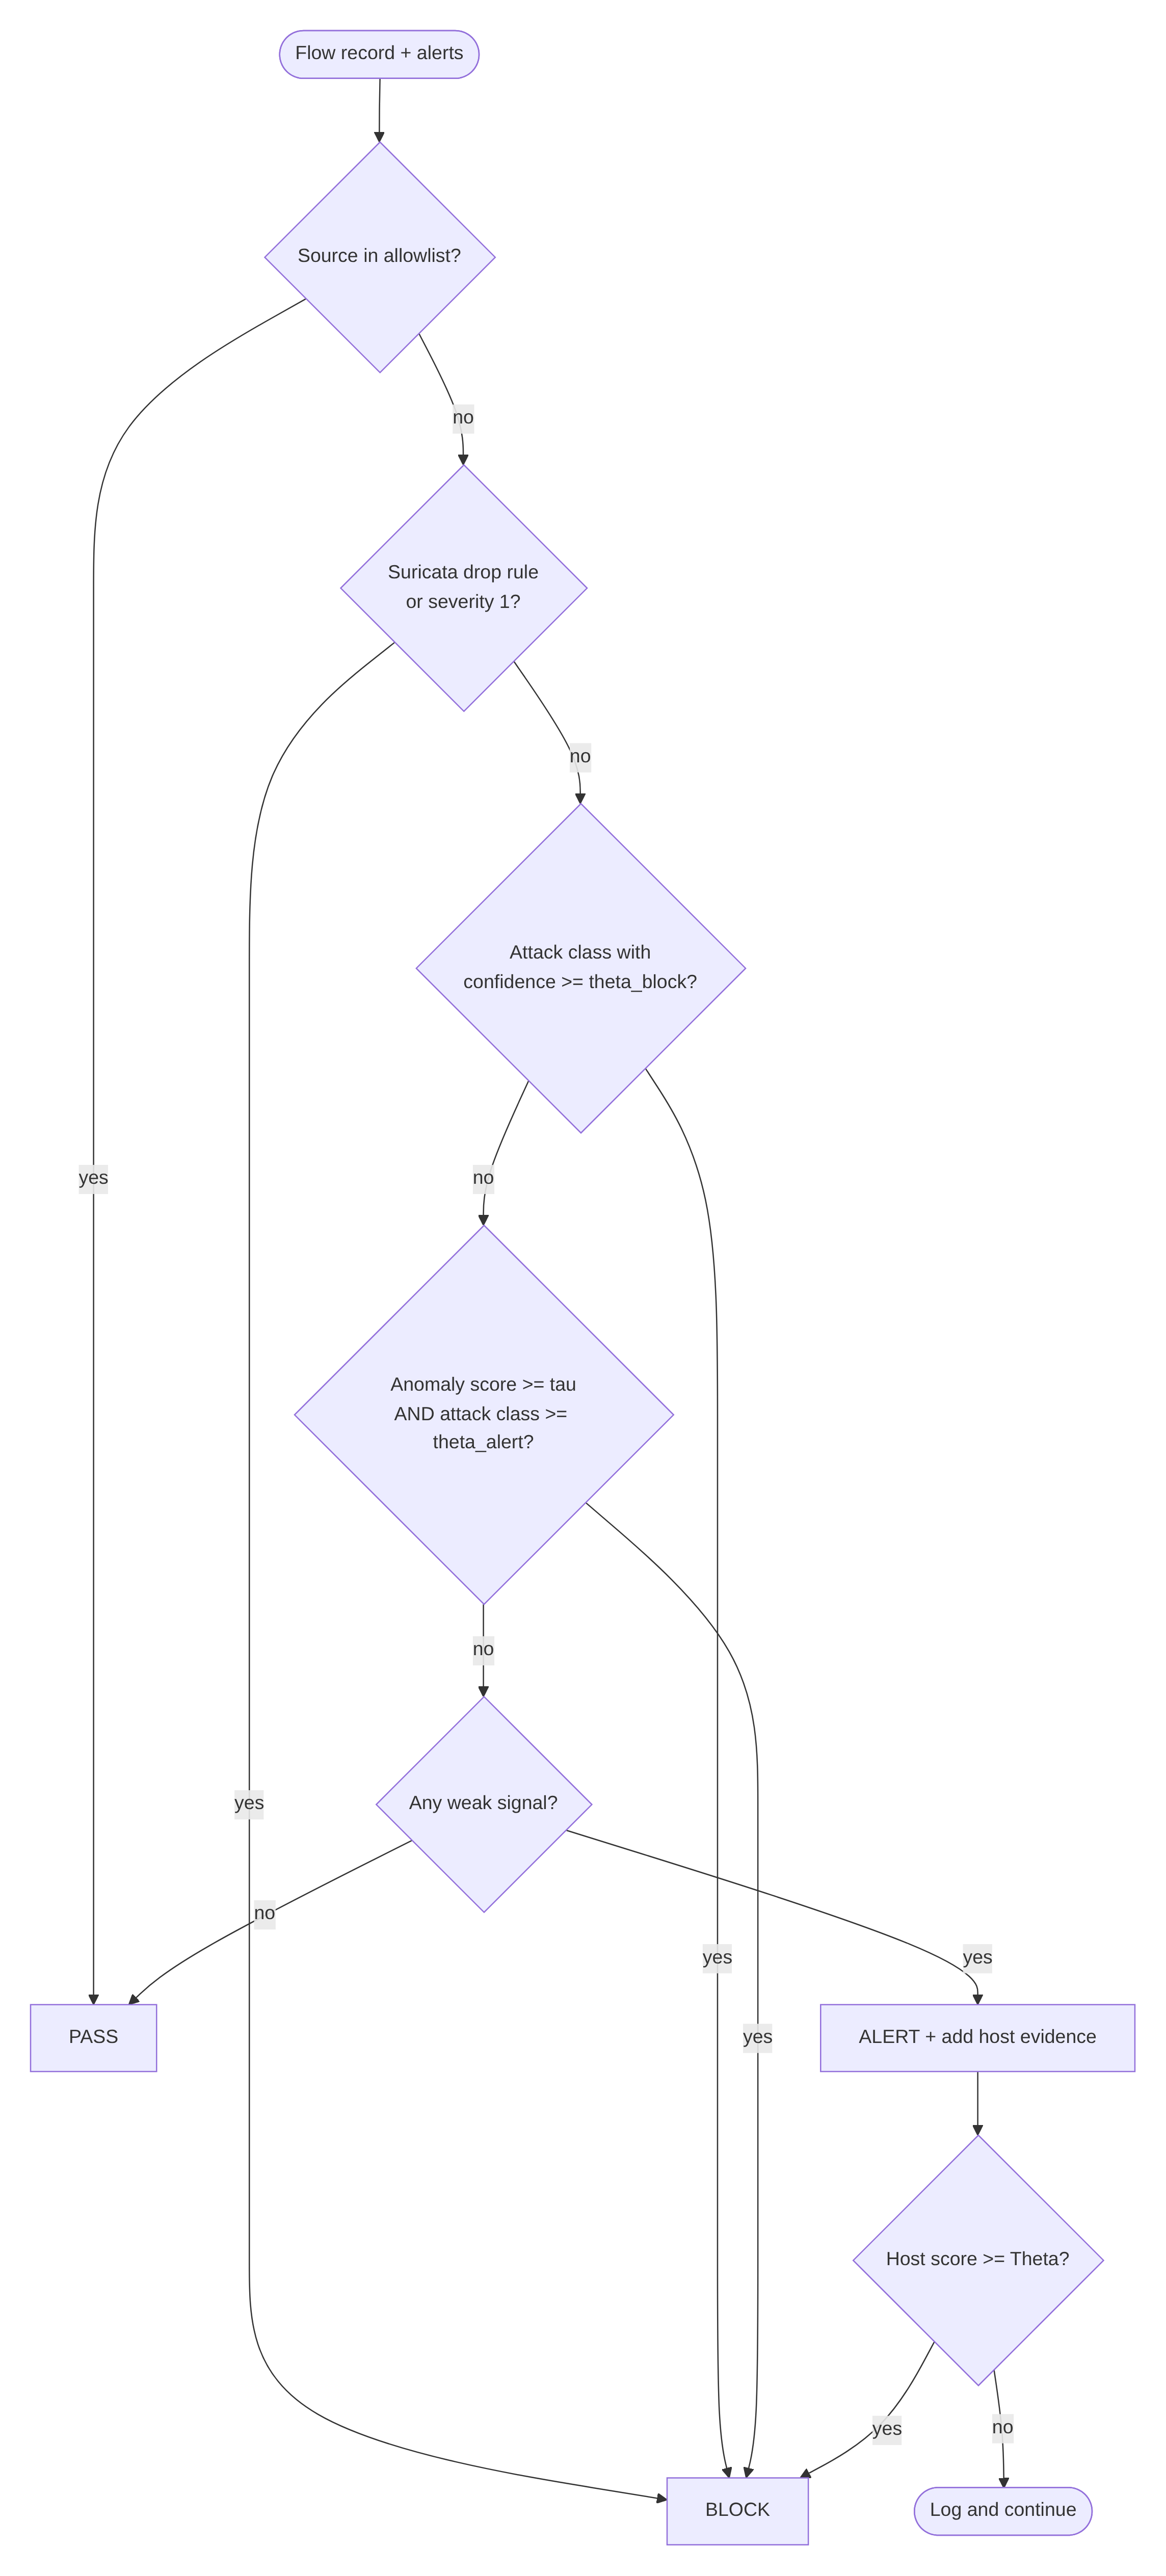
\includegraphics[width=0.62\textwidth]{Figures/nidps_fig5_2.png}
    \caption{Decision-fusion flow for one flow record.}
    \label{fig:fusion}
\end{figure}

\subsection{Host Evidence Accumulation}\label{sec:5.7.2}
\label{sec:hostscore}
\noindent Some attacks, such as a slow port scan or low-volume exfiltration, never produce one strong signal. Their individual flows only trigger alerts. The host score $S_h$ collects this weak evidence and lets it fade over time, so that a single stray alert does not lead to a block but a steady stream of alerts does:
\begin{equation}
\label{eq:hostscore}
S_h(t) = S_h(t_{prev})\, e^{-\lambda (t - t_{prev})} + w_v
\end{equation}
\noindent Here $w_v$ is the weight of the new alert (for example, higher for a Suricata alert than for an anomaly score just above $\tau$) and $\lambda$ is a decay rate. With a half-life of 10 minutes, $\lambda = \ln 2 / 600\ \mathrm{s}^{-1}$. When $S_h$ reaches the block threshold $\Theta$, the host is blocked. The same score is shown on the dashboard as the host's current risk level.

\subsection{Timing of ML Verdicts}\label{sec:5.7.3}
\label{sec:mltiming}
\noindent Layers 2 and 3 score completed flows or active-timeout segments (Algorithm~\ref{alg:flow}), so their verdict comes after part of the traffic has passed. Their blocks therefore apply to the rest of a long flow and to all later traffic from that source. This is acceptable for the attacks they target: beaconing, exfiltration, DDoS and lateral movement all unfold over many flows. Attacks that must be stopped at the first packet are the responsibility of Layer 1.

\noindent With the default $T_a = 10$\,s, the worst-case delay for an ML verdict on a long flow is about 10 seconds plus scoring time, which is milliseconds for tree models. The data that can leave over one connection before a block is therefore roughly the upload rate $\times$ that delay. This exposure is measured directly in the live exfiltration tests as ``bytes leaked before block'' (Table~\ref{tab:sysperf}), rather than estimated.

\section{Automated Prevention}\label{sec:5.8}
\label{sec:prevention}
\noindent A BLOCK verdict is turned into a firewall entry by the enforcer. The enforcer must stop attacks quickly without ever locking the owner out of their own network, so blocking follows a strict procedure.

\subsection{Blocking Mechanism}\label{sec:5.8.1}
\label{sec:blockmech}
\noindent Blocked addresses are stored in an ipset with a per-entry timeout, referenced by a single iptables rule placed before the NFQUEUE rule in the FORWARD chain (and in INPUT, to protect the AP itself). Adding or removing an address changes only the set, not the rule list, so a block takes effect immediately and costs the same regardless of how many addresses are blocked. Entries expire automatically, so a block never outlives its intended duration even if the enforcer crashes.

\subsection{Blocking Procedure}\label{sec:5.8.2}
\label{sec:blockproc}
\noindent Algorithm~\ref{alg:block} gives the procedure followed for every BLOCK verdict.

\begin{algorithm}[H]
\caption{Enforce a BLOCK verdict}
\label{alg:block}
\KwIn{offending address $a$; attack class $y$; attributed layer(s)}
\KwOut{ipset entry and audit record}
\If{$a \in$ allowlist (AP, gateway, DNS resolver, admin devices)}{
    log ``block suppressed''\; \Return{}\;
}
\If{blocks issued in the last minute $\geq R_{max}$}{
    downgrade to ALERT\; raise a ``block rate limit'' warning\; \Return{}\;
}
$n \leftarrow$ number of earlier blocks of $a$ within 24\,h\;
$duration \leftarrow \min(D_0 \cdot 2^n,\ D_{max})$ \tcp*{e.g.\ $D_0 = 5$\,min, $D_{max} = 24$\,h}
add $a$ to the ipset with timeout $duration$\;
write audit record $\{a, y, \mathrm{layers}, duration, \mathrm{evidence}, \mathrm{time}\}$\;
push the event to the dashboard\;
\end{algorithm}

\noindent The allowlist check prevents the system from cutting off its own infrastructure, even when an attacker forges packets from those addresses. The rate limit stops a flood of false positives, or an attacker spoofing many sources, from turning the NIDPS into a denial-of-service tool against its own users. Exponential back-off means a first offence is blocked briefly, in case it was a false positive, while repeat offenders are blocked for longer. Every block can be lifted manually from the dashboard.

\section{Fault Tolerance and Failure Handling}\label{sec:5.9}
\label{sec:failure}
\noindent An inline security device is itself a single point of failure: if Suricata crashes while traffic is queued to it, the whole network can go down. The NIDPS therefore defines exactly what happens when each component fails, and lets the owner choose between availability and security.

\subsection{Health Monitoring}\label{sec:5.9.1}
\label{sec:health}
\noindent Every component (Suricata, flow assembler, ML scorer, decision engine, enforcer) runs as a separate systemd service. Each one sends a heartbeat to the watchdog every second, along with load indicators such as queue depth and processing lag. A component is declared failed after $k = 3$ missed heartbeats or if its process exits. systemd restarts failed services automatically, and its own watchdog timer restarts services that are running but frozen.

\subsection{Failure Modes}\label{sec:5.9.2}
\label{sec:failuremodes}
\noindent Table~\ref{tab:failuremodes} lists the configurable failure modes.

\begin{table}[H]
\centering
\caption{Configurable failure modes.}
\label{tab:failuremodes}
\begin{tabular}{|>{\raggedright\arraybackslash}p{0.15\linewidth}|>{\raggedright\arraybackslash}p{0.24\linewidth}|>{\raggedright\arraybackslash}p{0.28\linewidth}|>{\raggedright\arraybackslash}p{0.18\linewidth}|}
\hline
\textbf{Mode} & \textbf{When Layer 1 fails} & \textbf{When an ML layer fails} & \textbf{Suited to} \\
\hline
Fail-open & Packets bypass the queue and are forwarded uninspected & Remaining layers continue; affected flows are logged as unscored & Homes where internet access matters most \\
\hline
Fail-closed & Forwarded traffic is dropped until recovery; admin access to the AP stays open & Flows from unknown hosts are held at ALERT and new block decisions rely on Layer 1 only & Small offices handling sensitive data \\
\hline
Degraded (load-shedding) & Non-essential rule groups are disabled to reduce load & Only a sample of flows (1 in $k$) is scored, prioritising new and high-risk hosts & Temporary overload rather than a crash \\
\hline
\end{tabular}
\end{table}

\noindent Fail-open is implemented in the kernel rather than in software: the NFQUEUE rule is created with the queue-bypass option, so when no process is attached to the queue, the kernel accepts packets instead of dropping them. Fail-closed omits this option. Because the kernel enforces the mode, it holds even when the watchdog itself has crashed.

\subsection{State Machine}\label{sec:5.9.3}
\label{sec:statemachine}
\noindent Figure~\ref{fig:statemachine} shows the states each supervised component moves through.

\begin{figure}[!htbp]
    \centering
    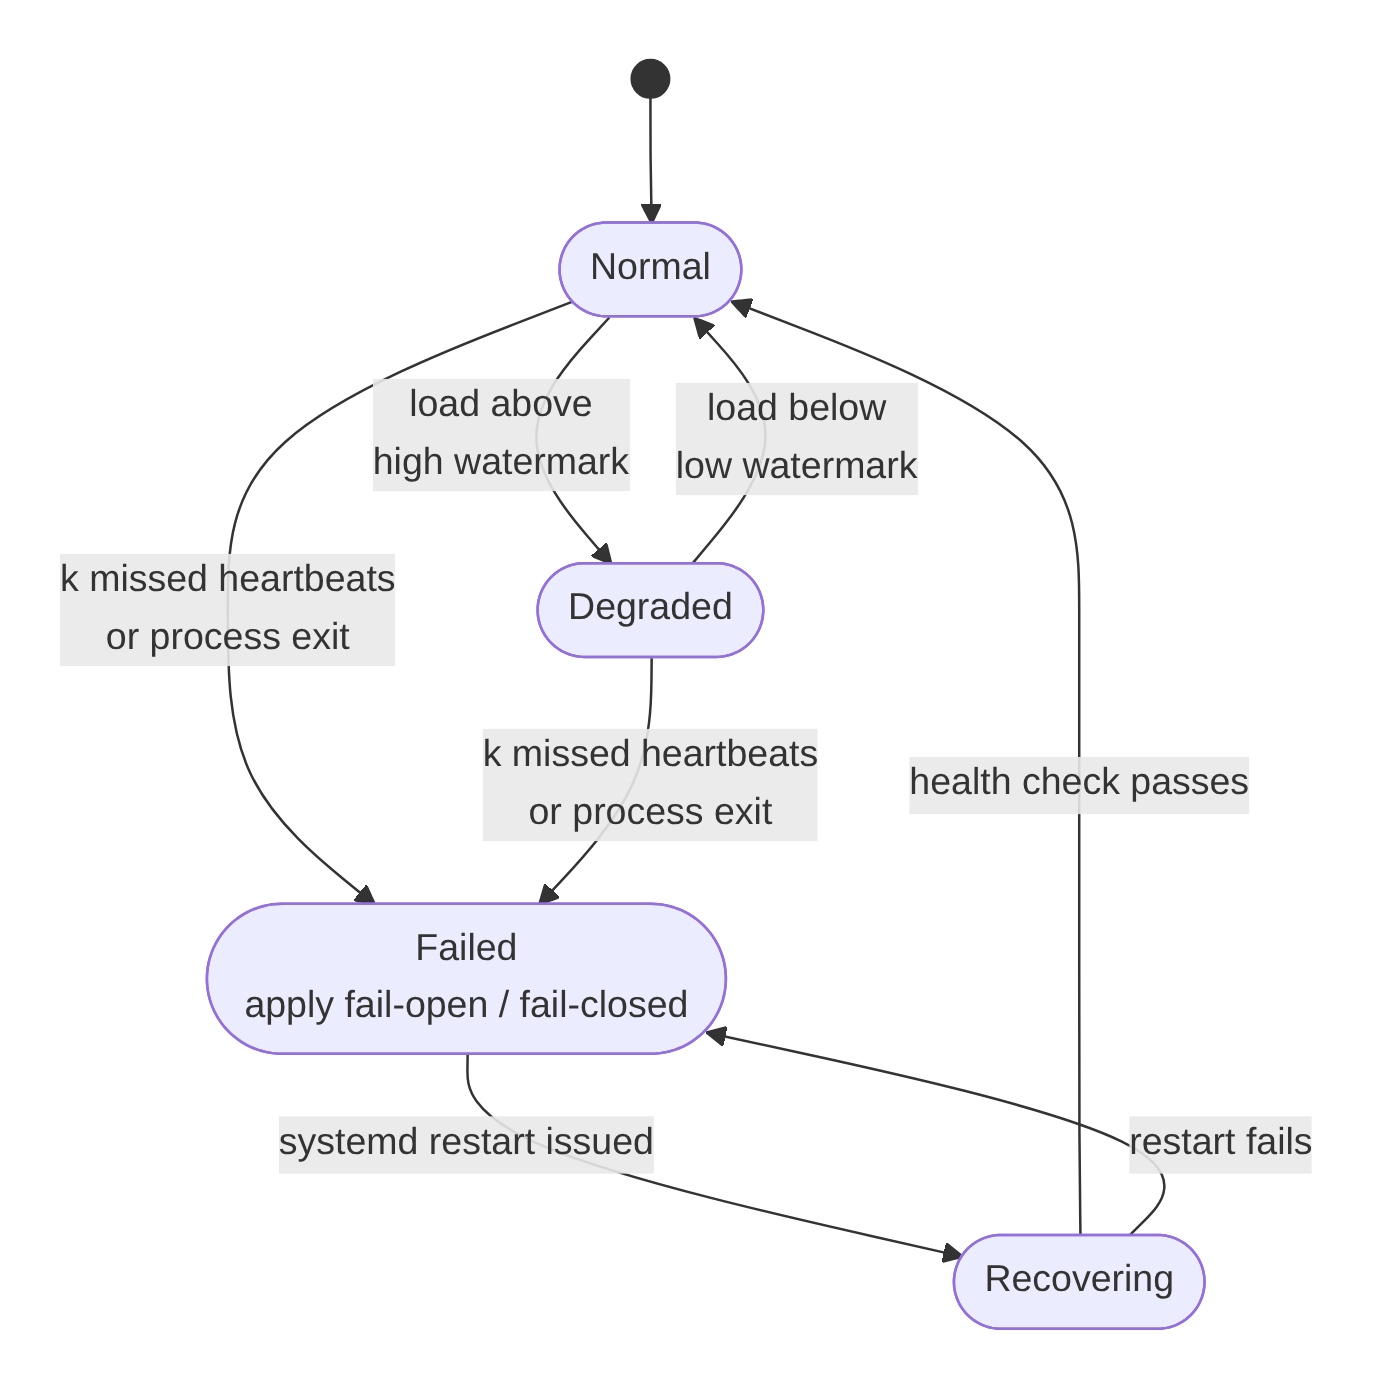
\includegraphics[width=0.55\textwidth]{Figures/nidps_fig5_3.png}
    \caption{Watchdog state machine for each supervised component.}
    \label{fig:statemachine}
\end{figure}

\noindent Two thresholds (high and low watermarks) are used for entering and leaving the degraded state. Without this gap, a load hovering around one value would cause the system to switch modes back and forth many times per second. During every failure, the watchdog records when it was detected, which mode was applied, when service resumed and how many packets were dropped or bypassed. These records produce the recovery measurements reported in the evaluation.

\section{Evaluation Methodology}\label{sec:5.10}
\label{sec:evaluation}
\noindent The system is evaluated on two questions: how well it detects attacks, and whether it can do so inline on constrained hardware without harming the network.

\subsection{Detection Metrics}\label{sec:5.10.1}
\label{sec:metrics}
\noindent For every layer and for the fused system, precision, recall, F1-score and false positive rate (FPR) are reported per class and macro-averaged:
\begin{equation}
\label{eq:metrics}
\begin{aligned}
\mathrm{Precision} &= \frac{TP}{TP + FP}, \qquad &
\mathrm{Recall} &= \frac{TP}{TP + FN}, \\
F_1 &= \frac{2 \cdot \mathrm{Precision} \cdot \mathrm{Recall}}{\mathrm{Precision} + \mathrm{Recall}}, \qquad &
\mathrm{FPR} &= \frac{FP}{FP + TN}
\end{aligned}
\end{equation}
\noindent False positive rate receives particular attention. On a home network producing thousands of flows per hour, even a 1\% false positive rate means dozens of wrong alerts or blocks every hour. For Layer 2, the area under the precision-recall curve is also reported, since it summarises performance across all thresholds and is more informative than ROC-AUC when attacks are rare.

\subsection{Cross-Dataset Generalisation}\label{sec:5.10.2}
\label{sec:crossdataset}
\noindent Each model is trained on one dataset and tested on every other dataset, giving the matrix in Table~\ref{tab:crossmatrix}. The diagonal (train and test on the same dataset, split by day) shows in-distribution performance. The off-diagonal cells show how much performance drops when the network changes, which is the realistic situation for a deployed device. Finally, models trained on all three public datasets combined are tested on the self-collected dataset.

\begin{table}[H]
\centering
\caption{Cross-dataset evaluation matrix of macro F1-scores, to be filled from experiments.}
\label{tab:crossmatrix}
\begin{tabular}{|>{\raggedright\arraybackslash}p{0.22\linewidth}|>{\raggedright\arraybackslash}p{0.14\linewidth}|>{\raggedright\arraybackslash}p{0.16\linewidth}|>{\raggedright\arraybackslash}p{0.14\linewidth}|>{\raggedright\arraybackslash}p{0.14\linewidth}|}
\hline
\textbf{Train / Test} & \textbf{CIC-IDS-2017} & \textbf{CSE-CIC-IDS2018} & \textbf{CIC-IoT-2023} & \textbf{Self-collected} \\
\hline
CIC-IDS-2017 & in-distribution & & & \\
\hline
CSE-CIC-IDS2018 & & in-distribution & & \\
\hline
CIC-IoT-2023 & & & in-distribution & \\
\hline
All three combined & & & & \\
\hline
\end{tabular}
\end{table}

\noindent Only classes that exist in both the training and the test dataset are scored in each cell. The adaptive threshold of Section~\ref{sec:calibration} is evaluated by comparing the false positive rate on the self-collected benign traffic with the global threshold and with the calibrated threshold.

\subsection{System Performance on Constrained Hardware}\label{sec:5.10.3}
\label{sec:sysperf}
\noindent Table~\ref{tab:sysperf} defines the system-level measures and how each is obtained.

\begin{table}[H]
\centering
\caption{System performance measures.}
\label{tab:sysperf}
\begin{tabular}{|>{\raggedright\arraybackslash}p{0.2\linewidth}|>{\raggedright\arraybackslash}p{0.3\linewidth}|>{\raggedright\arraybackslash}p{0.38\linewidth}|}
\hline
\textbf{Measure} & \textbf{Definition} & \textbf{How it is measured} \\
\hline
Forwarding latency & Extra round-trip time added by the NIDPS & Ping RTT through the AP with the NIDPS off, then with each layer enabled in turn \\
\hline
Throughput & Sustained forwarding rate & iperf3 TCP and UDP tests through the AP, layers enabled incrementally \\
\hline
Detection latency & Time from the first attack packet to the alert & Attack start logged on the attacker machine vs.\ alert timestamp \\
\hline
Time to block & Time from the first attack packet to the ipset entry & Same, against the audit record \\
\hline
Bytes leaked before block & Data the attacker transferred before the block took effect & Bytes received at the lab exfiltration server before the block, repeated at $T_a = 5$\,s and 10\,s \\
\hline
Resource use & CPU, memory and temperature of the host & Sampled every second during each test, at $T_a = 5$\,s and 10\,s \\
\hline
Recovery behaviour & Time to detect a failure, time to restore service, packets lost or bypassed & Components killed deliberately under load, in each failure mode \\
\hline
\end{tabular}
\end{table}

\noindent Every attack in the scope is replayed live against test devices on the isolated lab network while background benign traffic runs. This end-to-end test checks the complete chain, from detection through fusion to blocking, rather than each model in isolation.

\section{Conclusion}\label{sec:5.11}
\label{sec:ch5conclusion}
\noindent This chapter presented the proposed hybrid framework and the backend algorithms behind it. Suricata and an ARP consistency check provide fast, packet-level detection of known attacks. Isolation Forest, with a per-network threshold calibration, detects unusual behaviour, supported by host-level scores for exfiltration and C2 beaconing. A Random Forest or XGBoost classifier assigns flows to known attack families. Encrypted traffic is analysed through JA3/JA3S fingerprints and flow statistics instead of decryption, and all datasets are regenerated with the device's own flow extractor so training and runtime features match. A decision-fusion algorithm with host evidence accumulation turns these signals into verdicts, an enforcer applies them through timed ipset entries with safeguards against self-inflicted outages, and a watchdog applies a configurable failure mode backed by the kernel. The evaluation protocol measures both detection quality across datasets and the system's latency, throughput and recovery on real hardware. The next chapter describes how these algorithms are organised into components and how those components interact.

\chapter{High-Level and Low-Level Design}\label{chap:6}
\label{chap:design}
\noindent This chapter describes how the methodology of Chapter~\ref{chap:approach} is realised as software. It moves from the high level to the low level: first an overview of the system and the considerations that shaped its design, then the architecture of the whole system and of each subsystem, the strategies behind the main architectural decisions, the class diagram, and finally the policies and tactics that govern implementation, testing and maintenance.

\section{System Overview}\label{sec:6.1}
\label{sec:sysoverview}
\noindent The NIDPS is a self-contained security appliance built from software on a single Linux host. The host replaces the role of the home router's wireless network: clients connect to the NIDPS access point, and the NIDPS routes their traffic, through its own NAT, to the existing ISP router, which keeps handling the internet connection. No change is needed on client devices or on the ISP router.

\noindent Functionally, the system does five things:
\begin{enumerate}
    \item \textbf{Provides network access:} a wireless access point with DHCP, DNS and routing.
    \item \textbf{Inspects traffic:} inline signature inspection of every packet, plus flow-level analysis of all traffic, including encrypted traffic through metadata.
    \item \textbf{Decides:} fuses signature, anomaly and classification results into a per-flow verdict and a per-host risk score.
    \item \textbf{Responds:} blocks offending addresses automatically for a limited, escalating time.
    \item \textbf{Reports and stays available:} shows live statistics and alerts on a web dashboard, and keeps the network in a defined state when a component fails.
\end{enumerate}

\noindent The system is made up of independent services connected by a local event bus, rather than as one large program. The packet-forwarding path is kept as short as possible (kernel plus Suricata), and everything slower like machine learning, the database and the dashboard, sits beside that path instead of in it. Sections~\ref{sec:sysarch} and~\ref{sec:archstrategies} explain this choice in detail.

\section{Design Considerations}\label{sec:6.2}
\label{sec:designconsiderations}
\noindent This section records the assumptions, constraints, goals and development methods that shaped the design.

\subsection{Assumptions and Dependencies}\label{sec:6.2.1}
\label{sec:assumptions}
\begin{itemize}
    \item \textbf{Hardware:} the host is a mid-range laptop or a Raspberry Pi with at least 4\,GB of RAM, a wireless adapter that supports AP mode and an Ethernet port for the uplink.
    \item \textbf{Operating system:} Debian based Linux distribution with systemd, iptables (use of nftables is accepted, but not required), ipset (use of NFQUEUE is accepted, but not required) and support in the kernel.
    \item \textbf{Network position:} NIDPS is the only wireless network clients access. Devices which are connected directly to the ISP router via cable or directly by the ISP router's Wi-Fi are not protected. Turning off the ISP router's WiFi is a part of the set-up process.
    \item \textbf{Third-party software:} Suricata 7 or later with Emerging Threats Open ruleset, hostapd, dnsmasq, Python 3.11+ with scikit-learn and XGBoost. Periodic Internet access is required for ruleset updates.
    \item \textbf{End users:} Owner is NOT a security expert. Defaults should be safe and not require tuning, and dashboard should provide information about alerts in easy-to-understand terms.
    \item \textbf{Trust:} The NIDPS host and the admin's devices are trusted. The ISP router is assumed to be working, but is not trusted to provide any security.
    \item \textbf{Likely changes:} Changes are likely to include new attack types and new rules, models may be retrained and the TLS fingerprinting method could change from JA3 to its successor JA4, as TLS client libraries start to shuffle the order of extensions. Each of these is isolated by the design behind its component.
\end{itemize}

\subsection{General Constraints}\label{sec:6.2.2}
\label{sec:constraints}
\noindent Table~\ref{tab:constraints} lists the global constraints and their impact on the design.

\begin{table}[H]
\centering
\caption{General constraints and their impact on the design.}
\label{tab:constraints}
\begin{tabular}{|>{\raggedright\arraybackslash}p{0.18\linewidth}|>{\raggedright\arraybackslash}p{0.2\linewidth}|>{\raggedright\arraybackslash}p{0.5\linewidth}|}
\hline
\textbf{Constraint} & \textbf{Source} & \textbf{Impact on the design} \\
\hline
Limited CPU and memory & Low-cost target hardware & Tree-based models instead of deep networks; per-flow rather than per-packet ML; incremental feature statistics; rule groups trimmed to the home-network scope \\
\hline
Inline position & The NIDPS forwards all traffic & Forwarding path kept to kernel + Suricata; ML runs off-path; failure mode enforced in the kernel \\
\hline
Encrypted traffic & Most traffic uses TLS/QUIC & No payload inspection for ML; detection from flow metadata and JA3/JA3S only \\
\hline
Privacy & Household traffic is personal & No decryption; no payload storage; only flow metadata and alerts are kept, with a retention limit \\
\hline
Availability & A home network must not go down & Configurable fail-open default; block rate limits; allowlist; ipset entries that expire \\
\hline
Interoperability & Training data and live traffic must match & One flow extractor used offline and online; model files carry their feature schema \\
\hline
Security of the device & The NIDPS is itself a target & Dashboard bound to the LAN only, authenticated, management traffic allowlisted; services run without root where possible \\
\hline
Testability & Attacks cannot be run on real users & Isolated lab network and attacker machine for all attack tests \\
\hline
\end{tabular}
\end{table}

\subsection{Goals and Guidelines}\label{sec:6.2.3}
\label{sec:goals}
\begin{enumerate}
    \item \textbf{Never make the network worse than a plain router.} Every design choice is checked against this. It is why fail-open is the default, why blocks expire and why the number of blocks per minute is capped.
    \item \textbf{Keep the fast path short (KISS).} Only the kernel and Suricata sit in the forwarding path. Anything that can be done after the fact is moved off it.
    \item \textbf{Defence in depth.} No single detector is trusted to catch everything; each layer covers a weakness of the others (Section~\ref{sec:overview}).
    \item \textbf{Speed over memory where the two conflict, within a fixed budget.} Models and rule sets are loaded fully in memory to avoid disk access during inspection, but their size is capped to fit the hardware.
    \item \textbf{Explainable decisions.} Every block records which layer decided, why, and with what evidence, so the owner can trust or override it.
    \item \textbf{Same code for training and serving.} Features are computed by one implementation to rule out train/serve skew.
    \item \textbf{Configurable, safe defaults.} Thresholds, failure mode and block durations are configurable, but the defaults work without tuning.
\end{enumerate}

\subsection{Development Methods}\label{sec:6.2.4}
\label{sec:devmethods}
\noindent The project follows an iterative, incremental approach in short sprints of two weeks, aligned with the FYP milestones. Each increment delivers a working vertical slice: first the access point with Suricata (Layer 1, completed), then flow extraction and Layer 2, then Layer 3, then fusion and enforcement, and finally the watchdog and dashboard. This order means the system protects the network from the first increment onwards and every later layer can be measured against a working baseline.

\noindent The machine learning work follows the CRISP-DM cycle (data understanding, preparation, modelling, evaluation, deployment), because model quality depends on several rounds of data cleaning and re-evaluation. A plain waterfall model was considered and rejected: detection performance on real traffic cannot be known in advance, so requirements such as thresholds and feature sets must be allowed to change as results come in.

\section{System Architecture}\label{sec:6.3}
\label{sec:sysarch}
\noindent The system is decomposed into five runtime subsystems on the NIDPS host and one offline subsystem used for training. Figure~\ref{fig:architecture} shows the external architecture (how the NIDPS sits between clients, the ISP router and the administrator) together with the internal subsystems and their main data flows.

\begin{figure}[!htbp]
    \centering
    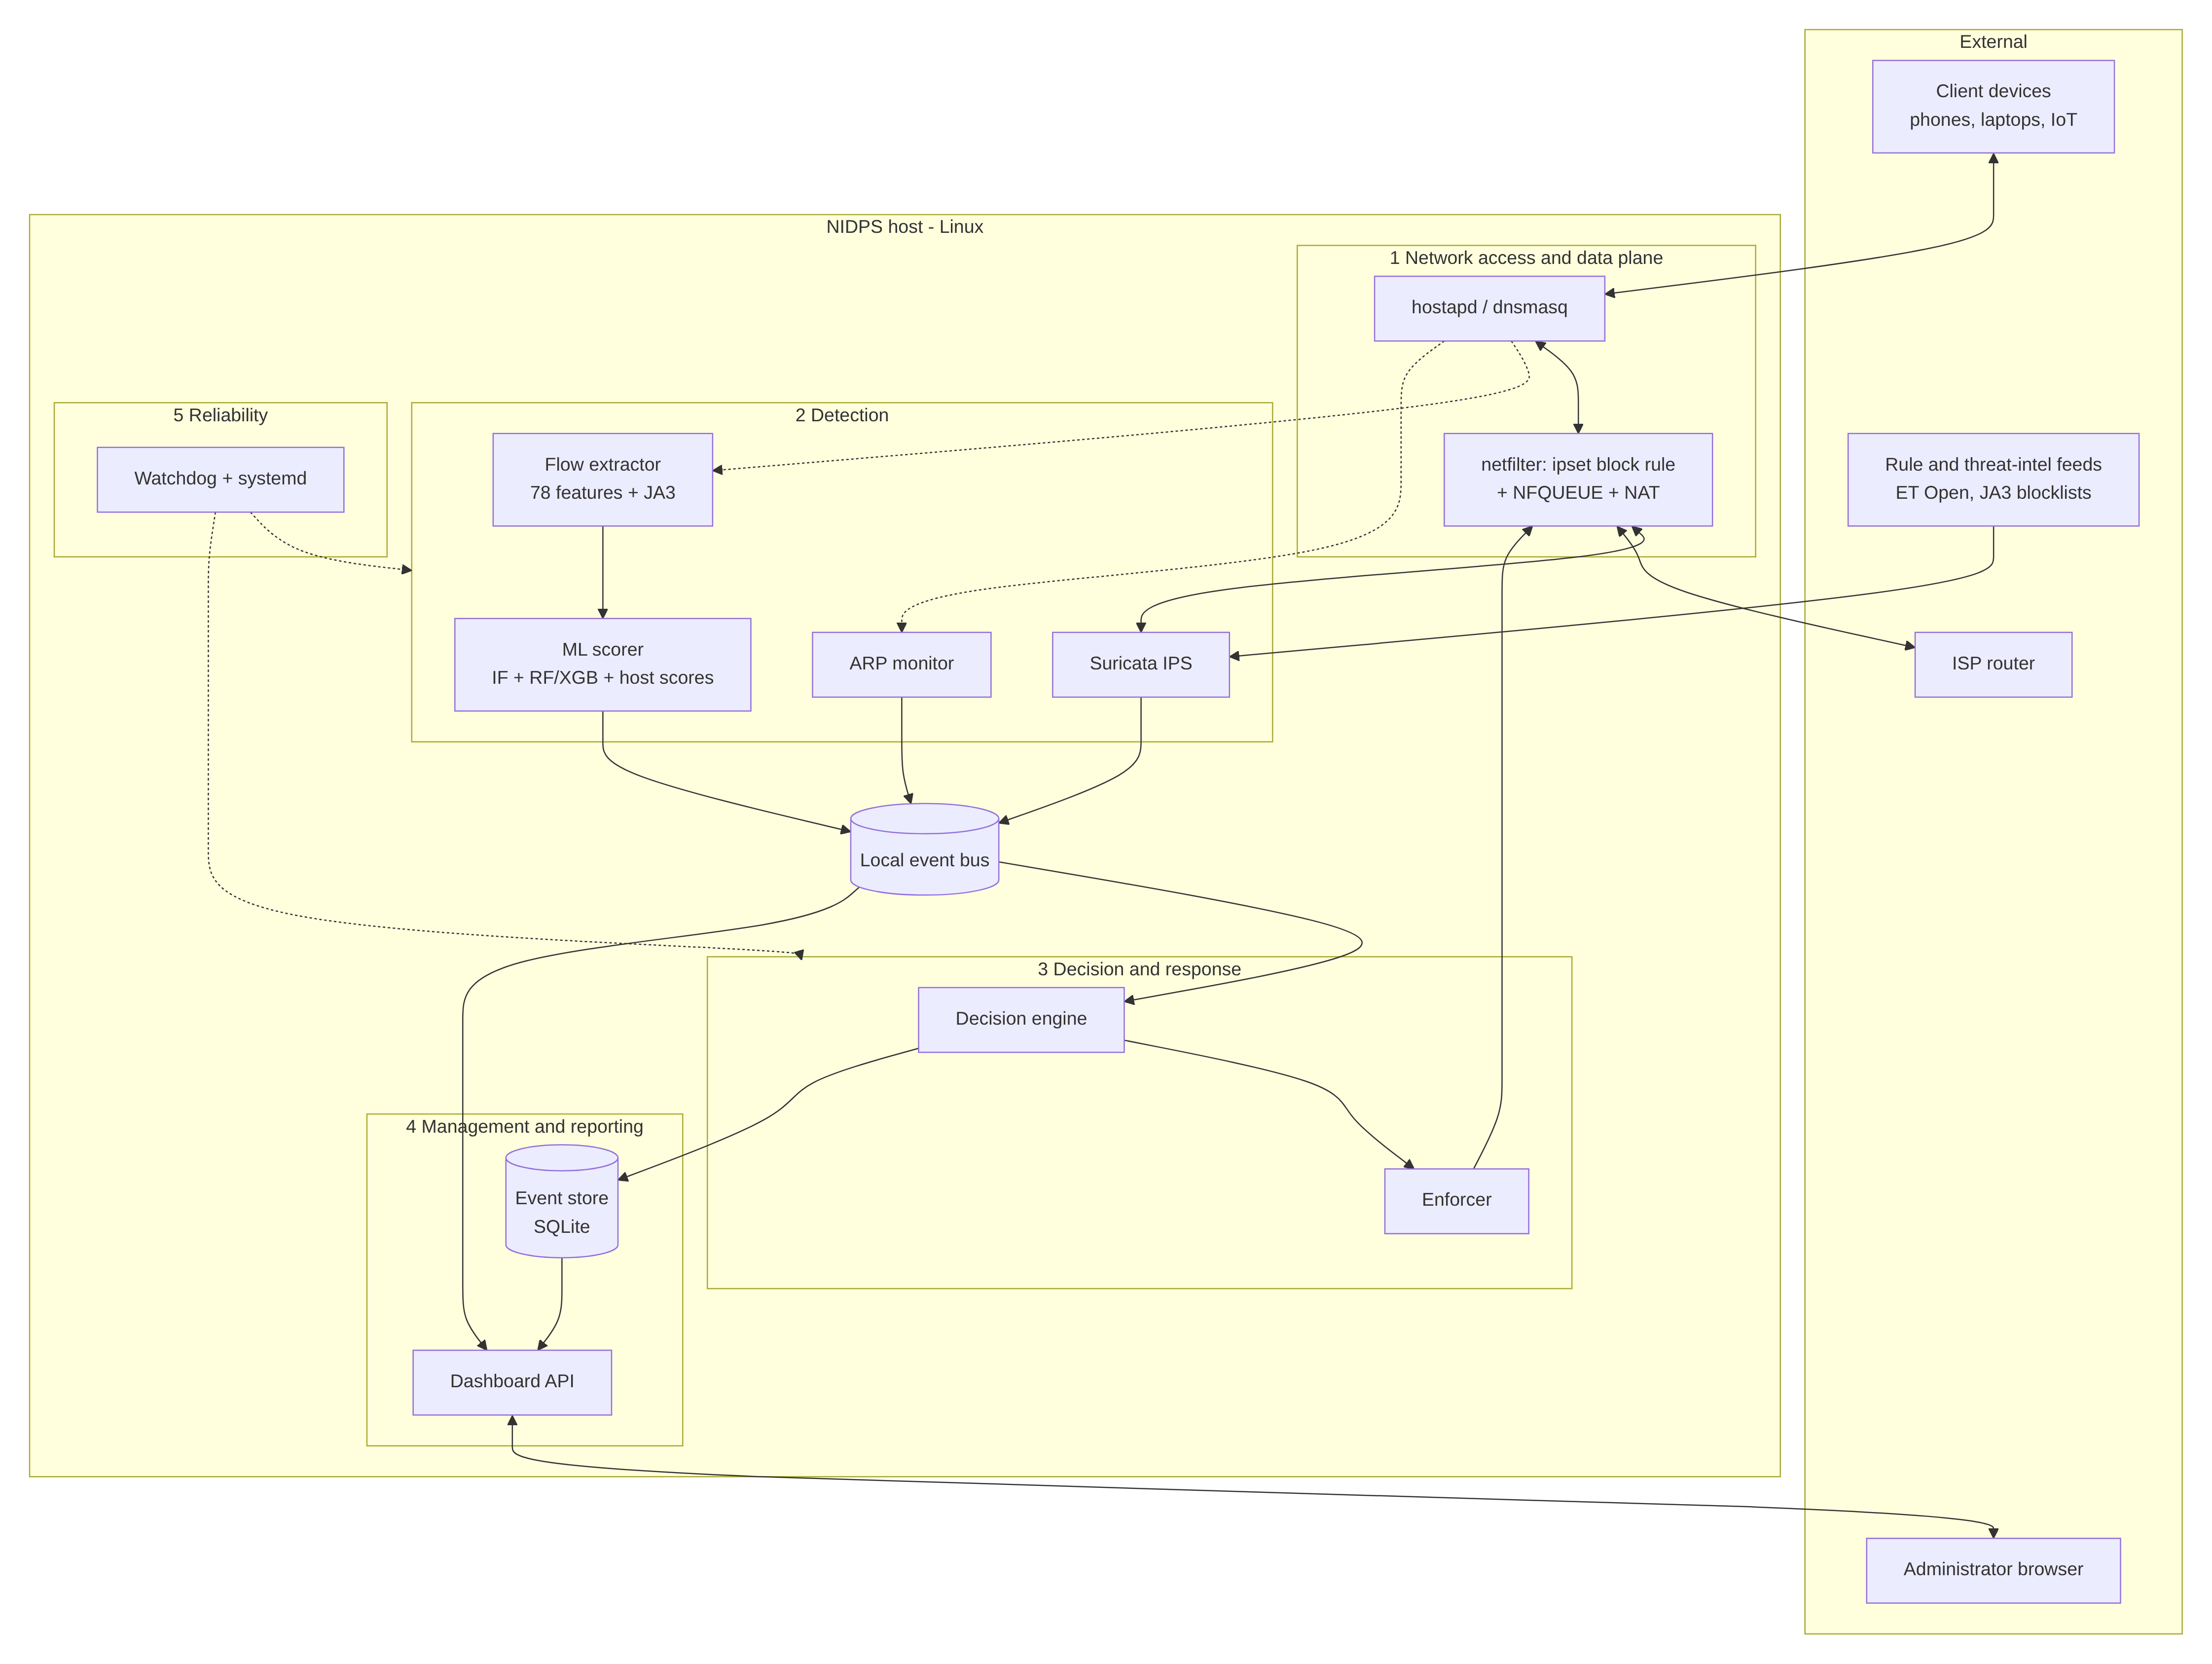
\includegraphics[width=\textwidth]{Figures/nidps_fig6_1.png}
    \caption{System architecture of the NIDPS.}
    \label{fig:architecture}
\end{figure}

\noindent The responsibilities are partitioned as shown in Table~\ref{tab:subsystems}.

\begin{table}[H]
\centering
\caption{Subsystem responsibilities.}
\label{tab:subsystems}
\begin{tabular}{|>{\raggedright\arraybackslash}p{0.22\linewidth}|>{\raggedright\arraybackslash}p{0.38\linewidth}|>{\raggedright\arraybackslash}p{0.28\linewidth}|}
\hline
\textbf{Subsystem} & \textbf{Responsibility} & \textbf{Main components} \\
\hline
1. Network access and data plane & Provide Wi-Fi, addressing and routing; hold the inline queue; enforce blocks and failure mode in the kernel & hostapd, dnsmasq, netfilter (iptables, ipset, NFQUEUE, NAT) \\
\hline
2. Detection & Produce evidence: signature alerts, ARP alerts, flow records, anomaly scores, class probabilities & Suricata, ARP monitor, flow extractor, ML scorer \\
\hline
3. Decision and response & Turn evidence into verdicts and host risk; apply and expire blocks & Decision engine, enforcer \\
\hline
4. Management and reporting & Store events; expose live statistics, alerts and configuration to the admin & Event store, dashboard API and web UI, configuration manager \\
\hline
5. Reliability & Detect failed or overloaded components; restart them; apply failure mode; record recovery metrics & Watchdog, systemd units \\
\hline
Offline: training & Regenerate datasets, train and validate models, publish versioned model files & Dataset builder, trainer, model registry \\
\hline
\end{tabular}
\end{table}

\noindent The subsystems collaborate through two channels. The forwarding path is purely in the kernel and Suricata, with a single feedback loop from the enforcer into ipset. All other communication goes through the local event bus: detectors publish evidence, the decision engine consumes it and publishes verdicts, and the dashboard and event store subscribe to everything. Detectors therefore never call the decision engine directly, and a slow or crashed consumer never blocks a producer.

\noindent \textbf{Rationale and rejected alternatives.} Three decompositions were considered. A \emph{single monolithic process} would be simplest to write, but one crash in the ML code would take down detection entirely, and memory would be shared by everything. A \emph{distributed design} with a separate analysis server would allow larger models, but adds a second machine, network latency and cost, against the project's aim of one affordable box. The chosen \emph{local service-oriented design} keeps everything on one host while isolating failures per service, which is what the failure-handling requirement needs.

\subsection{Subsystem Architecture}\label{sec:6.3.1}
\label{sec:subsysarch}
\noindent This section describes each subsystem in more detail.

\subsubsection{Network Access and Data Plane}\label{sec:6.3.1.1}
\noindent This subsystem is mostly configuration of existing Linux components; the new parts are the netfilter rule layout and its management. Figure~\ref{fig:packetpath} traces one packet from a client to the internet.

\begin{figure}[!htbp]
    \centering
    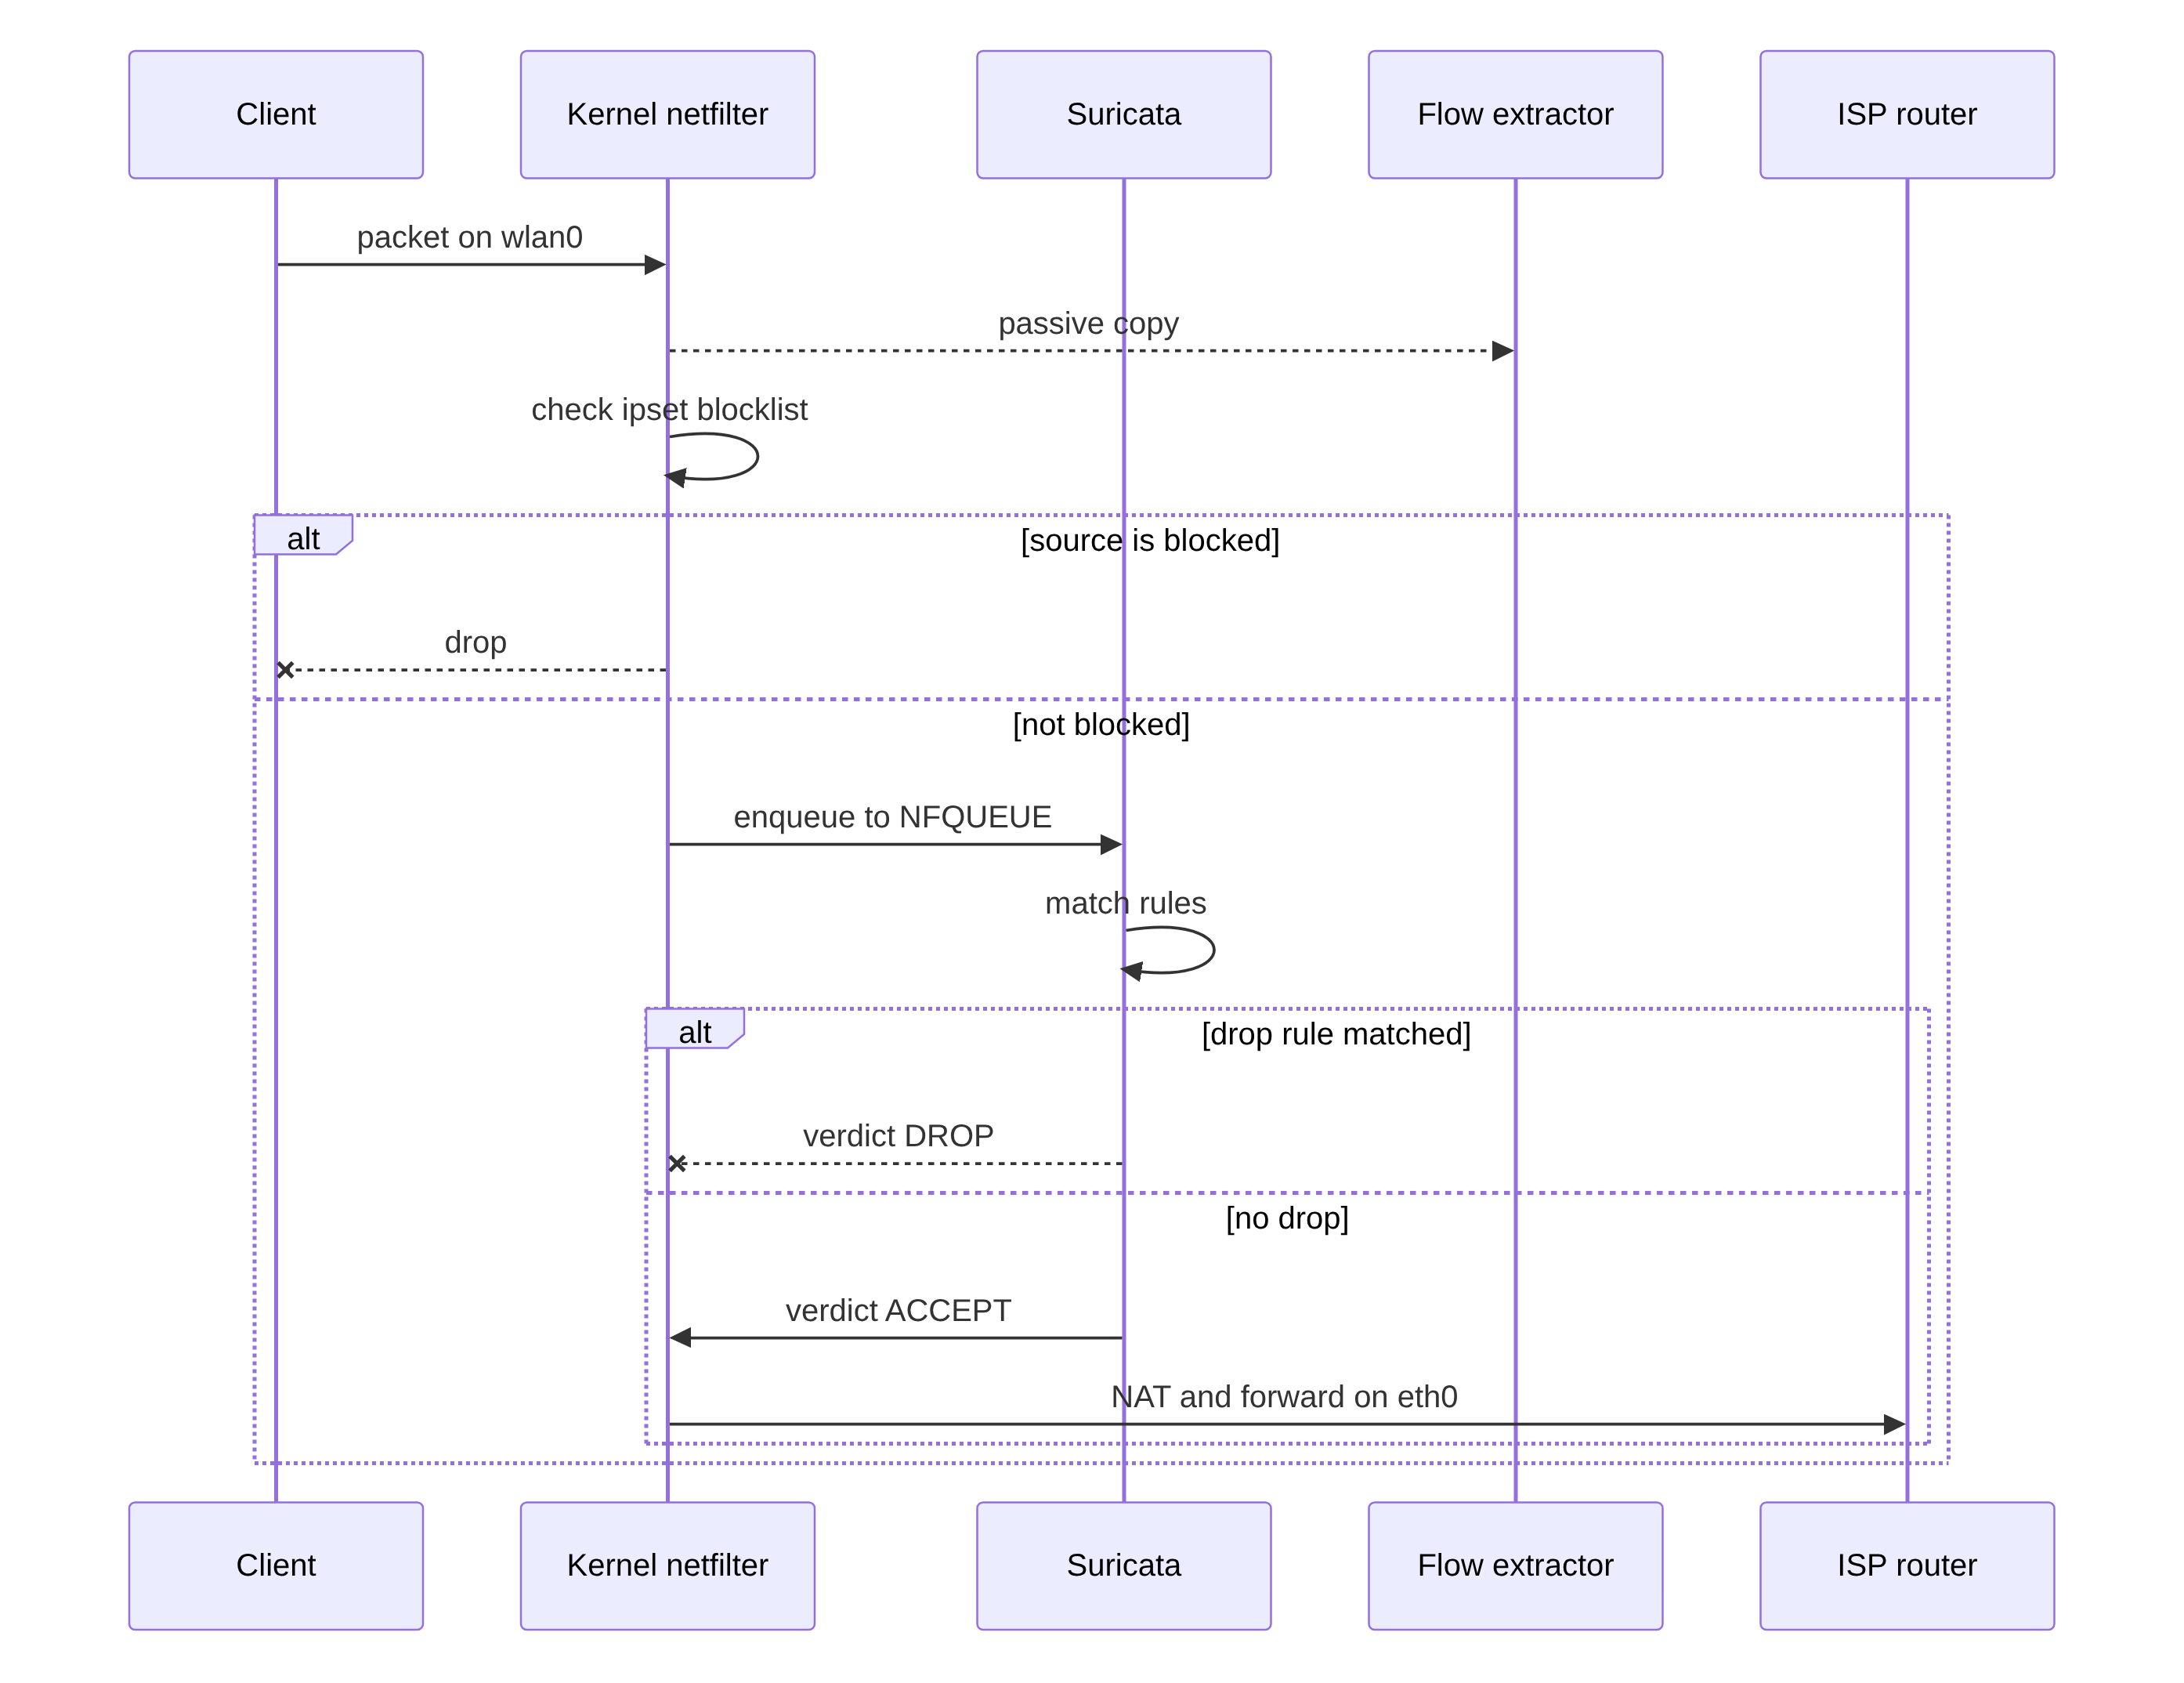
\includegraphics[width=0.85\textwidth]{Figures/nidps_fig6_2.png}
    \caption{Packet path through the data plane.}
    \label{fig:packetpath}
\end{figure}

\noindent The rule order matters: the ipset check comes before the queue, so packets from blocked hosts are discarded in the kernel and never cost Suricata any CPU. During a DDoS from a blocked source, this keeps the inspection engine free for other traffic.

\subsubsection{Detection Subsystem}\label{sec:6.3.1.2}
\noindent The detection subsystem has four producers. Suricata and the ARP monitor emit alerts directly. The flow extractor emits flow records, which the ML scorer enriches before publishing. Internally, the ML scorer is divided into three subcomponents:
\begin{itemize}
    \item \textbf{Feature validator:} checks each flow record against the model's feature schema and rejects mismatched or malformed records.
    \item \textbf{Flow models:} the Isolation Forest and the RF/XGBoost classifier, both loaded once at start-up and applied to every flow record.
    \item \textbf{Host behaviour tracker:} keeps per-host state (outbound byte baselines, per-key connection timestamps, local JA3 counts) and computes the exfiltration and beaconing scores of Sections~\ref{sec:exfil} and~\ref{sec:beacon}. Its state is bounded: entries for inactive hosts and keys expire.
\end{itemize}

\subsubsection{Decision and Response Subsystem}\label{sec:6.3.1.3}
\noindent The decision engine consumes all evidence from the bus, joins Suricata alerts with flow records by flow identifier and time, runs Algorithm~\ref{alg:verdict} and maintains the host scores of Section~\ref{sec:hostscore}. The enforcer receives BLOCK verdicts and runs Algorithm~\ref{alg:block}. The two are kept separate so that the component allowed to change firewall state is small, simple and easy to audit.

\subsubsection{Reliability Subsystem}\label{sec:6.3.1.4}
\noindent The watchdog receives heartbeats from every service and runs the state machine of Figure~\ref{fig:statemachine} for each. systemd provides process-level supervision (automatic restart, start order, resource limits), while the watchdog adds application-level health (queue depth, processing lag) and decides when to enter degraded mode. The kernel-level failure mode (queue bypass on or off) is set when the data plane starts, so it does not depend on the watchdog being alive.

\subsubsection{Management and Reporting Subsystem}\label{sec:6.3.1.5}
\noindent The dashboard API serves a web interface on the LAN side only. It provides live counters (flows per second, alerts and blocks per layer), an alert list with the evidence behind each verdict, the list of currently blocked hosts with a manual unblock action, host risk scores, component health, and configuration of thresholds, failure mode and allowlist. Configuration changes are validated, saved and published on the bus so running services pick them up without a restart.

\subsubsection{Offline Training Pipeline}\label{sec:6.3.1.6}
\noindent Figure~\ref{fig:training} shows the offline pipeline and the hand-over of models to the device.

\begin{figure}[!htbp]
    \centering
    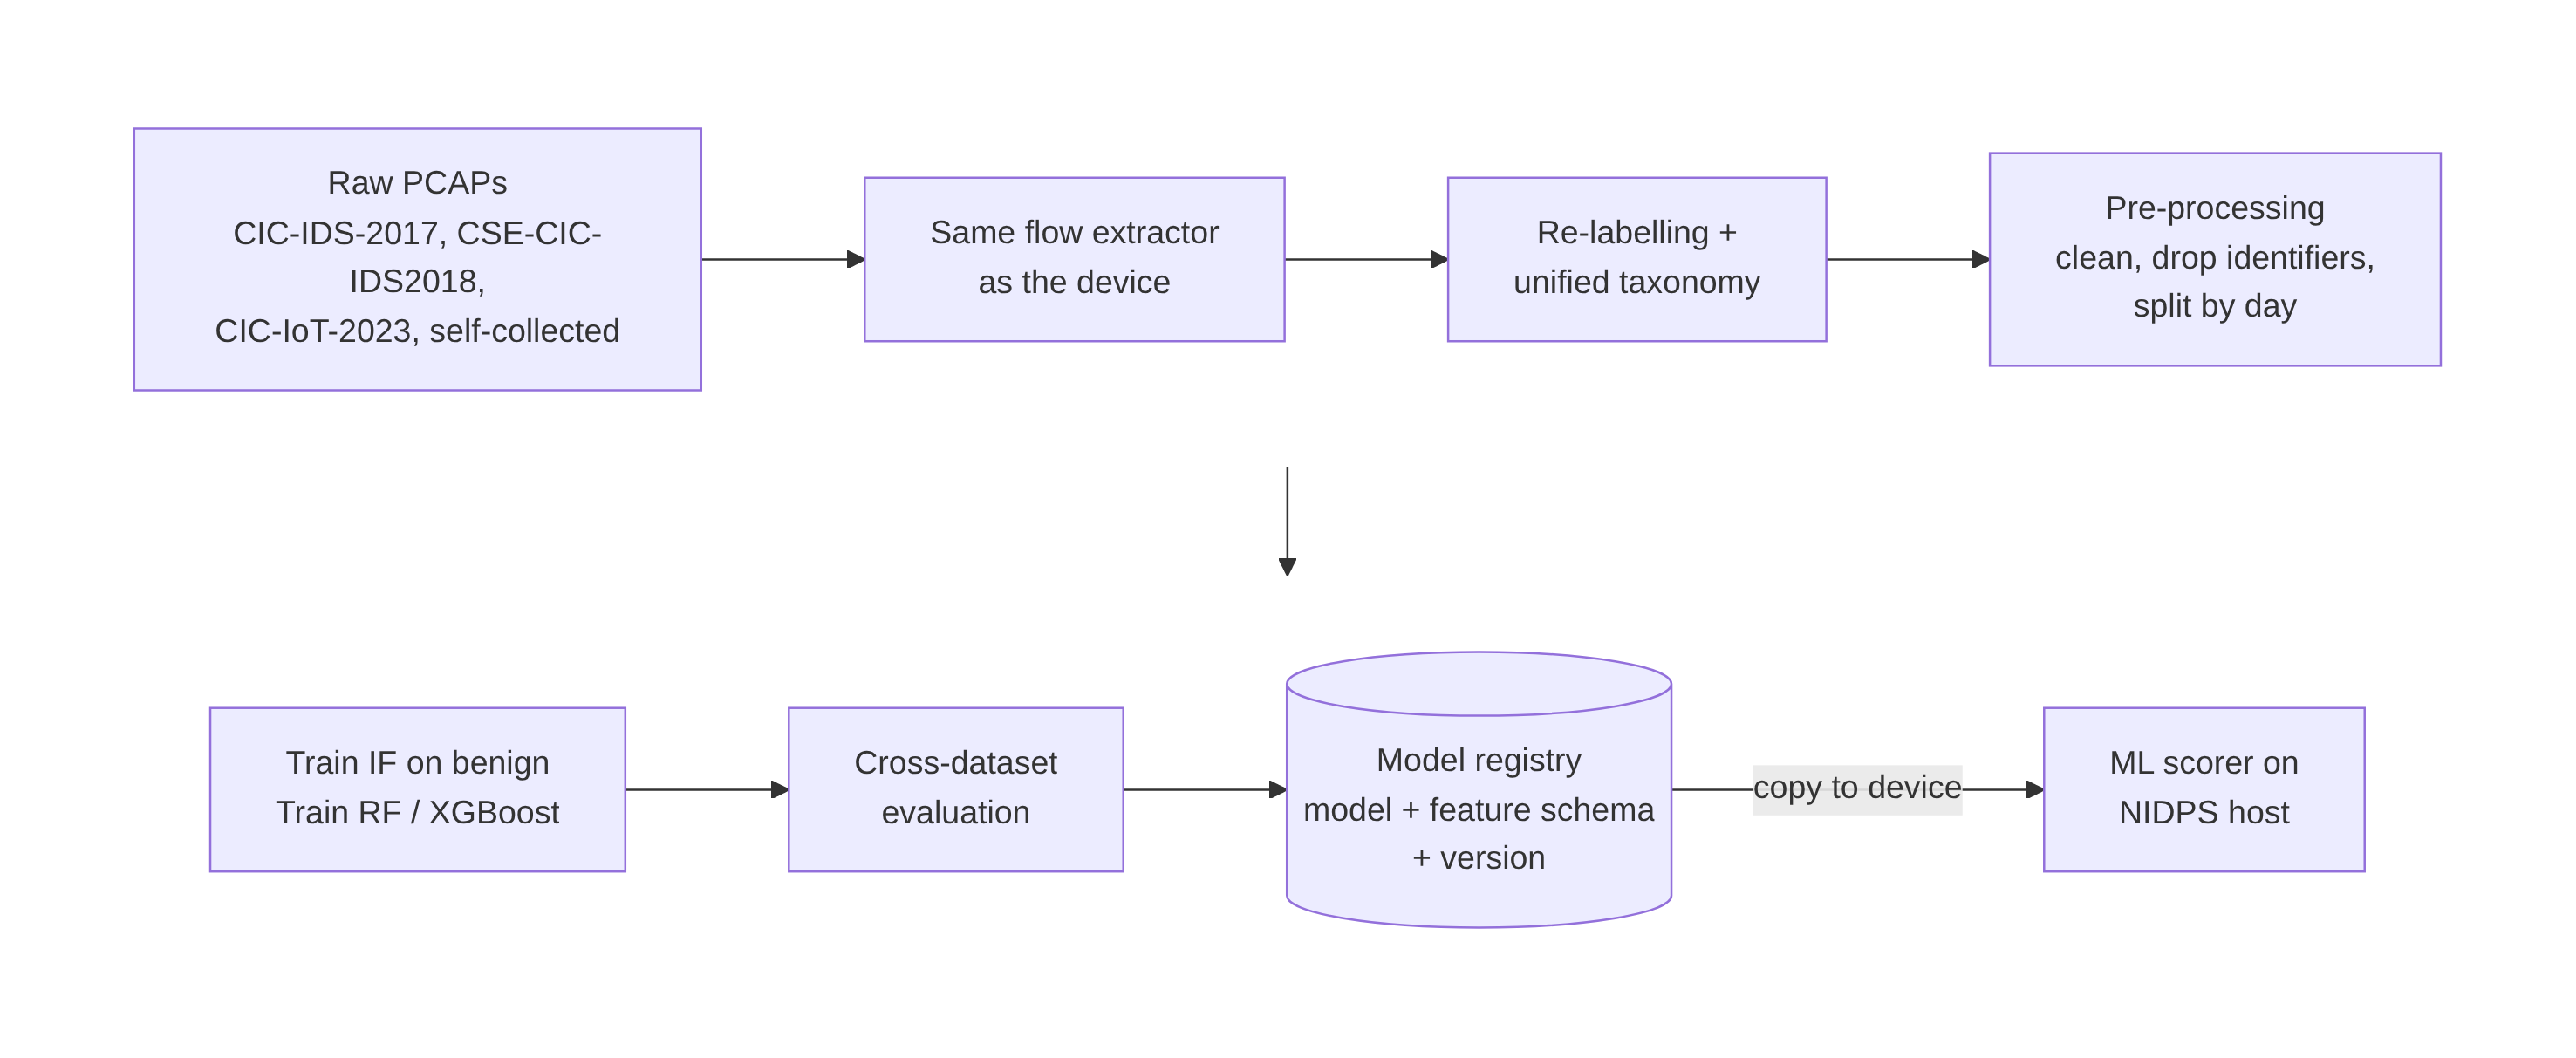
\includegraphics[width=0.9\textwidth]{Figures/nidps_fig6_3.png}
    \caption{Offline training pipeline and model hand-over to the device.}
    \label{fig:training}
\end{figure}

\noindent Training runs on a workstation, not on the NIDPS host, because it needs far more memory than inference. The only hand-over to the device is a model package containing the model file, its feature schema and a version manifest.

\section{Architectural Strategies}\label{sec:6.4}
\label{sec:archstrategies}
\noindent Each strategy below records the decision, the reasoning behind it and the alternatives that were rejected.

\subsection{Layered Defence with a Short Fast Path}\label{sec:6.4.1}
\noindent \textbf{Decision:} detection is split into a packet-level layer inside the forwarding path (Suricata) and flow-level layers outside it (ML), joined by a fusion step.

\noindent \textbf{Reasoning:} per-packet ML inference on every forwarded packet would exceed the CPU budget and add latency to every connection, violating the first goal of Section~\ref{sec:goals}. Flow-level ML outside the path costs nothing in forwarding latency, and Suricata covers the attacks that must be stopped at the first packet.

\noindent \textbf{Alternatives rejected:} ML-only inline detection (too slow, and no immediate protection against known attacks); Suricata-only detection (misses zero-day and behavioural attacks, the gap identified in Chapter~1).

\subsection{Metadata-Only Analysis of Encrypted Traffic}\label{sec:6.4.2}
\noindent \textbf{Decision:} encrypted traffic is analysed only through JA3/JA3S fingerprints and flow statistics.

\noindent \textbf{Reasoning:} TLS interception would require a trusted root certificate on every client, fails against certificate pinning, breaks some IoT devices outright and would multiply CPU load. It would also expose all household traffic in plain text on one device, which is a serious privacy risk.

\noindent \textbf{Alternatives rejected:} full TLS interception (above); ignoring encrypted traffic (most C2 now uses TLS). \textbf{Known limitation:} browsers now randomise TLS extension order, which makes JA3 less stable for browser traffic. Because fingerprinting is isolated in the flow extractor, it can be switched to JA4, which sorts extensions before hashing, without changing other components.

\subsection{Offline Training, Online Inference}\label{sec:6.4.3}
\noindent \textbf{Decision:} models are trained on a workstation and deployed as read-only, versioned packages. The device only performs inference and threshold calibration.

\noindent \textbf{Reasoning:} training on hundreds of millions of flows needs far more memory than the device has. Online retraining on the device would also let an attacker gradually teach the model that malicious traffic is normal (model poisoning). Recalibrating only the threshold (Section~\ref{sec:calibration}) adapts to the local network with bounded risk.

\noindent \textbf{Alternatives rejected:} continuous online learning (poisoning risk, hardware cost); a fixed global threshold (false positives on real home traffic).

\subsection{Local Services Connected by an Event Bus}\label{sec:6.4.4}
\noindent \textbf{Decision:} each component runs as its own systemd service, and components exchange messages through a local publish/subscribe bus. Redis Streams is the proposed implementation.

\noindent \textbf{Reasoning:} service isolation means a crash in one component does not take down the others, and systemd can restart each independently, which is a precondition for the failure modes. The bus decouples producers from consumers. Redis Streams is lightweight, keeps a bounded backlog that a restarted consumer can resume from, and supports consumer groups so the dashboard and the decision engine read the same events independently.

\noindent \textbf{Alternatives rejected:} direct function calls in one process (no fault isolation); Apache Kafka (far too heavy for the hardware); plain Unix sockets between each pair of components (simple, but every new consumer needs new wiring, and messages are lost while a consumer restarts). ZeroMQ was a close alternative and remains a fallback if Redis proves too heavy.

\subsection{Kernel-Enforced Blocking and Failure Semantics}\label{sec:6.4.5}
\noindent \textbf{Decision:} both blocking (ipset with timeouts) and the failure mode (NFQUEUE bypass or not) are enforced by the kernel, not by user-space software.

\noindent \textbf{Reasoning:} user-space components can crash; the kernel keeps running. Timed ipset entries expire even if the enforcer dies, so a crash never leaves hosts blocked forever, and the queue-bypass flag applies the chosen mode even if the watchdog is down.

\noindent \textbf{Alternatives rejected:} iptables rules added and deleted one per blocked host (slow with many entries and leaves stale rules after a crash); a user-space proxy that drops traffic (adds latency and is itself a crash risk).

\subsection{Choice of Languages and Products}\label{sec:6.4.6}
\noindent Table~\ref{tab:products} summarises the main product and language choices.

\begin{table}[H]
\centering
\caption{Product and language choices.}
\label{tab:products}
\begin{tabular}{|>{\raggedright\arraybackslash}p{0.13\linewidth}|>{\raggedright\arraybackslash}p{0.18\linewidth}|>{\raggedright\arraybackslash}p{0.3\linewidth}|>{\raggedright\arraybackslash}p{0.27\linewidth}|}
\hline
\textbf{Need} & \textbf{Choice} & \textbf{Main reason} & \textbf{Alternative considered} \\
\hline
Signature IPS & Suricata & Multi-threaded, native NFQUEUE IPS mode, EVE JSON output, TLS/JA3 support, maintained ET Open rules & Snort 3 (similar capability; Suricata chosen for its JSON output and threading) \\
\hline
Services and ML & Python 3 & scikit-learn and XGBoost available natively; fast development & C++ (faster, but much slower to develop; reconsidered only if profiling shows Python is the bottleneck) \\
\hline
Models & scikit-learn Isolation Forest and Random Forest, XGBoost & Small, fast tree models suited to tabular flow data & Deep autoencoders and LSTMs (higher compute cost, no clear gain on flow features) \\
\hline
Event store & SQLite & Zero administration, single file, enough for one device & PostgreSQL (needs a server process) \\
\hline
Dashboard & Python web API with WebSocket push and a lightweight web front end & Live updates with little code; reuses the Python stack & Grafana (heavy and less suited to showing verdict evidence and controls) \\
\hline
Firewall & iptables + ipset & Stated in the proposal; well documented; ipset handles large blocklists efficiently & nftables sets (modern equivalent; migration path kept open) \\
\hline
\end{tabular}
\end{table}

\subsection{Error Detection and Recovery}\label{sec:6.4.7}
\noindent Errors are handled at three levels.
\begin{enumerate}
    \item \textbf{Record level:} malformed flow records or alerts are rejected by the feature validator and counted, never passed to models.
    \item \textbf{Component level:} heartbeats and systemd supervision detect crashes and hangs and restart the component (Section~\ref{sec:failure}).
    \item \textbf{System level:} the kernel-enforced failure mode decides what happens to traffic while a component is down. All three levels log to the event store, so the dashboard can show when the system was not fully protected.
\end{enumerate}

\subsection{Data Storage, Persistence and Retention}\label{sec:6.4.8}
\label{sec:storage}
\noindent Only derived data is stored: alerts, verdicts, block records, host risk history, calibration state and configuration. Raw packets and payloads are never written to disk in normal operation. Flow records are kept for a short rolling window (for example, 7 days) for calibration and investigation, then deleted. This protects household privacy and keeps disk use bounded on a small device.

\subsection{Future Extension}\label{sec:6.4.9}
\noindent The architecture is designed so that the likely extensions require adding a component rather than changing existing ones: a new detector publishes to the bus; a new response (for example, notifying the owner's phone) subscribes to verdicts; a newer model or JA4 support is deployed as a new model package or extractor version.

\section{Domain Model/Class Diagram}\label{sec:6.5}
\label{sec:classdiagram}
\noindent Figure~\ref{fig:classdiagram} shows the main classes of the runtime system. The central entity is the Flow, which carries its features and optional TLS fingerprint through the pipeline. All detectors implement a common Detector interface and produce Evidence; the DecisionEngine turns Evidence into a Verdict, and the Enforcer turns BLOCK verdicts into BlockEntry records.

\begin{figure}[!htbp]
    \centering
    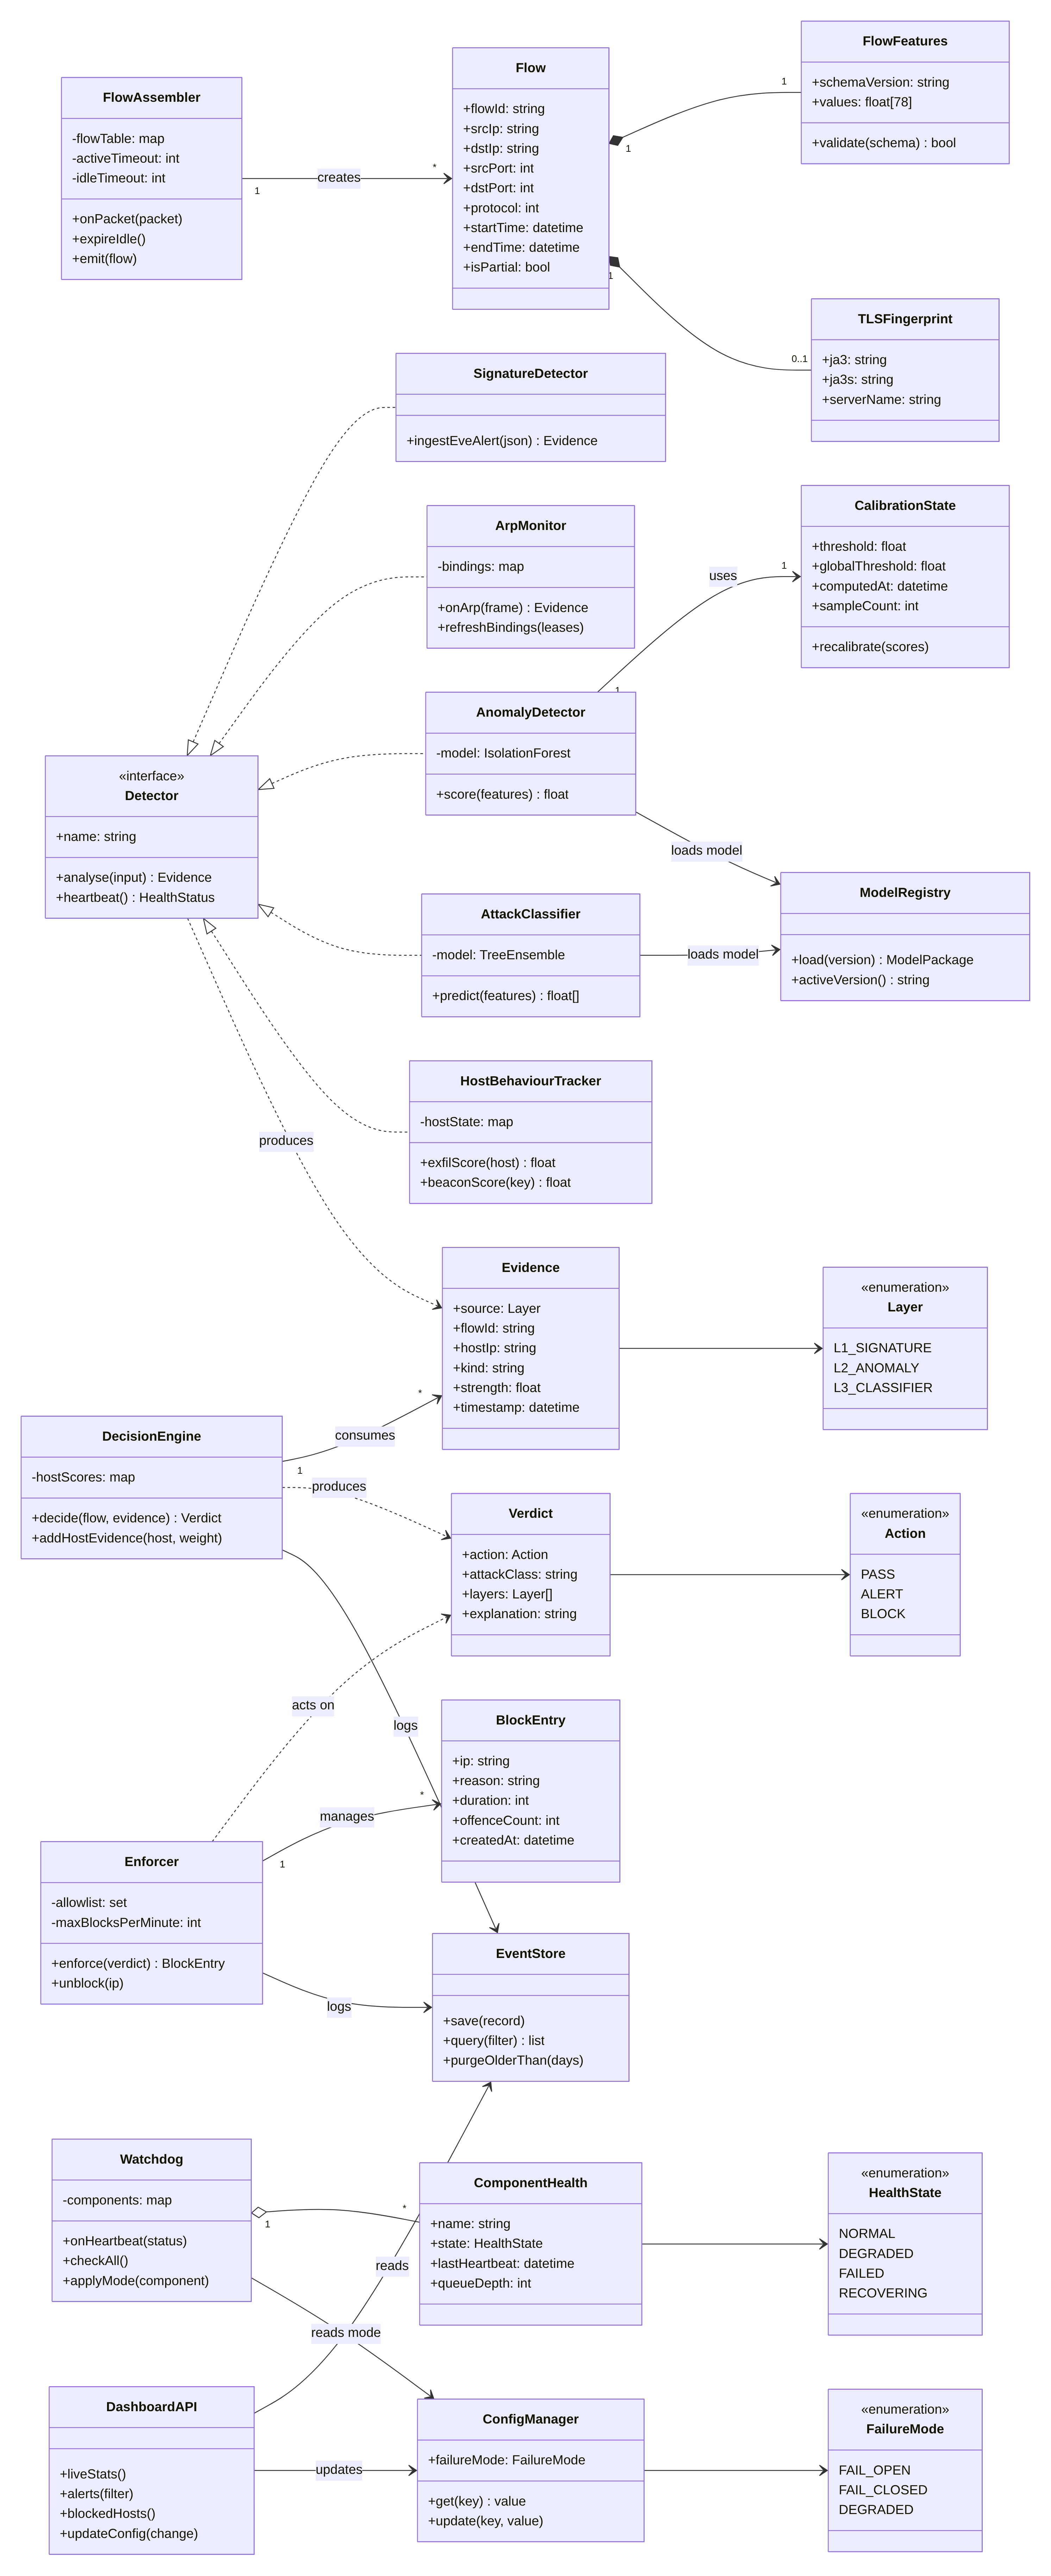
\includegraphics[height=0.85\textheight,keepaspectratio]{Figures/nidps_fig6_4.png}
    \caption{Class diagram of the NIDPS runtime.}
    \label{fig:classdiagram}
\end{figure}

\noindent The Detector interface is the main extension point: a new detection technique is added by implementing it and publishing its Evidence, without changes to the DecisionEngine. The Enforcer is the only class that changes firewall state, which keeps that responsibility in one small, auditable place.
\section{Policies and Tactics}\label{sec:6.6}
\label{sec:policies}
\noindent The following policies affect implementation details rather than the overall structure of the system.

\subsection{Rule and Threshold Management}\label{sec:6.6.1}
\noindent The ET Open ruleset is updated daily by a scheduled job, tested for syntax with Suricata's test mode, and loaded with a live rule reload so inspection never stops. If the test fails, the previous ruleset stays active. Custom rules live in a separate file under version control, so updates to ET rules never overwrite them. All numeric thresholds (rule thresholds, flow timeouts $T_a$ and $T_i$, $\tau$, $\theta$ values, $\Theta$, block durations) are read from one configuration file with documented defaults.

\subsection{Model Packaging and Versioning}\label{sec:6.6.2}
\label{sec:modelpackaging}
\noindent Each model package holds the model file, the ordered feature list with the extractor version, the class list and the training date and metrics. At load time the ML scorer refuses any package whose feature list does not match the running extractor. XGBoost models are stored in its native JSON format rather than as Python pickles, since loading a pickle can execute arbitrary code. scikit-learn models use joblib files, loaded only from the registry directory, which is writable only by the deployment user. The previous package is kept so a bad model can be rolled back with one command.

\subsection{Engineering Trade-offs}\label{sec:6.6.3}
\begin{itemize}
    \item \textbf{Detection speed vs.\ accuracy:} ML verdicts are per flow, not per packet (Section~\ref{sec:mltiming}), accepting a short delay for ML-detected attacks in exchange for zero added forwarding latency.
    \item \textbf{False positives vs.\ missed attacks:} the calibration percentile $p$ and the block thresholds are the explicit controls. Defaults lean towards fewer false positives, because wrong blocks on a home network cost the owner's trust quickly.
    \item \textbf{Availability vs.\ security:} chosen per deployment through the failure mode, with fail-open as the default for homes.
\end{itemize}

\subsection{Coding Guidelines and Conventions}\label{sec:6.6.4}
\noindent Python code follows PEP~8, uses type hints throughout and is checked with a linter and a type checker in continuous integration. Each service is a separate package with a single entry point. Messages on the event bus use a versioned JSON schema, so producers and consumers can be upgraded independently. Logs are structured JSON with a timestamp, component name and flow or host identifier, so events can be traced across services.

\subsection{Requirements Traceability}\label{sec:6.6.5}
\noindent Every goal from Chapter~\ref{chap:2} is mapped to the components that implement it and the tests that verify it, in a traceability matrix kept in the repository and updated at every sprint review (Table~\ref{tab:traceability}).

\begin{table}[H]
\centering
\caption{Requirements traceability matrix.}
\label{tab:traceability}
{\small
\begin{tabular}{|>{\raggedright\arraybackslash}p{0.3\linewidth}|>{\raggedright\arraybackslash}p{0.3\linewidth}|>{\raggedright\arraybackslash}p{0.3\linewidth}|}
\hline
\textbf{Proposal objective} & \textbf{Implemented by} & \textbf{Verified by} \\
\hline
Transparent inline NIDPS between clients and ISP gateway & Data plane (Section~\ref{sec:subsysarch}) & Connectivity and latency tests (Table~\ref{tab:sysperf}) \\
\hline
Suricata with ET ruleset for known attacks & SignatureDetector, custom rules (Section~\ref{sec:layer1}) & Live attack replay: SSH brute force, port scan, DNS spoofing \\
\hline
ML pipeline for anomaly detection and classification & AnomalyDetector, AttackClassifier, HostBehaviourTracker (Sections~\ref{sec:layer2}--\ref{sec:layer3}) & Detection metrics and live replay: C2 beaconing, exfiltration, DDoS, lateral movement \\
\hline
Cross-evaluation on three public datasets & Offline training pipeline (Figure~\ref{fig:training}) & Cross-dataset matrix (Table~\ref{tab:crossmatrix}) \\
\hline
Automatic blocking via iptables & Enforcer (Section~\ref{sec:prevention}) & Time-to-block measurement; allowlist and rate-limit tests \\
\hline
Watchdog and configurable failure handling & Watchdog, systemd units (Section~\ref{sec:failure}) & Fault-injection tests in each failure mode \\
\hline
Web dashboard & DashboardAPI (Section~\ref{sec:subsysarch}) & Functional UI tests; usability check with non-expert users \\
\hline
\end{tabular}
}
\end{table}

\subsection{Testing Plan}\label{sec:6.6.6}
\begin{enumerate}
    \item \textbf{Unit tests} for each algorithm: flow assembly on crafted PCAPs, JA3 computation against published reference hashes, threshold calibration, fusion rules and the enforcer's allowlist, rate limit and back-off.
    \item \textbf{Integration tests} that replay labelled PCAPs through the full pipeline on a test host and compare verdicts with labels.
    \item \textbf{Live attack tests} on the isolated lab network, executing each in-scope attack from the attacker machine against our own test devices.
    \item \textbf{Performance tests} for latency, throughput and resource use (Table~\ref{tab:sysperf}).
    \item \textbf{Fault-injection tests:} each service is killed or frozen under load in each failure mode, and recovery time and traffic impact are recorded.
    \item \textbf{Soak test:} the system runs for at least one week on a real home network in alert-only mode to measure false positives before blocking is enabled.
\end{enumerate}

\subsection{Hierarchical Organisation of the Source Code}\label{sec:6.6.7}
\noindent The source code is organised as follows:
{\footnotesize
\begin{verbatim}
nidps/
  dataplane/      hostapd, dnsmasq and netfilter configuration + setup scripts
  suricata/       suricata.yaml, custom.rules, rule-update job
  services/
    arpmon/       ARP consistency monitor
    flowextract/  flow assembler, feature computation, JA3/JA3S
    mlscorer/     feature validator, models, host behaviour tracker, calibration
    decision/     decision engine and host scores
    enforcer/     ipset management, allowlist, back-off
    watchdog/     heartbeat monitoring, state machine, failure modes
    dashboard/    web API and front end
  common/         bus client, message schemas, config loader, logging
  training/       dataset builder, labelling, training and evaluation scripts
  models/         model registry (versioned packages)
  deploy/         systemd unit files, install and upgrade scripts
  tests/          unit, integration, fault-injection tests and test PCAPs
  docs/           traceability matrix, design notes
\end{verbatim}
}

\subsection{Build and Deployment}\label{sec:6.6.8}
\noindent The system is installed on a fresh Debian-based image by one installation script that installs system packages (Suricata, hostapd, dnsmasq, ipset, Redis), creates a Python virtual environment with pinned dependency versions, copies the configuration and the active model package, and enables the systemd units in dependency order: data plane first, then Suricata, then the remaining services. Upgrades replace one service at a time and restart only that service. Because every service is supervised and the failure mode is kernel-enforced, an upgrade never leaves the network without a defined behaviour.

\subsection{Maintenance}\label{sec:6.6.9}
\noindent Routine maintenance is automated: daily rule updates, weekly threshold recalibration (Algorithm~\ref{alg:calibration}), and log and flow-record purging beyond the retention window. Models are retrained offline when new datasets or significant new attack classes become available, or when the dashboard shows a rising alert rate that calibration does not explain. Component health history on the dashboard tells the owner when the system has been running in a degraded or failed state.

\section{Conclusion}\label{sec:6.7}
\label{sec:ch6conclusion}
\noindent This chapter translated the methodology of Chapter~\ref{chap:approach} into a concrete design. The NIDPS is a single Linux host organised as five runtime subsystems (data plane, detection, decision and response, management and reporting, and reliability) plus an offline training pipeline. The main architectural decisions keep the forwarding path short, analyse encrypted traffic only through metadata, train offline while calibrating thresholds online, isolate components as supervised services connected by an event bus, and let the kernel enforce both blocking and failure behaviour. The class diagram defines a common Detector interface that makes new detectors easy to add, while confining firewall changes to a single Enforcer. The policies on rule and model management, testing, traceability and deployment complete the design and connect each proposal objective to the component that delivers it and the test that verifies it.


\bibliographystyle{ieeetr}
\bibliography{fypbib}

\end{document}
